%%%%%%%%%%%%%%%%%%%%%%%%%%%%%%%%%%%%%%%%%%%%%%%%%%%%%%%%%%%%%%%%%%%%%%%%%
%  Zawartość: Główny plik szablonu pracy dyplomowej (magisterskiej/inżynierskiej).
%  Opracował: Tomasz Kubik <tomasz.kubik@pwr.edu.pl>
%  Data: kwiecień 2016
%  Wersja: 0.2
%%%%%%%%%%%%%%%%%%%%%%%%%%%%%%%%%%%%%%%%%%%%%%%%%%%%%%%%%%%%%%%%%%%%%%%%%

\documentclass[a4paper,onecolumn,oneside,12pt,extrafontsizes]{memoir}
% W celu przygotowania wydruku do archiwum należy przesłonić komendę powyższą
% dwoma poniższymi komendami:
%\documentclass[a4paper,onecolumn,twoside,10pt]{memoir} 
%\renewcommand{\normalsize}{\fontsize{8pt}{10pt}\selectfont}

%\usepackage[cp1250]{inputenc} % jeśli kodowanie edytowanych plików to cp1250 
\usepackage[utf8]{inputenc} % jeśli kodowanie edytowanych plików to UTF8
\usepackage[T1]{fontenc}
\usepackage[polish]{babel}
%\DisemulatePackage{setspace}
\usepackage{setspace}
\usepackage{tabularx}
\usepackage[table,xcdraw]{xcolor}
\usepackage[nodayofweek,level]{datetime}
\usepackage{placeins}
\usepackage{csquotes}
\usepackage{color,calc}
%\usepackage{soul} % pakiet z komendami do podkreślania tekstu

\usepackage{ebgaramond} % pakiet z czcionkami garamond, potrzebny tylko do strony tytułowej, musi wystąpić przed pakietem tgtermes

%% Aby uzyskać polskie literki w pdfie (a nie zlepki) korzystamy z pakietu czcionek tgterms. 
%% W pakiecie tym są zdefiniowane klony czcionek Times o kształtach: normalny, pogrubiony, italic, italic pogrubiony.
%% W pakiecie tym brakuje czcionki o kształcie: slanted (podobny do italic). 
%% Jeśli w dokumencie gdzieś zostanie zastosowana czcionka slanted (np. po użyciu komendy \textsl{}), to
%% latex dokona podstawienia na czcionkę standardową i zgłosi to w ostrzeżeniu (warningu).
%% Ponadto tgtermes to czcionka do tekstu. Wszelkie matematyczne wzory będą sformatowane domyślną czcionką do wzorów.
%% Jeśli wzory mają być sformatowane z wykorzystaniem innych czcionek, trzeba to jawnie zadeklarować.

%% Po zainstalowaniu pakietu tgtermes może będzie trzeba zauktualizować informacje 
%% o dostępnych fontach oraz mapy. Można to zrobić z konsoli (jako administrator)
%% initexmf --admin --update-fndb
%% initexmf --admin --mkmaps

\hyphenation{SPORTident}
\usepackage{tgtermes}   
\renewcommand*\ttdefault{txtt}

% We wcześniejszej wersji szablonu korzystano z innych czcionek. Dla celów historycznych pozostawiono je w komentarzu
%\usepackage{mathptmx} % pakiet będący następcą pakietów times and mathptm, niestety polskie literki są zlepkami
%\usepackage{newtxtext,newtxmath} % pakiety dostarczające Times dla tekstów i wzorów matematycznych,  
%                                  rozwiązuje problemy występujące w mathptmx, ale wymaga zainstalowania
%                                  dodatkowych pakietów oraz uruchomienia updmap (konsola administratora)
%                                  niestety polskie literki są zlepkami
%\usepackage{newtxmath,tgtermes} % można też połączyć czcionki do tekstu i czcionki do wzorów

\usepackage{listings}
\lstloadlanguages{% Check Dokumentation for further languages ...
C,
C++,
csh,
Java
}

\definecolor{red}{rgb}{0.6,0,0} % for strings
\definecolor{blue}{rgb}{0,0,0.6}
\definecolor{green}{rgb}{0,0.8,0}
\definecolor{cyan}{rgb}{0.0,0.6,0.6}

\lstset{
language=csh,
basicstyle=\footnotesize\ttfamily, 
numbers=left, 
numberstyle=\tiny, 
numbersep=5pt, 
tabsize=2, 
extendedchars=true, 
escapeinside={\%*}{*)},
breaklines=true, 
frame=b,
stringstyle=\color{blue}\ttfamily, 
showspaces=false, 
showtabs=true, 
xleftmargin=17pt,
framexleftmargin=17pt,
framexrightmargin=5pt,
framexbottommargin=4pt,
commentstyle=\color{green},
morecomment=[l]{//}, %use comment-line-style!
morecomment=[s]{/*}{*/}, %for multiline comments
showstringspaces=false, 
morekeywords={  abstract, event, new, struct,
                as, explicit, null, switch,
                base, extern, object, this,
                bool, false, operator, throw,
                break, finally, out, true,
                byte, fixed, override, try,
                case, float, params, typeof,
                catch, for, private, uint,
                char, foreach, protected, ulong,
                checked, goto, public, unchecked,
                class, if, readonly, unsafe,
                const, implicit, ref, ushort,
                continue, in, return, using,
                decimal, int, sbyte, virtual,
                default, interface, sealed, volatile,
                delegate, internal, short, void,
                do, is, sizeof, while,
                double, lock, stackalloc,
                else, long, static,
                enum, namespace, string},
keywordstyle=\color{cyan},
identifierstyle=\color{red},
}

% Choć możliwe jest zastosowanie różnych pakietów formatujących tabele, zaleca się tego nie robić.
%\usepackage{longtable}
%\usepackage{ltxtable}
%\usepackage{tabulary}

%%%%%%%%%%%%%%%%%%%%%%%%%%%%%%%%%%%%%%%%%%%%%%%%%%%
%% Ustawienia odpowiedzialne za sposób łamania dokumentu
%% i ułożenie elementów pływających
%%%%%%%%%%%%%%%%%%%%%%%%%%%%%%%%%%%%%%%%%%%%%%%%%%%
%\hyphenpenalty=10000		% nie dziel wyrazów zbyt często
\clubpenalty=10000      %kara za sierotki
\widowpenalty=10000  % nie pozostawiaj wdów
\brokenpenalty=10000		% nie dziel wyrazów między stronami
\exhyphenpenalty=999999		% nie dziel słów z myślnikiem
\righthyphenmin=3			% dziel minimum 3 litery

%\tolerance=4500
%\pretolerance=250
%\hfuzz=1.5pt
%\hbadness=1450

\renewcommand{\topfraction}{0.95}
\renewcommand{\bottomfraction}{0.95}
\renewcommand{\textfraction}{0.05}
\renewcommand{\floatpagefraction}{0.35}

%%%%%%%%%%%%%%%%%%%%%%%%%%%%%%%%%%%%%%%%%%%%%%%%%%%
%%  Ustawienia rozmiarów: tekstu, nagłówka i stopki, marginesów
%%  dla dokumentów klasy memoir 
%%%%%%%%%%%%%%%%%%%%%%%%%%%%%%%%%%%%%%%%%%%%%%%%%%%
\setlength{\headsep}{10pt} 
\setlength{\headheight}{13.6pt} % wartość baselineskip dla czcionki 11pt tj. \small wynosi 13.6pt
\setlength{\footskip}{\headsep+\headheight}
\setlength{\uppermargin}{\headheight+\headsep+1cm}
\setlength{\textheight}{\paperheight-\uppermargin-\footskip-1.5cm}
\setlength{\textwidth}{\paperwidth-5cm}
\setlength{\spinemargin}{2.5cm}
\setlength{\foremargin}{2.5cm}
\setlength{\marginparsep}{2mm}
\setlength{\marginparwidth}{2.3mm}
%\settrimmedsize{297mm}{210mm}{*}
%\settrims{0mm}{0mm}	
\checkandfixthelayout[fixed] % konieczne, aby się dobrze wszystko poustawiało
%%%%%%%%%%%%%%%%%%%%%%%%%%%%%%%%%%%%%%%%%%%%%%%%
%%  Ustawienia odległości linii, wcięć, odstępów
%%%%%%%%%%%%%%%%%%%%%%%%%%%%%%%%%%%%%%%%%%%%%%%%
\linespread{1}
%\linespread{1.241}
\setlength{\parindent}{14.5pt}
%\setbeforesecskip{10pt plus 0.5ex}%{-3.5ex \@plus -1ex \@minus -.2ex}
%\setaftersecskip{10pt plus 0.5ex}%\onelineskip}
%\setbeforesubsecskip{8pt plus 0.5ex}%{-3.5ex \@plus -1ex \@minus -.2ex}
%\setaftersubsecskip{8pt plus 0.5ex}%\onelineskip}
%\setlength\floatsep{6pt plus 2pt minus 2pt} 
%\setlength\intextsep{12pt plus 2pt minus 2pt} 
%\setlength\textfloatsep{12pt plus 2pt minus 2pt} 

%%%%%%%%%%%%%%%%%%%%%%%%%%%%%%%%%%%%%%%%%%%%%%%%%%%
%%  Pakiety i komendy zastosowane tylko do zamieszczenia informacji o użytych komendach i fontach
%%  Normalnie nie są potrzebne, można je zamarkować podczas redakcji pracy
%%%%%%%%%%%%%%%%%%%%%%%%%%%%%%%%%%%%%%%%%%%%%%%%%%%
\usepackage{memlays}     % extra layout diagrams, zastosowane w szblonie do 'debuggowania', używa pakietu layouts
%\usepackage{layouts}
\usepackage{printlen} % pakiet do wyświetlania wartości zdefiniowanych długości, stosowany do 'debuggowania'
\uselengthunit{pt}
\makeatletter
\newcommand{\showFontSize}{\f@size pt} % makro wypisujące wielkość bieżącej czcionki
\makeatother
% do pokazania ramek można byłoby użyć:
%\usepackage{showframe} 


%%%%%%%%%%%%%%%%%%%%%%%%%%%%%%%%%%%%%%%%%%%%%%%%%%%
%%  Formatowanie list wyliczeniowych, wypunktowań i własnych otoczeń
%%%%%%%%%%%%%%%%%%%%%%%%%%%%%%%%%%%%%%%%%%%%%%%%%%%

% Domyślnie wypunktowania mają zadeklatorowane znaki, które nie występują w tgtermes
% Aby latex nie podstawiał w ich miejsca znaków z czcionki standardowej można zrobić podstawienie:
%    \DeclareTextCommandDefault{\textbullet}{\ensuremath{\bullet}}
%    \DeclareTextCommandDefault{\textasteriskcentered}{\ensuremath{\ast}}
%    \DeclareTextCommandDefault{\textperiodcentered}{\ensuremath{\cdot}}
% Jednak jeszcze lepszym pomysłem jest zdefiniowanie otoczeń z wykorzystaniem enumitem
\usepackage{enumitem} % pakiet pozwalający zarządzać formatowaniem list wyliczeniowych
\setlist{noitemsep,topsep=4pt,parsep=0pt,partopsep=4pt,leftmargin=*} % zadeklarowane parametry pozwalają uzyskać 'zwartą' postać wypunktowania bądź wyliczenia
\setenumerate{labelindent=0pt,itemindent=0pt,leftmargin=!,label=\arabic*.} % można zmienić \arabic na \alph, jeśli wyliczenia mają być z literkami
\setlistdepth{4} % definiujemy głębokość zagnieżdżenia list wyliczeniowych do 4 poziomów
\setlist[itemize,1]{label=$\bullet$}  % definiujemy, jaki symbol ma być użyty w wyliczeniu na danym poziomie
\setlist[itemize,2]{label=\normalfont\bfseries\textendash}
\setlist[itemize,3]{label=$\ast$}
\setlist[itemize,4]{label=$\cdot$}
\renewlist{itemize}{itemize}{4}

%%%http://tex.stackexchange.com/questions/29322/how-to-make-enumerate-items-align-at-left-margin
%\renewenvironment{enumerate}
%{
%\begin{list}{\arabic{enumi}.}
%{
%\usecounter{enumi}
%%\setlength{\itemindent}{0pt}
%%\setlength{\leftmargin}{1.8em}%{2zw} % 
%%\setlength{\rightmargin}{0zw} %
%%\setlength{\labelsep}{1zw} %
%%\setlength{\labelwidth}{3zw} % 
%\setlength{\topsep}{6pt}%
%\setlength{\partopsep}{0pt}%
%\setlength{\parskip}{0pt}%
%\setlength{\parsep}{0em} % 
%\setlength{\itemsep}{0em} % 
%%\setlength{\listparindent}{1zw} % 
%}
%}{
%\end{list}
%}

\makeatletter
\renewenvironment{quote}{
	\begin{list}{}
	{
	\setlength{\leftmargin}{1em}
	\setlength{\topsep}{0pt}%
	\setlength{\partopsep}{0pt}%
	\setlength{\parskip}{0pt}%
	\setlength{\parsep}{0pt}%
	\setlength{\itemsep}{0pt}
	}
	}{
	\end{list}}
\makeatother

%%%%%%%%%%%%%%%%%%%%%%%%%%%%%%%%%%%%%%%%%
%%  Pakiet do generowania indeksu (ważne, aby wstawić przed hyperref)
%%%%%%%%%%%%%%%%%%%%%%%%%%%%%%%%%%%%%%%%%
\DisemulatePackage{imakeidx}
\usepackage[makeindex,noautomatic]{imakeidx} % tutaj mówimy, żeby indeks nie generował się automatycznie, 

%\usepackage[noautomatic]{imakeidx} 
\makeindex

\makeatletter
%%%\renewenvironment{theindex}
							 %%%{\vskip 10pt\@makeschapterhead{\indexname}\vskip -3pt%
								%%%\@mkboth{\MakeUppercase\indexname}%
												%%%{\MakeUppercase\indexname}%
								%%%\vspace{-3.2mm}\parindent\z@%
								%%%\renewcommand\subitem{\par\hangindent 16\p@ \hspace*{0\p@}}%%
								%%%\phantomsection%
								%%%\begin{multicols}{2}
								%%%%\thispagestyle{plain}
								%%%\parindent\z@                
								%%%%\parskip\z@ \@plus .3\p@\relax
								%%%\let\item\@idxitem}
							 %%%{\end{multicols}\clearpage}
%%%
\makeatother


\usepackage{ifpdf}
%\newif\ifpdf \ifx\pdfoutput\undefined
%\pdffalse % we are not running PDFLaTeX
%\else
%\pdfoutput=1 % we are running PDFLaTeX
%\pdftrue \fi
\ifpdf
 \usepackage[pdftex,bookmarks,breaklinks,unicode]{hyperref}
 \usepackage[pdftex]{graphicx}
 \graphicspath{ {images/} }
 \DeclareGraphicsExtensions{.pdf,.jpg,.mps,.png}
\pdfcompresslevel=9
\pdfoutput=1
\makeatletter
\AtBeginDocument{
  \hypersetup{
	pdfinfo={
    Title = {\@title},
    Author = {\@author},
    Subject={},
    Keywords={},
  }}
}
\makeatother
\else
\usepackage{graphicx}
\DeclareGraphicsExtensions{.eps,.ps,.jpg,.mps,.png}
\fi
\sloppy

%\graphicspath{{rys01/}{rys02/}}


%%%%%%%%%%%%%%%%%%%%%%%%%%%%%%%%%%%%%%%%%
% Metadane dla pdfa


%\ifpdf
%\pdfinfo{
   %/Author (Nicola Talbot)
   %/Title  (Creating a PDF document using PDFLaTeX)
   %/CreationDate (D:20040502195600)
   %/ModDate (D:\pdfdate)
   %/Subject (PDFLaTeX)
   %/Keywords (PDF;LaTeX)
%}
%\fi

% Deklaracja głębokościu numeracji
\setcounter{secnumdepth}{2}
\setcounter{tocdepth}{2}
\setsecnumdepth{subsection} % activating subsubsec numbering in doc


% Kropki po numerach sekcji
\makeatletter
\def\@seccntformat#1{\csname the#1\endcsname.\quad}
\def\numberline#1{\hb@xt@\@tempdima{#1\if&#1&\else.\fi\hfil}}
\makeatother

\renewcommand{\chapternumberline}[1]{#1.\quad}
\renewcommand{\cftchapterdotsep}{\cftdotsep}

%\definecolor{niceblue}{rgb}{.168,.234,.671}

% Czcionka do podpisów tabel i rysunków
\captionnamefont{\small}
\captiontitlefont{\small}
% makro pozwalające zmienić sposób wypisywania rozdziału
%\def\printchaptertitle##1{\fonttitle \space \thechapter.\space ##1} 

%\usepackage{ltcaption}
% The ltcaption package supports \CaptionLabelFont & \CaptionTextFont introduced by the NTG document classes
%\renewcommand\CaptionLabelFont{\small}
%\renewcommand\CaptionTextFont{\small}

% Przedefiniowanie etykiet w podpisach tabel i rysunków
%\AtBeginDocument{% 
        \addto\captionspolish{% 
        \renewcommand{\tablename}{Tab.}% 
}%} 

%\AtBeginDocument{% 
%        \addto\captionspolish{% 
%        \renewcommand{\chaptername}{Rozdział}% 
%}} 

%\AtBeginDocument{% 
        \addto\captionspolish{% 
        \renewcommand{\figurename}{Rys.}% 
}%}


%\AtBeginDocument{% 
        \addto\captionspolish{% 
        \renewcommand{\bibname}{Literatura}% 
}%}

%\AtBeginDocument{% 
        \addto\captionspolish{% 
        \renewcommand{\listfigurename}{Spis rysunków}% 
}%}

%\AtBeginDocument{% 
        \addto\captionspolish{% 
        \renewcommand{\listtablename}{Spis tabel}% 
}%}

%\AtBeginDocument{% 
        \addto\captionspolish

%%%%%%%%%%%%%%%%%%%%%%%%%%%%%%%%%%%%%%%%%%%%%%%%%%%%%%%%%%%%%%%%%%                  
%% Definicje stopek i nagłówków
%%%%%%%%%%%%%%%%%%%%%%%%%%%%%%%%%%%%%%%%%%%%%%%%%%%%%%%%%%%%%%%%%%                  
\addtopsmarks{headings}{%
\nouppercaseheads % added at the beginning
}{%
\createmark{chapter}{both}{shownumber}{}{. \space}
%\createmark{chapter}{left}{shownumber}{}{. \space}
\createmark{section}{right}{shownumber}{}{. \space}
}%use the new settings

\makeatletter
\copypagestyle{outer}{headings}
\makeoddhead{outer}{}{}{\small\itshape\rightmark}
\makeevenhead{outer}{\small\itshape\leftmark}{}{}
\makeoddfoot{outer}{\small\@author:~\@titleShort}{}{\small\thepage}
\makeevenfoot{outer}{\small\thepage}{}{\small\@author:~\@title}
\makeheadrule{outer}{\linewidth}{\normalrulethickness}
\makefootrule{outer}{\linewidth}{\normalrulethickness}{2pt}
\makeatother

% fix plain
\copypagestyle{plain}{headings} % overwrite plain with outer
\makeoddhead{plain}{}{}{} % remove right header
\makeevenhead{plain}{}{}{} % remove left header
\makeevenfoot{plain}{}{}{}
\makeoddfoot{plain}{}{}{}

\copypagestyle{empty}{headings} % overwrite plain with outer
\makeoddhead{empty}{}{}{} % remove right header
\makeevenhead{empty}{}{}{} % remove left header
\makeevenfoot{empty}{}{}{}
\makeoddfoot{empty}{}{}{}


%%%%%%%%%%%%%%%%%%%%%%%%%%%%%%%%%%%%%%%
%% Definicja strony tytułowej 
%%%%%%%%%%%%%%%%%%%%%%%%%%%%%%%%%%%%%%%
\makeatletter
%Uczelnia
\newcommand\uczelnia[1]{\renewcommand\@uczelnia{#1}}
\newcommand\@uczelnia{}
%Wydział
\newcommand\wydzial[1]{\renewcommand\@wydzial{#1}}
\newcommand\@wydzial{}
%Kierunek
\newcommand\kierunek[1]{\renewcommand\@kierunek{#1}}
\newcommand\@kierunek{}
%Specjalność
\newcommand\specjalnosc[1]{\renewcommand\@specjalnosc{#1}}
\newcommand\@specjalnosc{}
%Tytuł po angielsku
\newcommand\titleEN[1]{\renewcommand\@titleEN{#1}}
\newcommand\@titleEN{}
%Tytuł krótki
\newcommand\titleShort[1]{\renewcommand\@titleShort{#1}}
\newcommand\@titleShort{}
%Promotor
\newcommand\promotor[1]{\renewcommand\@promotor{#1}}
\newcommand\@promotor{}

%\usepackage[absolute]{textpos} % zamarkowano, bo ostatecznie wykorzystano otoczenie picture

\def\maketitle{%
  \pagestyle{empty}%
%%\garamond 
	\fontfamily{\ebgaramond@family}\selectfont % na stronie tytułowej czcionka garamond
%%%%%%%%%%%%%%%%%%%%%%%%%%%%%%%%%%%%%	
%% Poniżej, w otoczniu picture, wstawiono tytuł i autora. 
%% Tytuł (z autorem) musi znaleźć się w obszarze 
%% odpowiadającym okienku 110mmx75mm, którego lewy górny róg 
%% jest w położeniu 77mm od lewej i 111mm od górnej  krawędzi strony 
%% (tak wynika z wycięcia na okładce). 
%% Poniższy kod musi być użyty dokładnie w miejscu gdzie jest.
%% Jeśli tytuł nie mieści się w okienku, to należy tak pozmieniać 
%% parametry użytych komend, aby ten przydługi tytuł jednak 
%% upakować go do okienka.
%%
%% Sama okładka (kolorowa strona z wycięciem, do pobrania z dydaktyki) 
%% powinna być przycięta o 3mm od każdej z krawędzi.
%% Te 3mm pewnie zostawiono na ewentualne spady czy też specjalną oprawę.
%%%%%%%%%%%%%%%%%%%%%%%%%%%%%%%%%%%%%	
\newlength{\tmpfboxrule}
\setlength{\tmpfboxrule}{\fboxrule}
\setlength{\fboxsep}{2mm}
\setlength{\fboxrule}{0mm} 
%\setlength{\fboxrule}{0.1mm} %% jeśli chcemy zobaczyć ramkę
\setlength{\unitlength}{1mm}
\begin{picture}(0,0)
\put(26,-124){\fbox{
\parbox[c][71mm][c]{104mm}{\centering%\lineskip=34pt 
\fontsize{16pt}{18pt}\selectfont \@title\\[5mm]
%\fontsize{16pt}{18pt}\selectfont \@titleEN\\[20mm]
\fontsize{16pt}{18pt}\selectfont AUTORZY:\\[2mm]
\fontsize{14pt}{16pt}\selectfont \@author}
}
}
\end{picture}
\setlength{\fboxrule}{\tmpfboxrule} 
%%%%%%%%%%%%%%%%%%%%%%%%%%%%%%%%%%%%%
%% Reszta strony z nazwą uczelni, wydziału, kierunkiem, specjalnością
%% promotorem, oceną pracy, miastem i rokiem
	{\centering%\vspace{-1cm}
		{\fontsize{22pt}{24pt}\selectfont \@uczelnia}\\[0.4cm]
		{\fontsize{22pt}{24pt}\selectfont \@wydzial}\\[0.5cm]
		  \hrule %\vspace*{0.7cm}
	}
{\flushleft\fontsize{14pt}{16pt}\selectfont%
\begin{tabular}{ll}
KIERUNEK: & \@kierunek\\
%SPECJALNOŚĆ: & \@specjalnosc\\
\end{tabular}\\[1.3cm]
}
{\centering
{\fontsize{24pt}{36pt}\selectfont PROJEKT}\\[0.5cm]
{\fontsize{24pt}{36pt}\selectfont Teoria i inżynieria ruchu teleinformatycznego}\\[2.5cm]
}
\vfill
%\begin{tabularx}{\linewidth}{p{6cm}l}
%		&{\fontsize{16pt}{18pt}\selectfont PROWADZĄCY PRACĘ:}\\[2mm] %UWAGA: tutaj jest miejsce na nazwisko promotora pracy
%		&{\fontsize{14pt}{16pt}\selectfont \@promotor}\\[10mm]
%		&{\fontsize{16pt}{18pt}\selectfont OCENA PRACY:}\\[20mm]
%	\end{tabularx}
\vspace{2cm}
\hrule\vspace*{0.3cm}
{\centering
{\fontsize{16pt}{18pt}\selectfont \@date}\\[0cm]
}
%\ungaramond
\normalfont
 \cleardoublepage
}
\makeatother
%%%%%%%%%%%%%%%%%%%%%%%%%%%%%%%%%%%%%%%%%

%\AtBeginDocument{\addtocontents{toc}{\protect\thispagestyle{empty}}}




%%%%%%%%%%%%%%%%%%%%%%%%%%%%%%%%%%%%%%%%%
%%  Metadane dokumentu 
%%%%%%%%%%%%%%%%%%%%%%%%%%%%%%%%%%%%%%%%%
\title{Analiza sieci systemów autonomicznych przy użyciu algorytmów grafowych}
%\titleShort{Szablon pracy dyplomowej ...}
\author{Bartosz Cieśla, Bartosz Janusz, Bartosz Kardas}
\uczelnia{POLITECHNIKA WROCŁAWSKA}
\wydzial{WYDZIAŁ INFORMATYKI I ZARZĄDZANIA}
\kierunek{INFORMATYKA}
\specjalnosc{INŻYNIERIA INTERNETOWA}
%\promotor{A}
\date{WROCŁAW, 2017}

% Ustawienie odstępu od góry w nienumerowanych rozdziałach oraz wykazach:
% Spis treści, Spis tabel, Spis rysunków, Indeks rzeczowy

%\newlength{\linespace}
%\setlength{\linespace}{-\beforechapskip-\topskip+\headheight+\topsep}
%\makechapterstyle{noNumbered}{%
%\renewcommand\chapterheadstart{\vspace*{\linespace}}
%}

%% powyższa komenda załatwia to, co robią komendy poniższe dla spisów
%\renewcommand*{\tocheadstart}{\vspace*{\linespace}}
%\renewcommand*{\lotheadstart}{\vspace*{\linespace}}
%\renewcommand*{\lofheadstart}{\vspace*{\linespace}}

%%%%%%%%%%%%%%%%%%%%%%%%%%%%%%%%%%%%%%%%%
%                  Początek dokumentu 
%%%%%%%%%%%%%%%%%%%%%%%%%%%%%%%%%%%%%%%%%
%\includeonly{skroty,rozdzial01} % jeśli chcemy kompilować tylko fragmenty, to można tu je wpisać

\begin{document}
% Tutaj można przełączyć odstęp między liniami
%\SingleSpacing
%\OnehalfSpacing
%\DoubleSpacing

%\settypeoutlayoutunit{cm} % do debugowania
%\typeoutstandardlayout    % wypisuje na stdout informacje o ustawieniach
\maketitle

\newpage
%\thispagestyle{empty}
%\mbox{}\vfill
%\noindent\begin{tabular}{@{}ll} Opracował: & Tomasz Kubik %<tomasz.kubik@pwr.edu.pl>\\
% Data: & maj 2016 
% \end{tabular}\\[15mm]
%\noindent\includegraphics[width=3cm]{by-nc-sa}\newline
%{\normalfont 
%Szablon jest udostępniany na licencji Creative Commons: \emph{Uznanie autorstwa -- Użycie niekomercyjne -- Na tych samych warunkach, 3.0 Polska}, Wrocław 2016. \\[2pt]
%Oznacza to, że wszystkie zawarte  nim treści można kopiować i  wykorzystywać do celów niekomercyjnych, a także tworzyć na ich podstawie utwory zależne pod warunkiem podania autora i~nazwy licencjodawcy oraz udzielania na utwory zależne takiej samej licencji. Tekst licencji jest dostępny pod adresem: \url{http://creativecommons.org/licenses/by-nc-sa/3.0/pl/}.}
%\newpage


\chapterstyle{noNumbered}
\pagestyle{outer}
\mbox{}\pdfbookmark[0]{Spis treści}{spisTresci.1}
\tableofcontents* 

\newpage
\mbox{}\pdfbookmark[0]{Spis rysunków}{spisRysunkow.1}
%\addcontentsline{toc}{chapter}{Spis rysunków}
\listoffigures*
\begin{flushleft}

\end{flushleft}
%{%
%\let\oldnumberline\numberline%
%\renewcommand{\numberline}{\figurename~\oldnumberline}%
%\listoffigures%
%}


%\newpage
%\mbox{}\pdfbookmark[0]{Spis tabel}{spisTabel.1}
%\addcontentsline{toc}{chapter}{Spis tabel}
%\listoftables*

\chapterstyle{default}
\chapter{Wstęp}
\section{Cel projektu}

Celem projektu jest ukazanie oraz dokonanie pomiarów zmienności rzeczywistych sieci systemów autonomicznych. Sieci te są reprezentowane za pomocą grafów nieskierowanych. Do ich analizy zastosowano algorytmy typowo wykorzystywane w przypadku badania sieci społecznościowych, tak zwane miary centralności grafu. Oprócz nich szczególną uwagę zwrócono na stopień poszczególnych węzłów.

\section{Systemy autonomiczne}
Oryginalnie projekt miał opierać się na analizie grafów, gdzie każdy wierzchołek odpowiadał pojedynczemu urządzeniu - routerowi. Ze względu jednak na niską dostępność takich zestawów danych oraz ich gigantyczny rozmiar (niemożliwy do przetworzenia na dostępnym sprzęcie), zdecydowano się na badanie większych jednostek. System autonomiczny to sieć lub grupa sieci opartych na protokole IP pod wspólną administracyjną kontrolą, w której utrzymywany jest spójny schemat trasowania. Struktury te są podstawową jednostką budulcową Internetu na poziomie domen. Większość dostępnych topologii sieci internetowej opiera się na ich strukturze, dlatego uznano, że i w opisywanym projekcie znajdą zastosowanie.

\section{Dane sieci}

Znalezienie odpowiednich danych wejściowych wymagało trochę czasu. Z racji niedeterministycznej struktury badanych sieci, niemożliwe było wygenerowanie danych testowych. Konieczne okazało się wykorzystanie danych pochodzących z badań istniejącej sieci internetu. Zdecydowano się wykorzystać zestaw pochodzący z projektu University of Oregon Route Views. Zawiera on 733 instancje grafu, tworzonego poprzez codzienne badania struktury sieci na poziomie systemów autonomicznych. Najstarsza instancja pochodzi z 8 listopada 1997 roku, najmłodsza z 2 stycznia 2000 roku. Dane były zbierane za pomocą techniki multi-hop z wykorzystaniem protokołu BGP.  

\section{Wstępne przygotowanie danych}

Dane zawarte w zestawie mają postać listy krawędzi. Mimo iż są to grafy nieskierowane, wszystkie krawędzie występują w postaci zdublowanej oraz część węzłów posiada pętle. Warto tu nadmienić, że taki zapis grafu w pewnym kontekście na pewno miał określone znaczenie. Jednakże z punktu widzenia zamierzonych badań oba zjawiska były niepożądane, w związku z czym napisano własną funkcję wczytującą graf do programu. Jej zadaniem było odfiltrowanie krawędzi wielokrotnych oraz pętli. 

Drugim problemem na który natknięto się po wczytaniu grafów, były duże błędy pomiarowe. Po stworzeniu wykresu liczby wierzchołków dla wszystkich instancji zauważono, że istotna ich część znacząco odstaje od widocznego trendu (w kierunku zera). Wykres liczby krawędzi ukazał spadki w tych samych miejscach, co utwierdziło autorów o błędach w pomiarach. Podejrzewają oni, że było to spowodowane przerwaniem procesu zbierania danych o strukturze sieci. Zaskutkowało to mniejszymi instancjami grafów dla niektórych  dni. W celu ujednolicenia danych zastosowano funkcję usuwającą obserwacje odstające zawartą w oprogramowaniu Matlab \textit{isoutlier()}. Efekt jej działania można zobaczyć poniżej.

\begin{figure}[h]
	\centering
	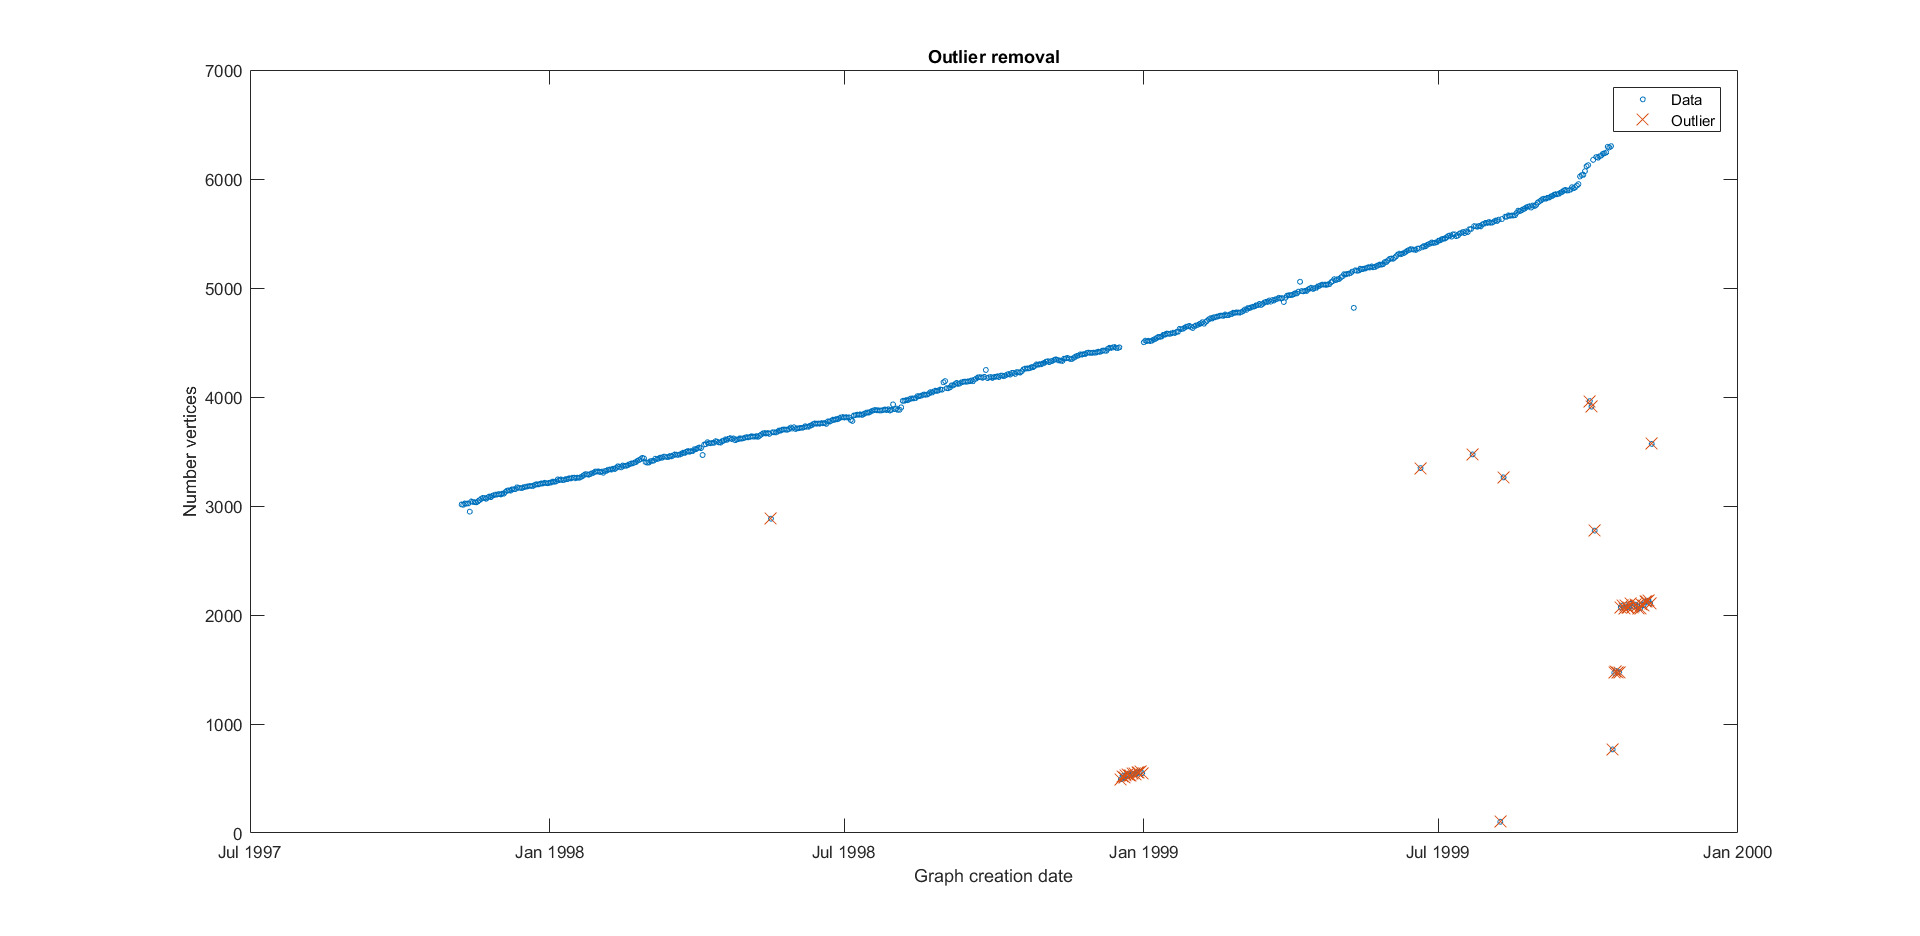
\includegraphics[width=\textwidth]{Outliers}
	\caption{Wykres liczby wierzchołków dla poszczególnych instancji z zaznaczonymi obserwacjami odstającymi}
\end{figure}



\chapter{Algorytmy}

\section{Centralność w grafach}

W teorii grafów wskaźniki centralności informują o najbardziej znaczących wierzchołkach grafu. Ich przykładowymi zastosowaniami mogą być: znalezienie lidera, przywódcy spośród danej grupy osób, ustalenie kluczowego elementu infrastruktury sieciowej lub miejskiej bądź znalezienie osobnika o największym potencjale do roznoszenia choroby. Istnieje wiele odmiennych wskaźników centralności. Zrealizowany projekt implementuje trzy z nich: Closeness Centrality, Betweenness Centrality oraz Pagerank ( jedna z odmian Eigenvector Centrality)



\section{Betweenness Centrality}

Określa kluczowość wierzchołka w zakresie komunikacji - przechodność, pośredniczenie. Czyli w jakim stopniu dany wierzchołek jest spoiwem dla danej sieci. Jest to miara o bardzo wielkiej wartości, gdyż dzięki niej można znaleźć punkty krytycznej sieci bądź grafu.

\subsection{Algorytm wyznaczania}
\begin{enumerate}
\item Wyznaczyć ilość najkrótszych ścieżek między wierzchołkami $u$ i $v$ ( $d_{uv}$ )
\item Wyznaczyć ilość najkrótszych ścieżek między wierzchołkami $u$ i $v$, które przechodzą przez wierzchołek $w$ ( $d_{uv}(w)$ )
\item Suma stosunków  oznacza stopień centralności wierzchołka $w$ $$c_b(w) = \sum_{u \neq v \neq w} \frac{d_{uv}(w)}{d_{uv}}$$
\end{enumerate}

\newpage
\FloatBarrier
\subsubsection{Przykład}
\begin{figure}[h]
\centering
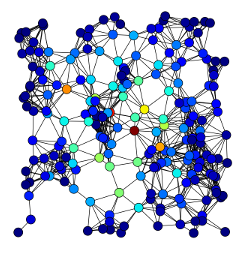
\includegraphics[scale=1.0]{betweenness_demo}
\caption{Działanie Betweenness Centrality  na przykładowym grafie}
\end{figure}
\FloatBarrier


\section{Closeness Centrality}

Jest to stopień bliskości. Określa jak blisko (daleko) wierzchołek ma do pozostałych w grafie. Wysoki stopień biskości świadczy o dobrej własności propagacji informacji w grafie - element ten szybko rozprowadzi daną wiadomość (wirusa itp) po całej sieci.


\subsubsection{Algorytm wyznaczania}
\begin{enumerate}
\item Wyznaczyć odległości pomiędzy wierzchołkiem $u$ a pozostałymi wierzchołkami w grafie $v$  ( $d_{uv}$ )
\item W zależności od rodzaju grafu zsumować otrzymane odległości:
\begin{enumerate}
\item Dla grafów rzadkich $$ c_c(u) = \frac{1}{\sum d_{uv} }$$
\item Dla grafów silnie połączonych $$ c_c(u) = \sum_{u \neq v} \frac{1}{d_{uv} }$$
\end{enumerate}
\end{enumerate}

\newpage
\FloatBarrier
\subsubsection{Przykład}
\begin{figure}[h]
\centering
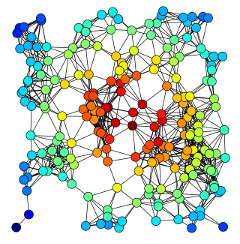
\includegraphics[scale=1.0]{closeness_demo}
\caption{Działanie Closeness Centrality  na przykładowym grafie}
\end{figure}
\FloatBarrier

\section{Eigenvector Centrality - Pagerank}
Określa wpływ, oddziaływanie wierzchołka na pozostałe w grafie. Wykorzystuje nie tylko ilość połączeń danego wierzchołka z innymi, a przede wszystkim ich jakość. Wartości przypisane do każdego z wierzchołków bazują na koncepcji w której wysoko ocenione wierzchołki bardziej wpływają na ostateczną ocenę połączonego wierzchołka, niż te, których ocena jest niska. Jedną z odmian Eigenvector Centrality jest algorytm PageRank. Poniżej przedstawiono uproszczony algorytm jego działania.

\subsubsection{Algorytm wyznaczania}
\begin{enumerate}
\item Wyznaczyć ilość wierzchołków w grafie ($N$)
\item Wyznaczyć stopień każdego z wierzchołków ($l(u)$)
\item Zainicjować wartości początkowe dla każdego wierzchołka wartością początkową ($c_e(u) = 1$)
\item Określić współczynnik tłumienia, zwykle wynosi on około 0.85 ( $d = 0.85$ )
\item Obliczyć nową wartość PageRank każdego wierzchołka $$ c_e(u) = \frac{1 - d}{N} + d\sum_{v \in B_u} \frac{c_e(v)}{l(v)}$$ $B_u$ oznacza zbiór wszystkich wierzchołków, które odnoszą się do wierzchołka $u$
\end{enumerate}

\newpage
\FloatBarrier
\subsubsection{Przykład}
\begin{figure}[h]
\centering
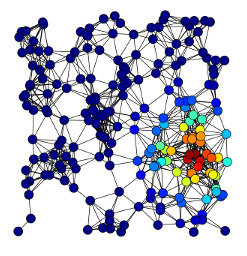
\includegraphics[scale=1.0]{pagerank_demo}
\caption{Działanie Eigenvector Centrality  na przykładowym grafie}
\end{figure}
\FloatBarrier
\newpage
\FloatBarrier
\section{Ogólne charakterystyki grafów}
\FloatBarrier
\subsection{Podstawowe miary}
\begin{figure}[h]
	\centering
	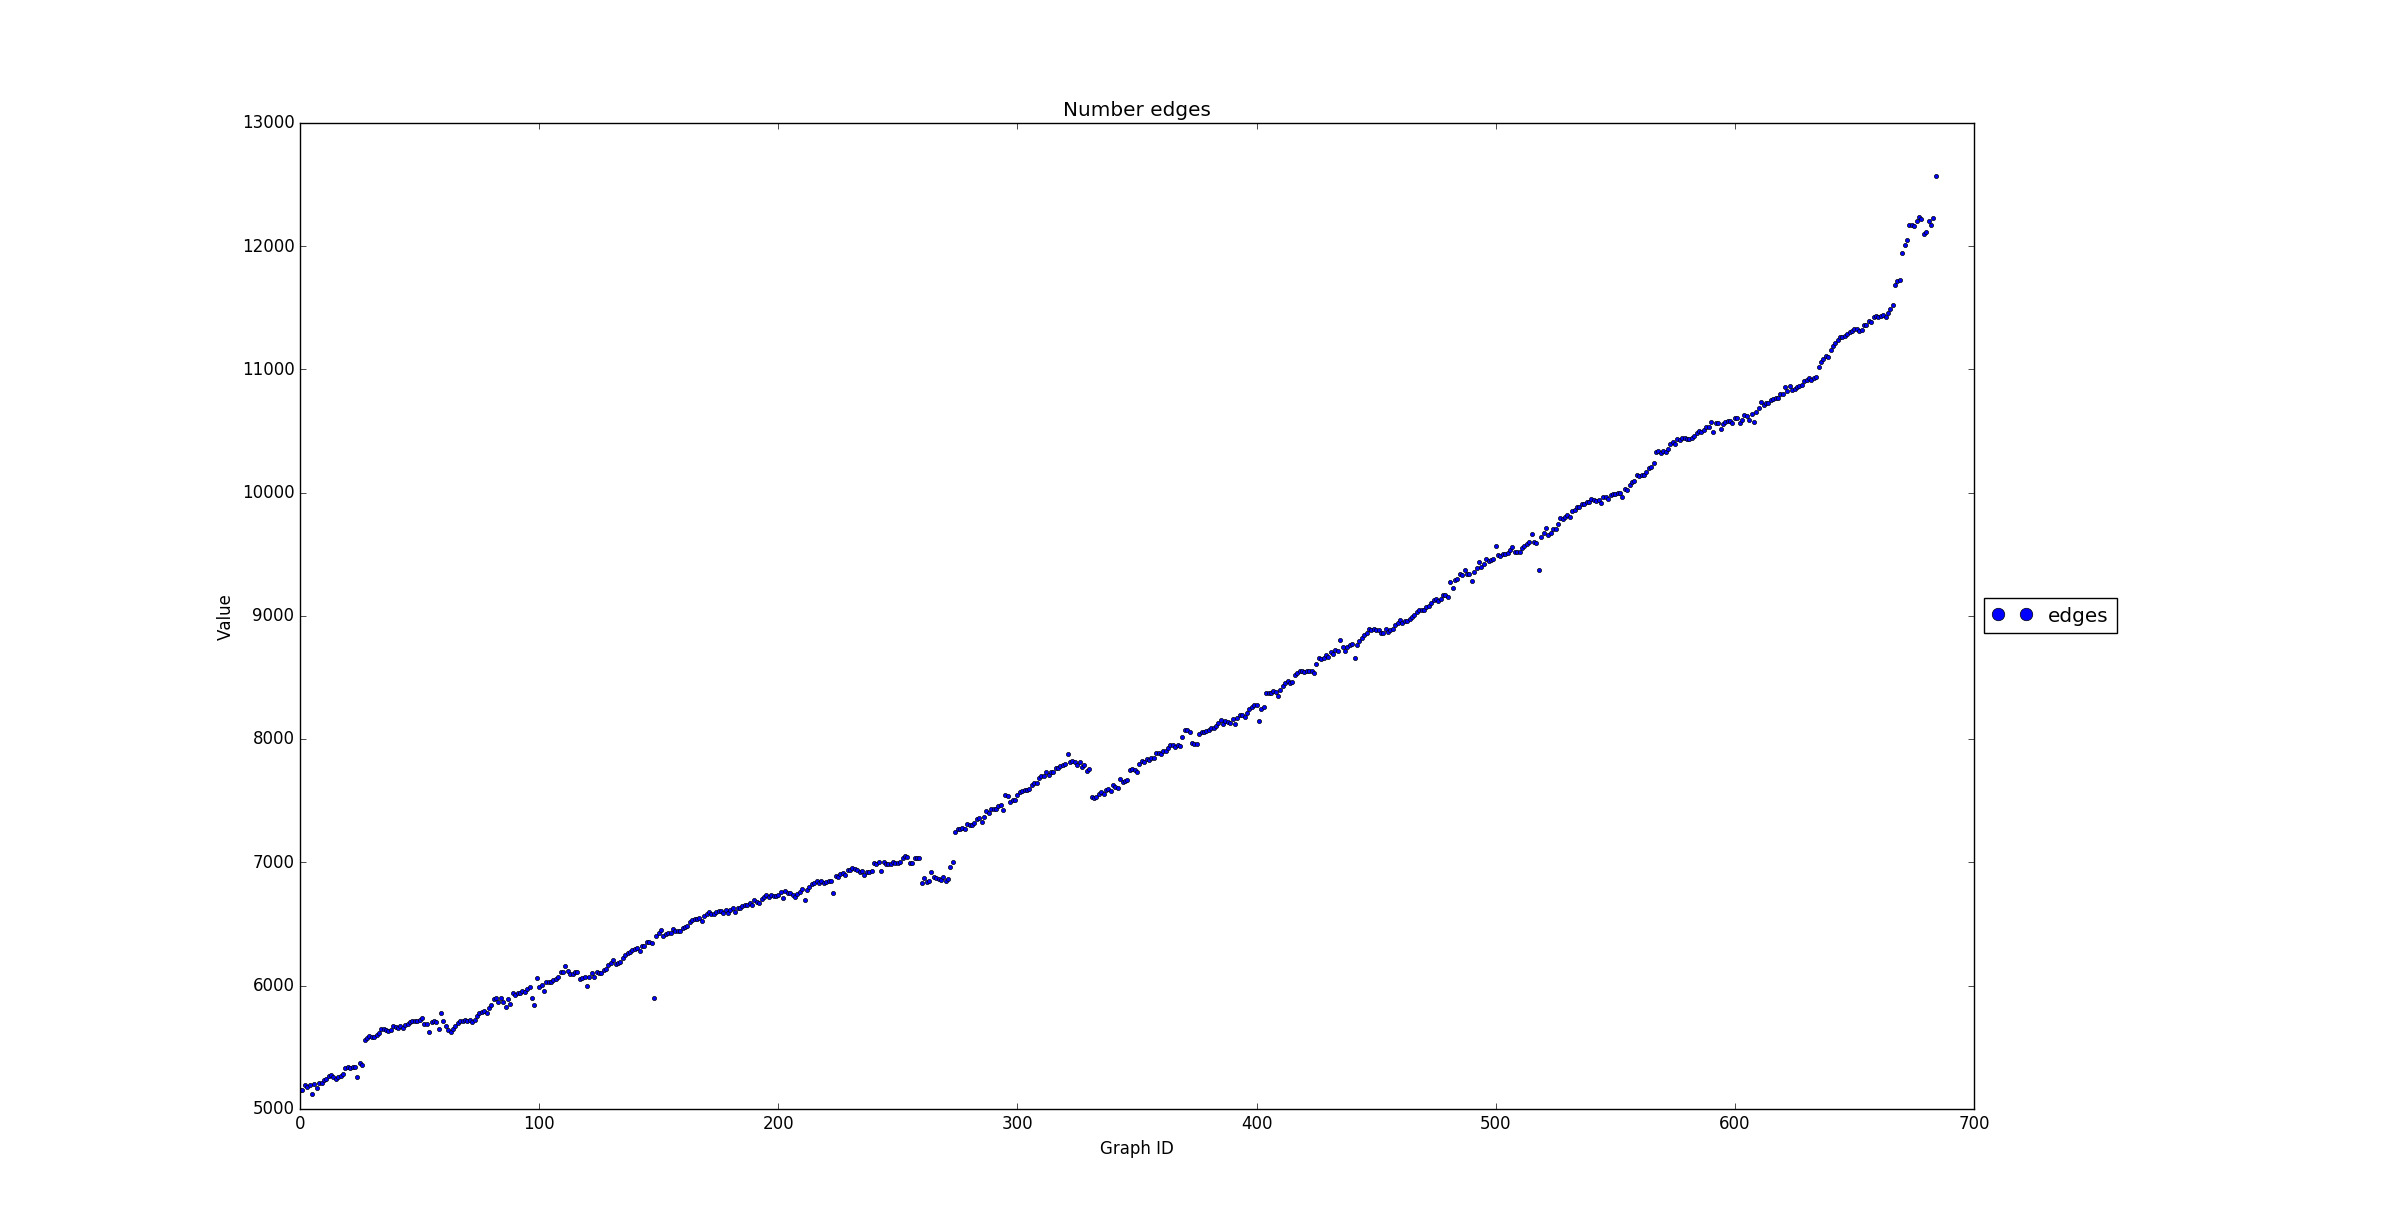
\includegraphics[width=\textwidth]{number_edges}
	\caption{Ilość krawędzi w sieci}
\end{figure}
\FloatBarrier
\FloatBarrier
\begin{figure}[h]
	\centering
	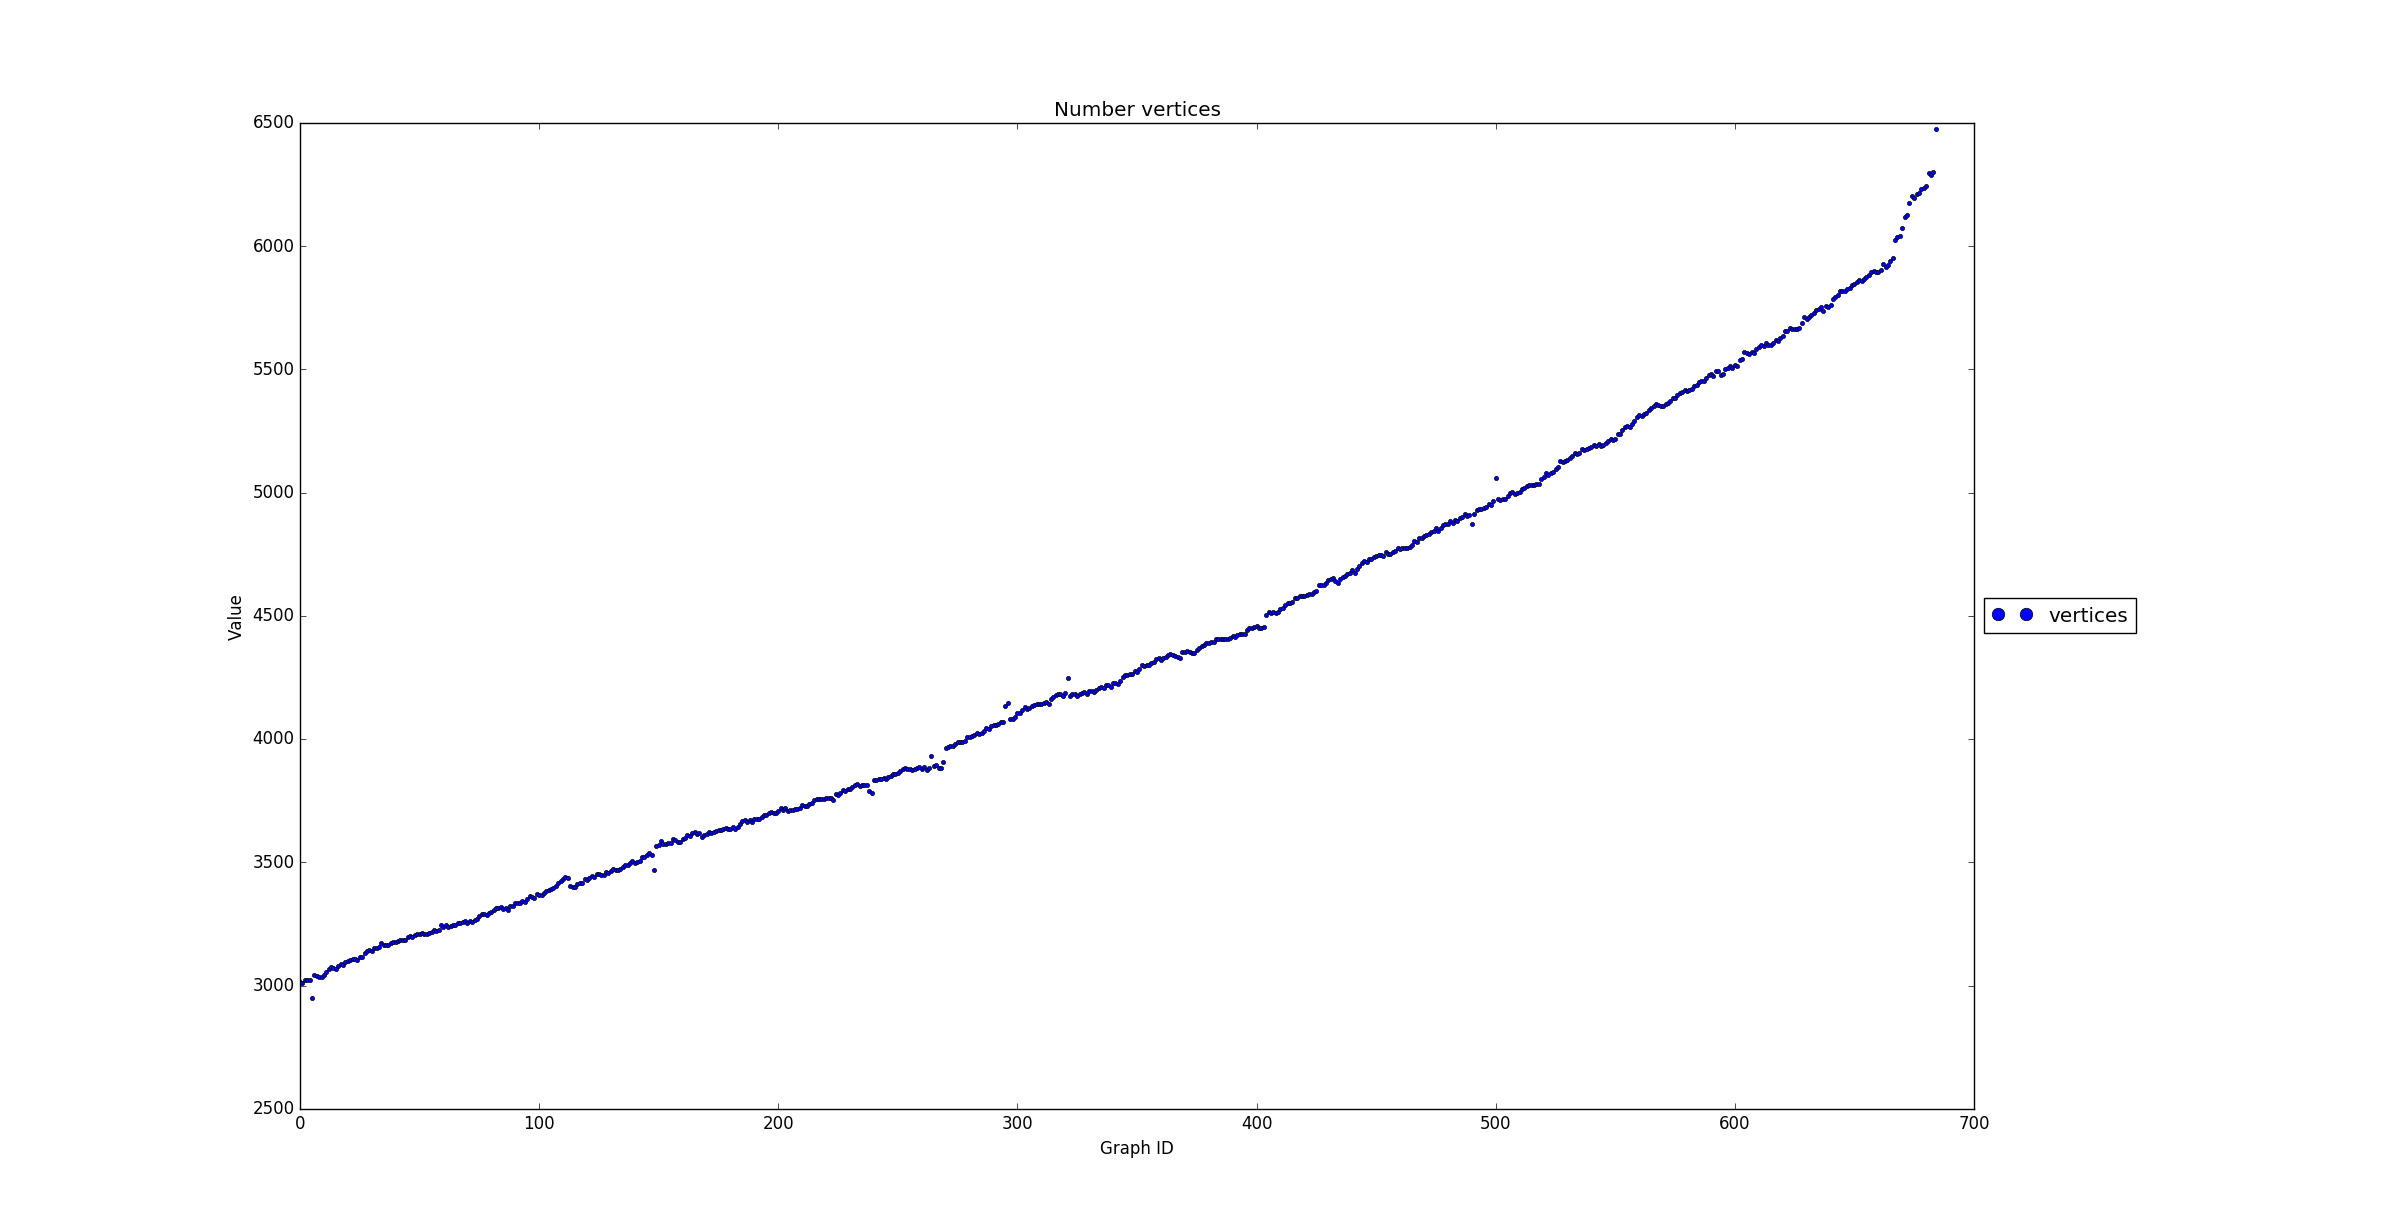
\includegraphics[width=\textwidth]{number_vertices}
	\caption{Ilość wierzchołków w sieci}
\end{figure}
\FloatBarrier
\FloatBarrier
\begin{figure}[h]
	\centering
	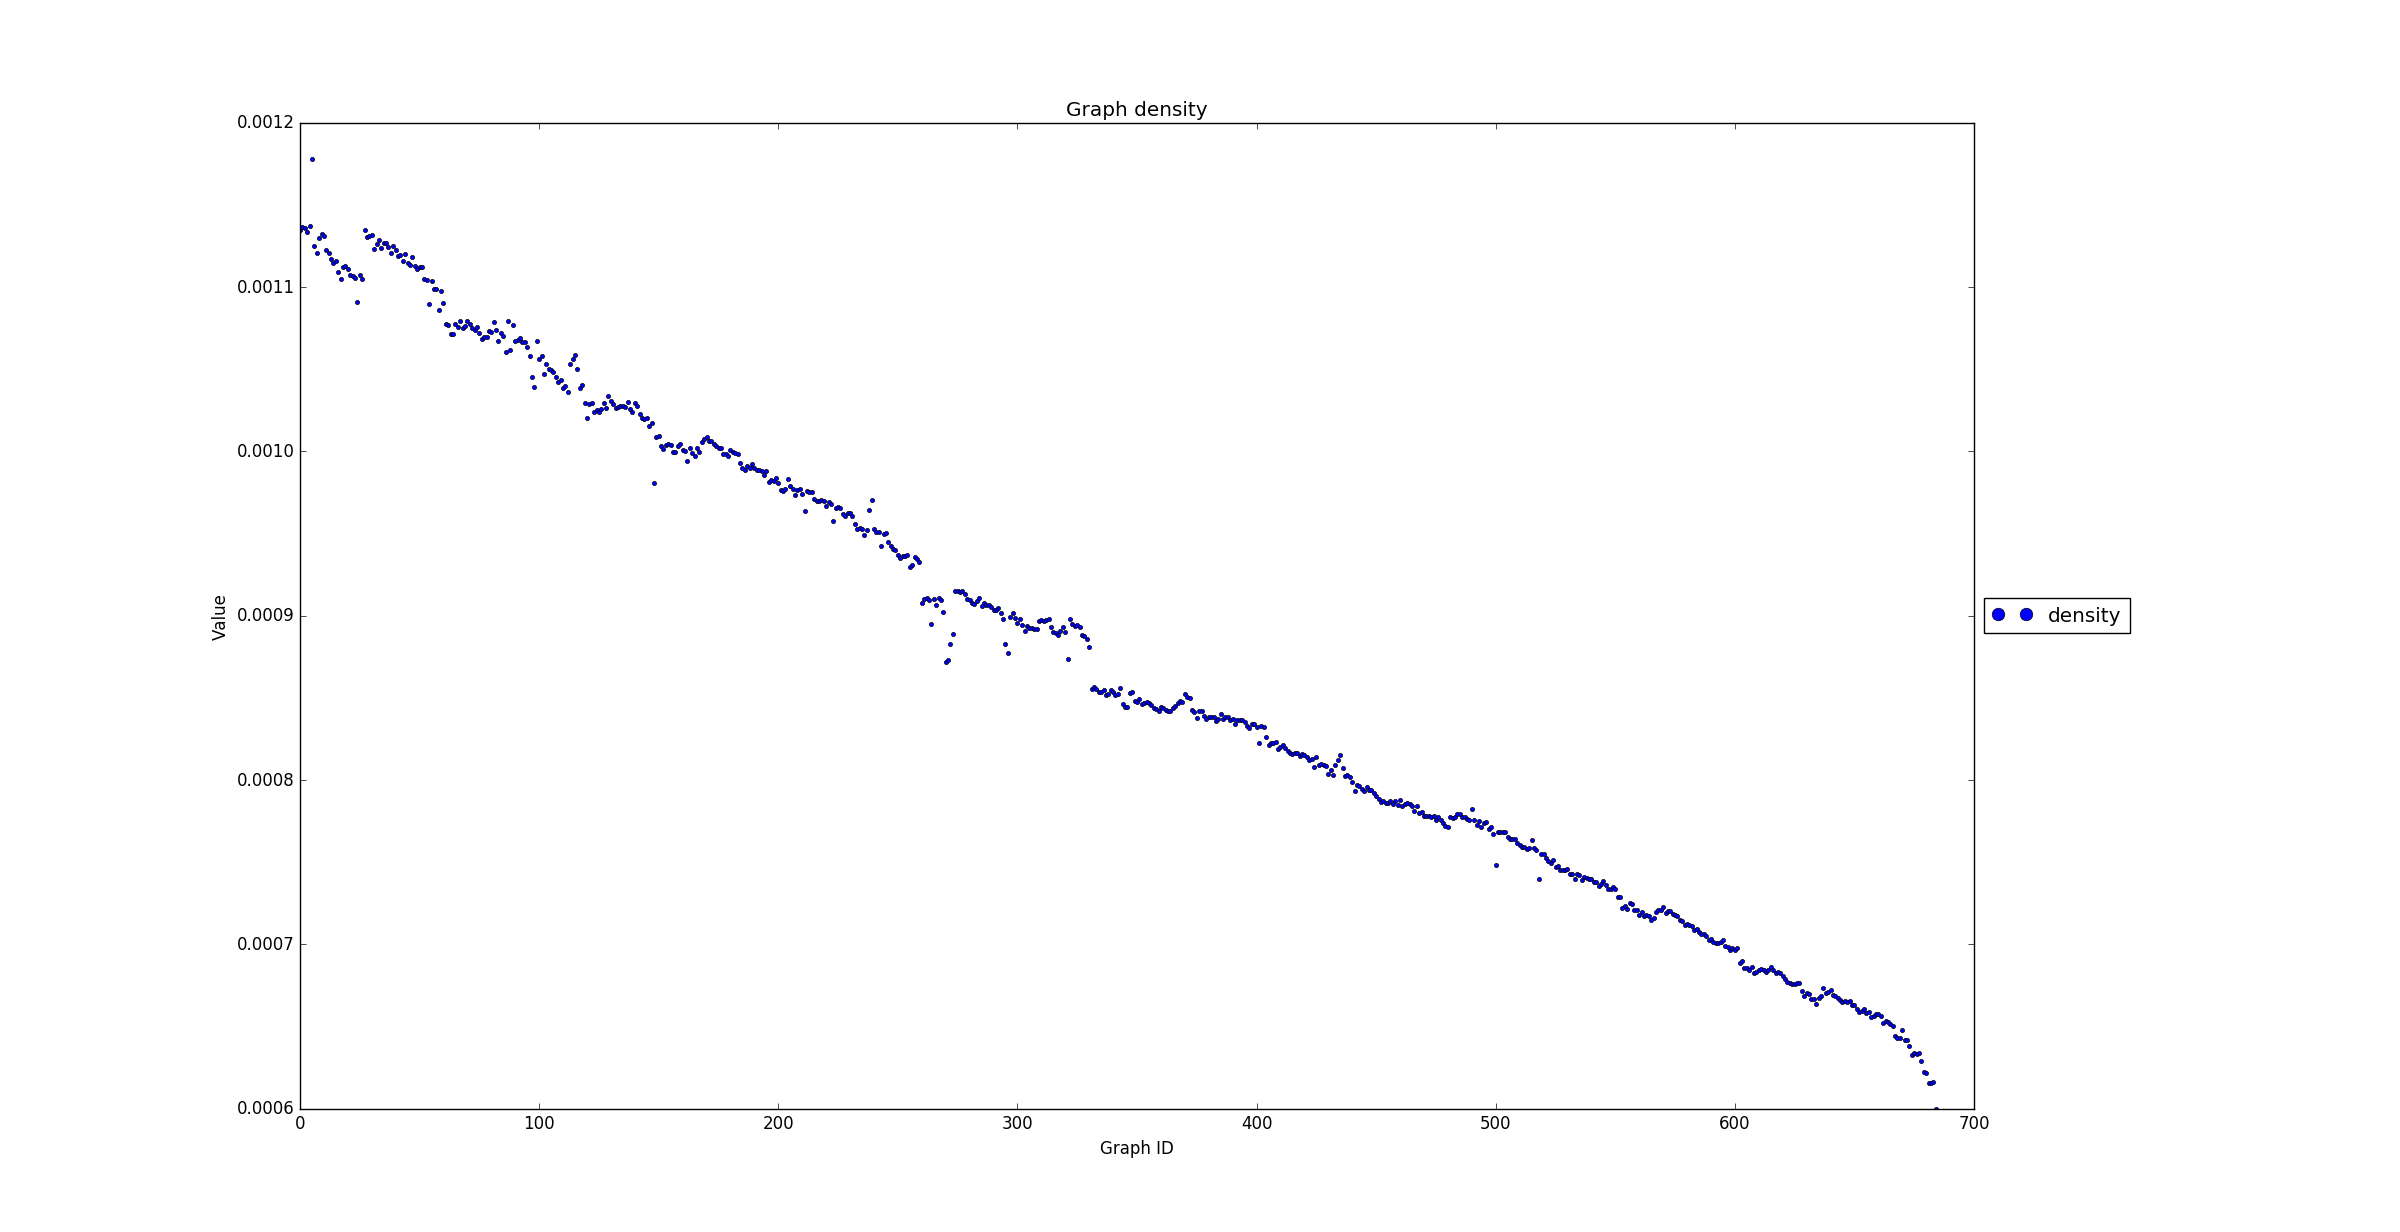
\includegraphics[width=\textwidth]{graph_density}
	\caption{Gęstość grafu}
\end{figure}
\FloatBarrier
Malejąca gęstość grafu wynika wprost z tego, że stosunek ilości wierzchołków do krawędzi jest stały w miarę upływu czasu, mimo tego że obie wartości rosną. Gęstość grafu liczymy ze wzoru:
\begin{equation}
\label{graph_density}
d=\frac{2m}{n(n-1)}
\end{equation}
$d$ - gęstość grafu, 
$m$ - ilość krawędzi, 
$n$ - ilość wierzchołków

Da się łatwo zauważyć, że jeśli stosunek $\frac{m}{n} = const$, a w tym przypadku $\frac{m}{n} \approx 2 \Rightarrow m \approx 2n$ to wzór \ref{graph_density} można zapisać następująco:
\begin{equation}
\label{graph_density_simplified}
d \approx \frac{4n}{n(n-1)} \equiv d \approx \frac{4}{n-1}
\end{equation}

Jak widać po przekształceniu uzyskujemy hiperbolę, którą dla dużych $n$ na wąskim przedziale $[3000, 6500]$ można przybliżyć malejącą funkcją liniową.
\FloatBarrier
\newpage
\FloatBarrier
\section{Miary dla wierzchołków}
\begin{figure}[h]
	\centering
	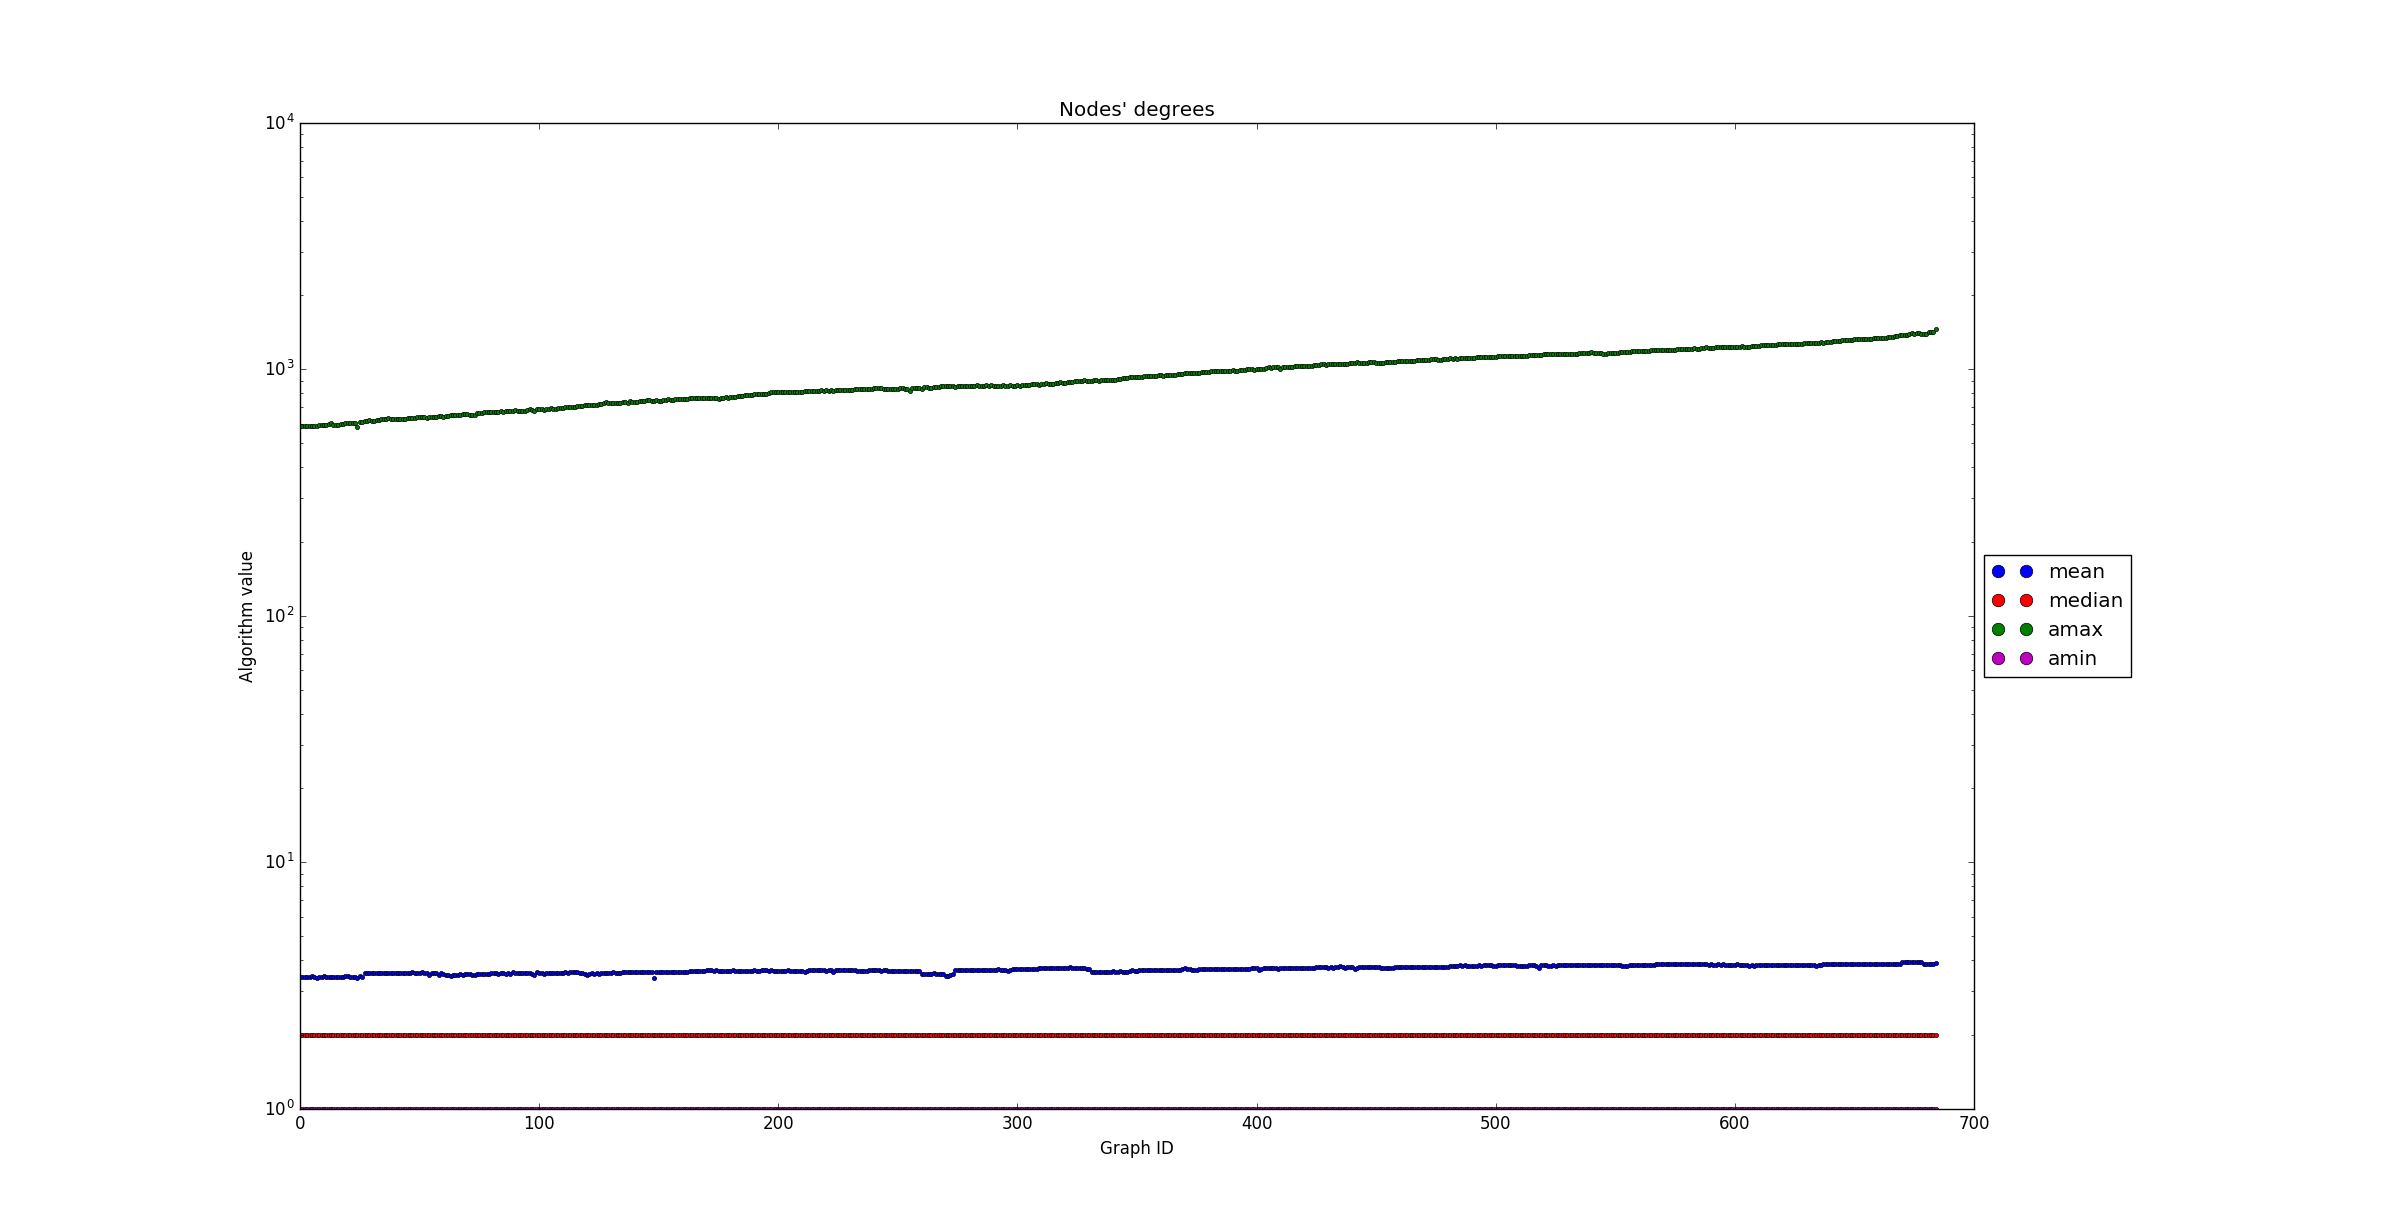
\includegraphics[width=\textwidth]{nodes_degrees}
	\caption{Stopnie wierzchołków}
\end{figure}
\FloatBarrier
\FloatBarrier
\begin{figure}[h]
	\centering
	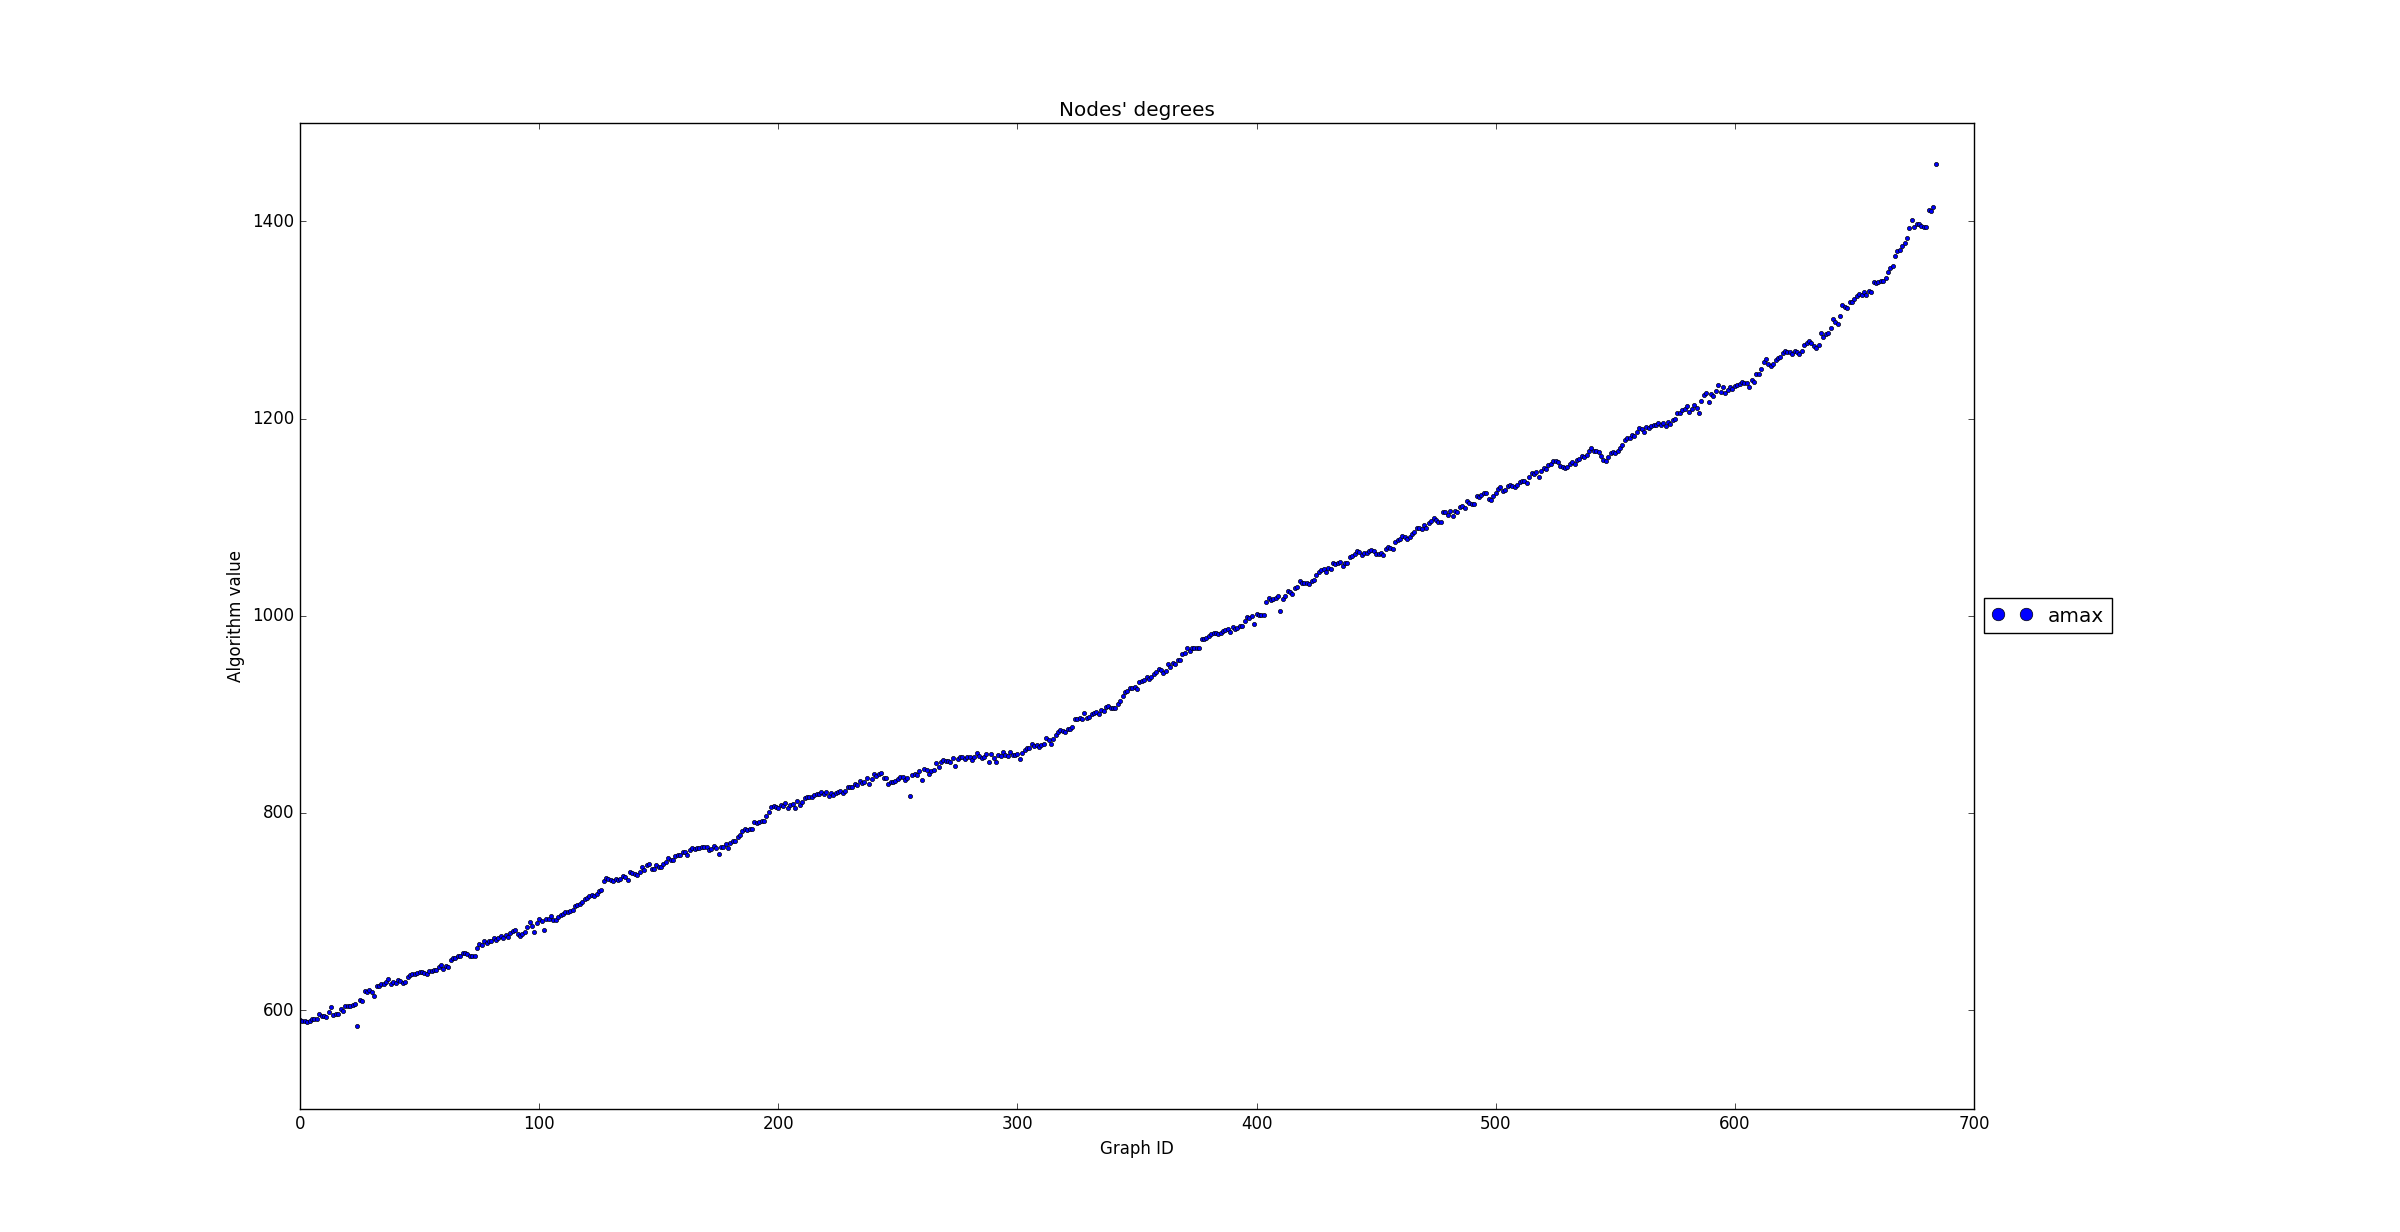
\includegraphics[width=\textwidth]{nodes_degree_max}
	\caption{Maksymalne stopnie wierzchołków }
\end{figure}
\FloatBarrier
\FloatBarrier
\begin{figure}[h]
	\centering
	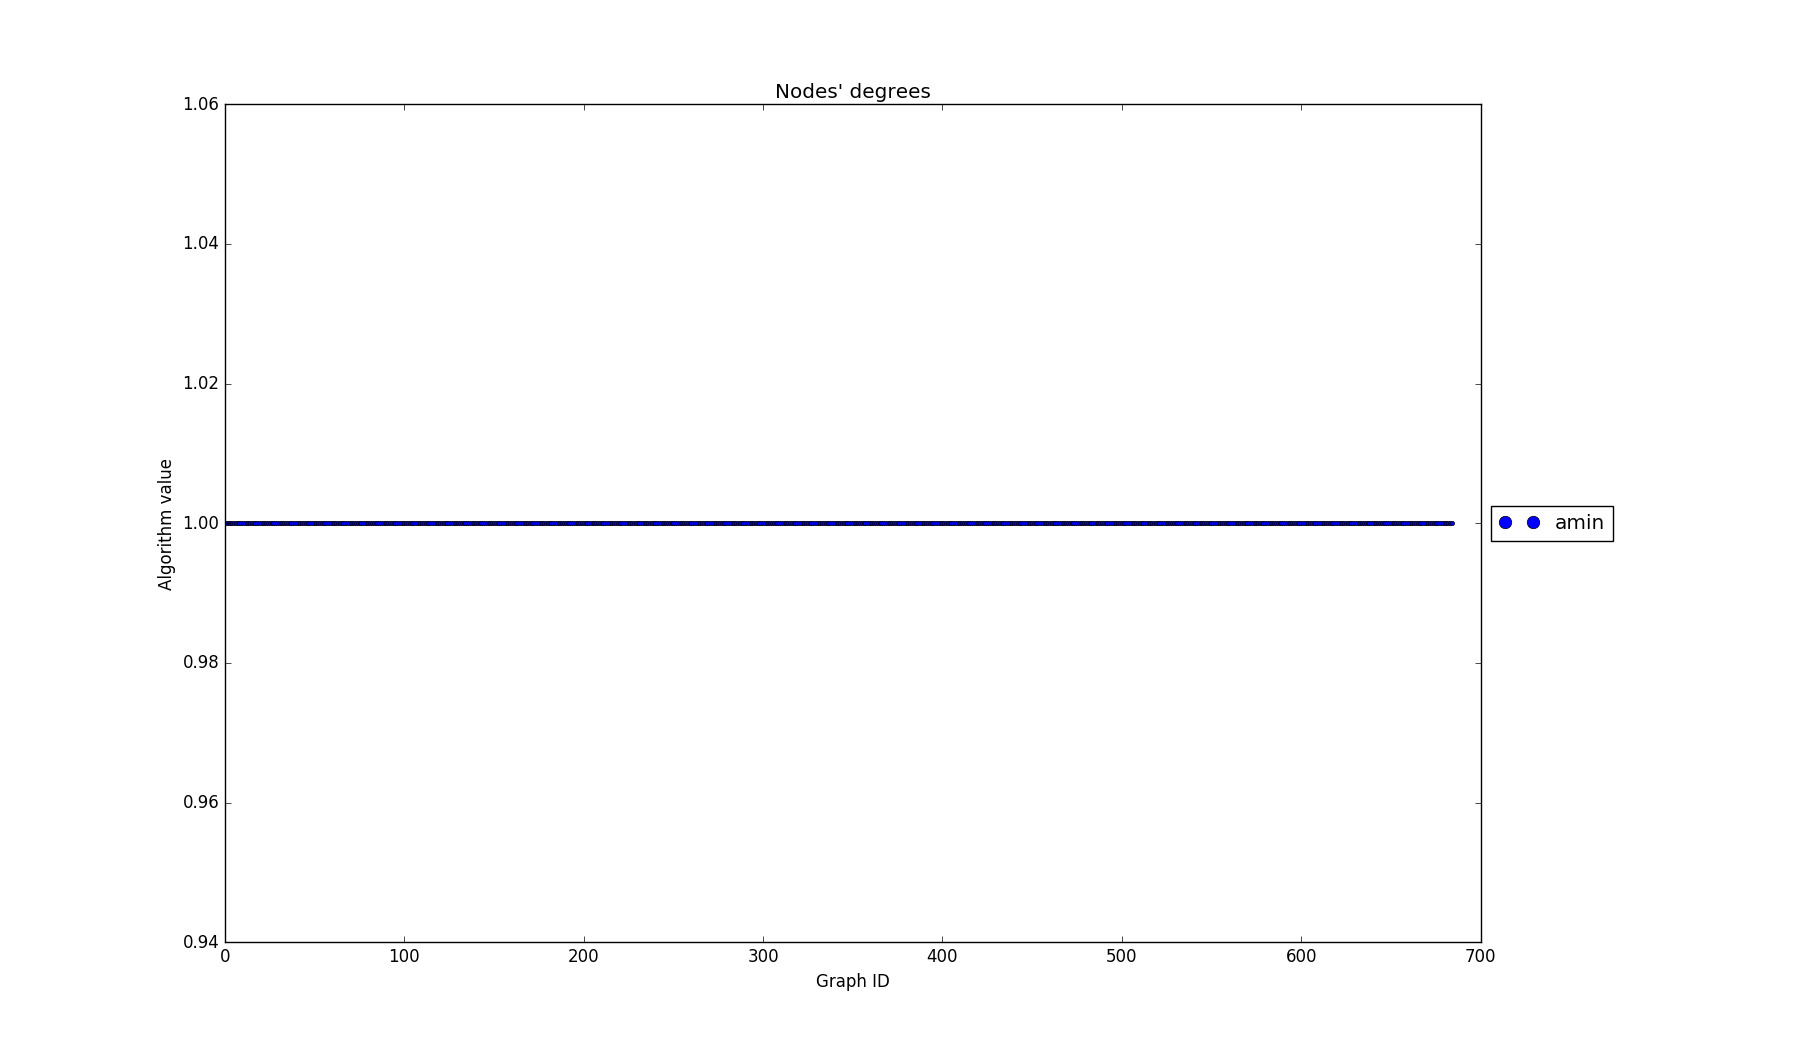
\includegraphics[width=\textwidth]{nodes_degree_min}
	\caption{Minimalne stopnie wierzchołków}
\end{figure}
\FloatBarrier\FloatBarrier
\begin{figure}[h]
	\centering
	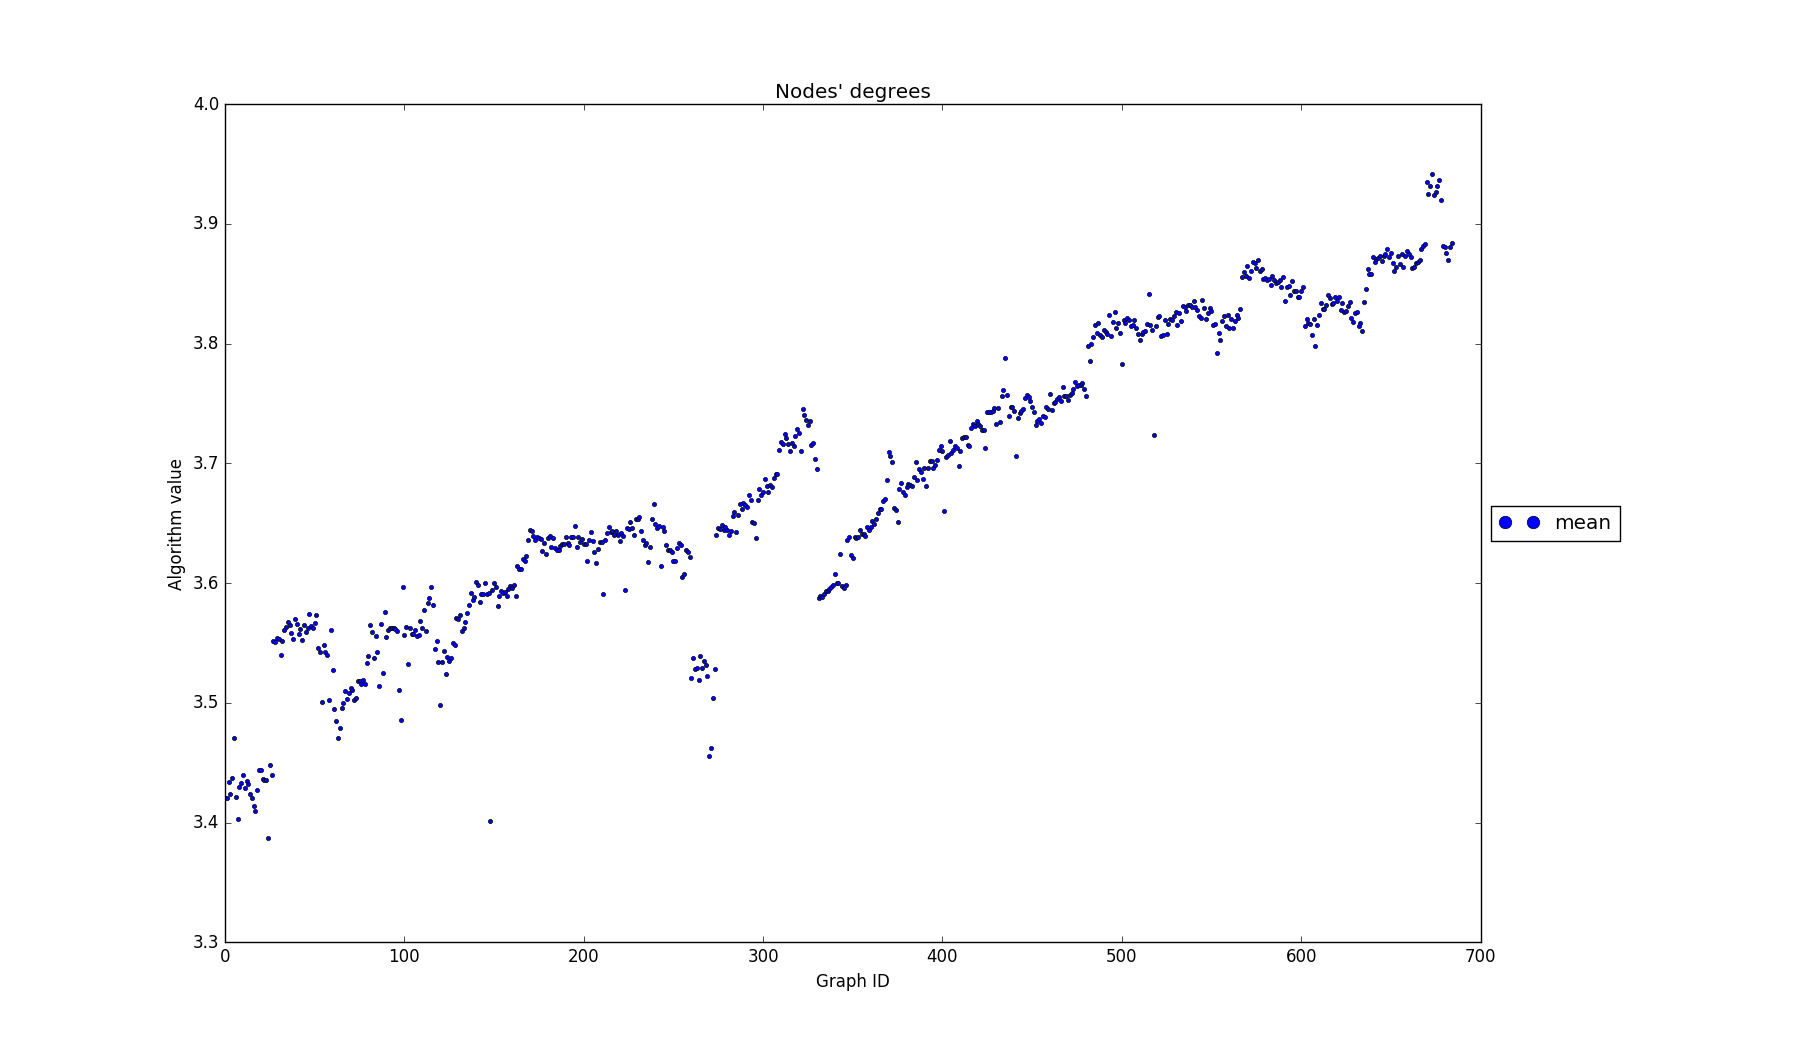
\includegraphics[width=\textwidth]{nodes_degrees_mean}
	\caption{Średni stopień wierzchołka w grafie}
\end{figure}
\FloatBarrier\FloatBarrier
\begin{figure}[h]
	\centering
	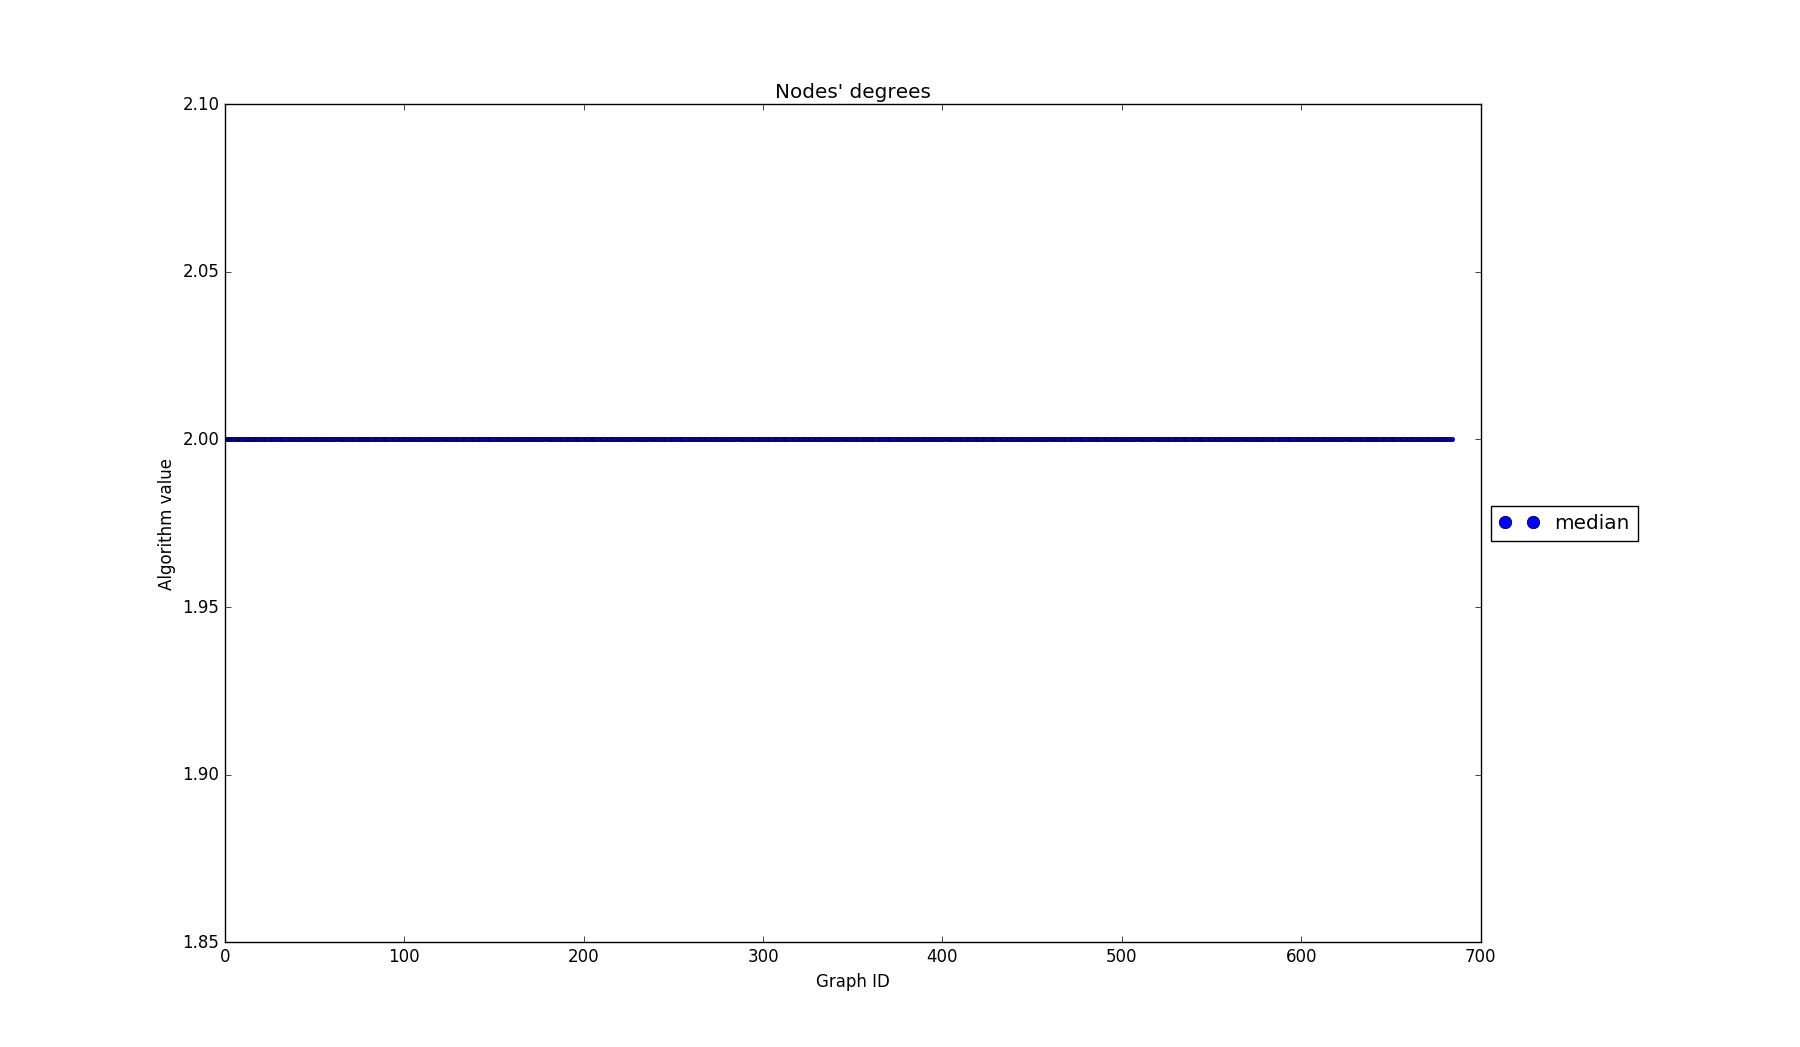
\includegraphics[width=\textwidth]{nodes_degrees_median}
	\caption{Mediana stopni wierzchołka}
\end{figure}
\FloatBarrier\FloatBarrier
\begin{figure}[h]
	\centering
	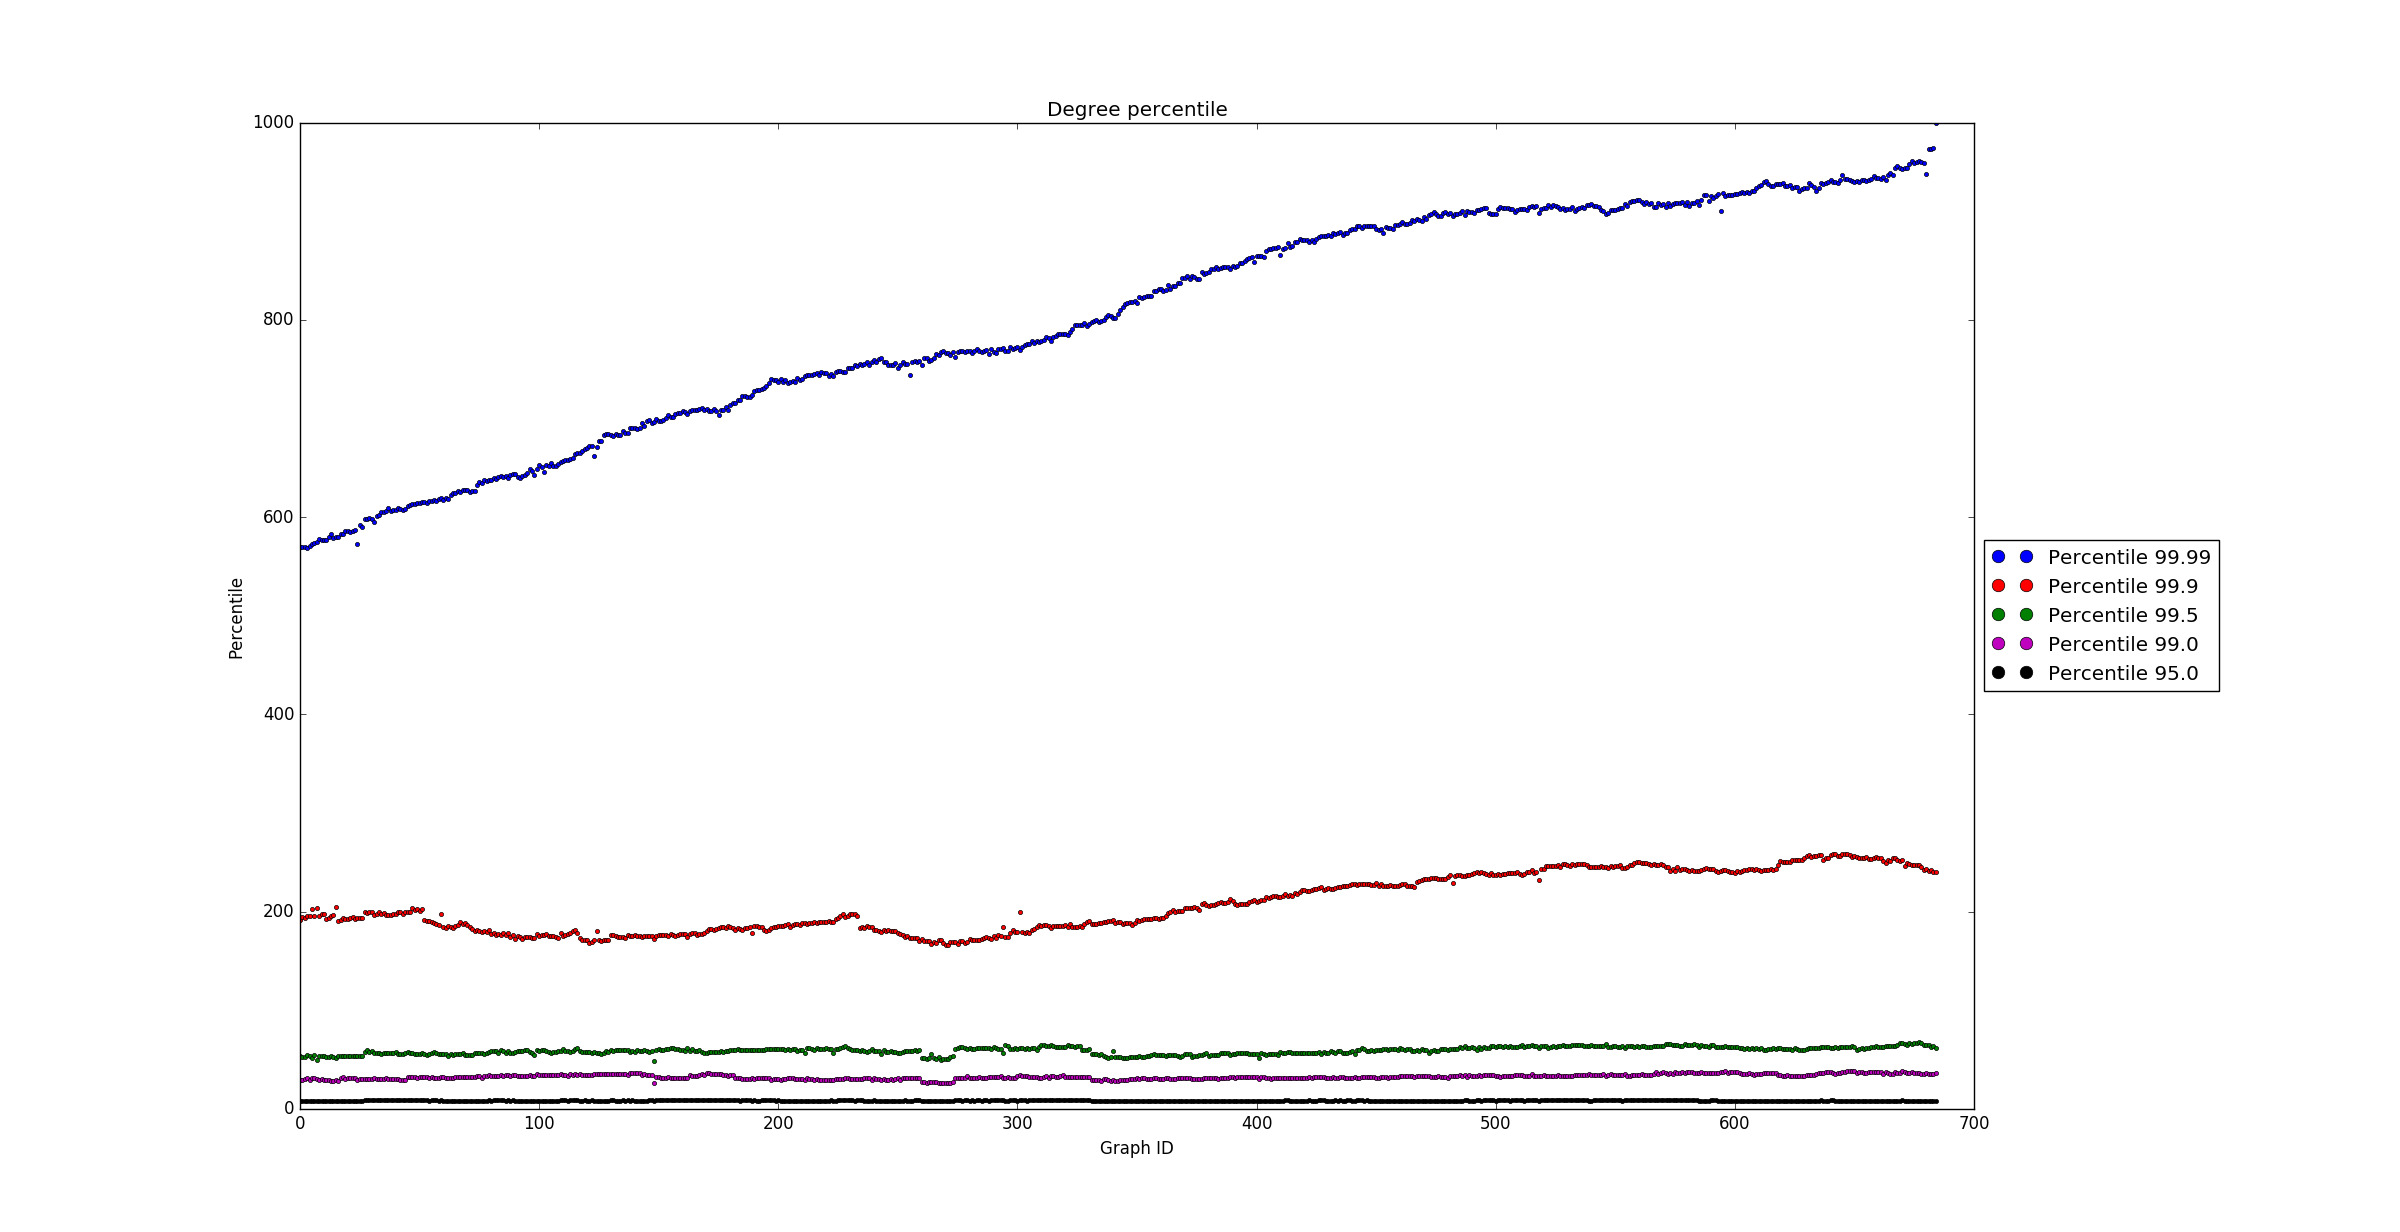
\includegraphics[width=\textwidth]{degree_percentiles}
	\caption{Percentyle dla stopni wierzchołka}
\end{figure}

Z powyższych wykresów wynika, że graf jest duży i ma relatywnie niską gęstość połączeń. Przez cały okres duża ilość wierzchołków (95\%) ma niski stopień, co przekłada się na niską średnią oraz medianę i może wpływać na wyniki algorytmów. 
\FloatBarrier\FloatBarrier
\newpage
\subsubsection{Przykład}
\begin{figure}[h]
	\centering
	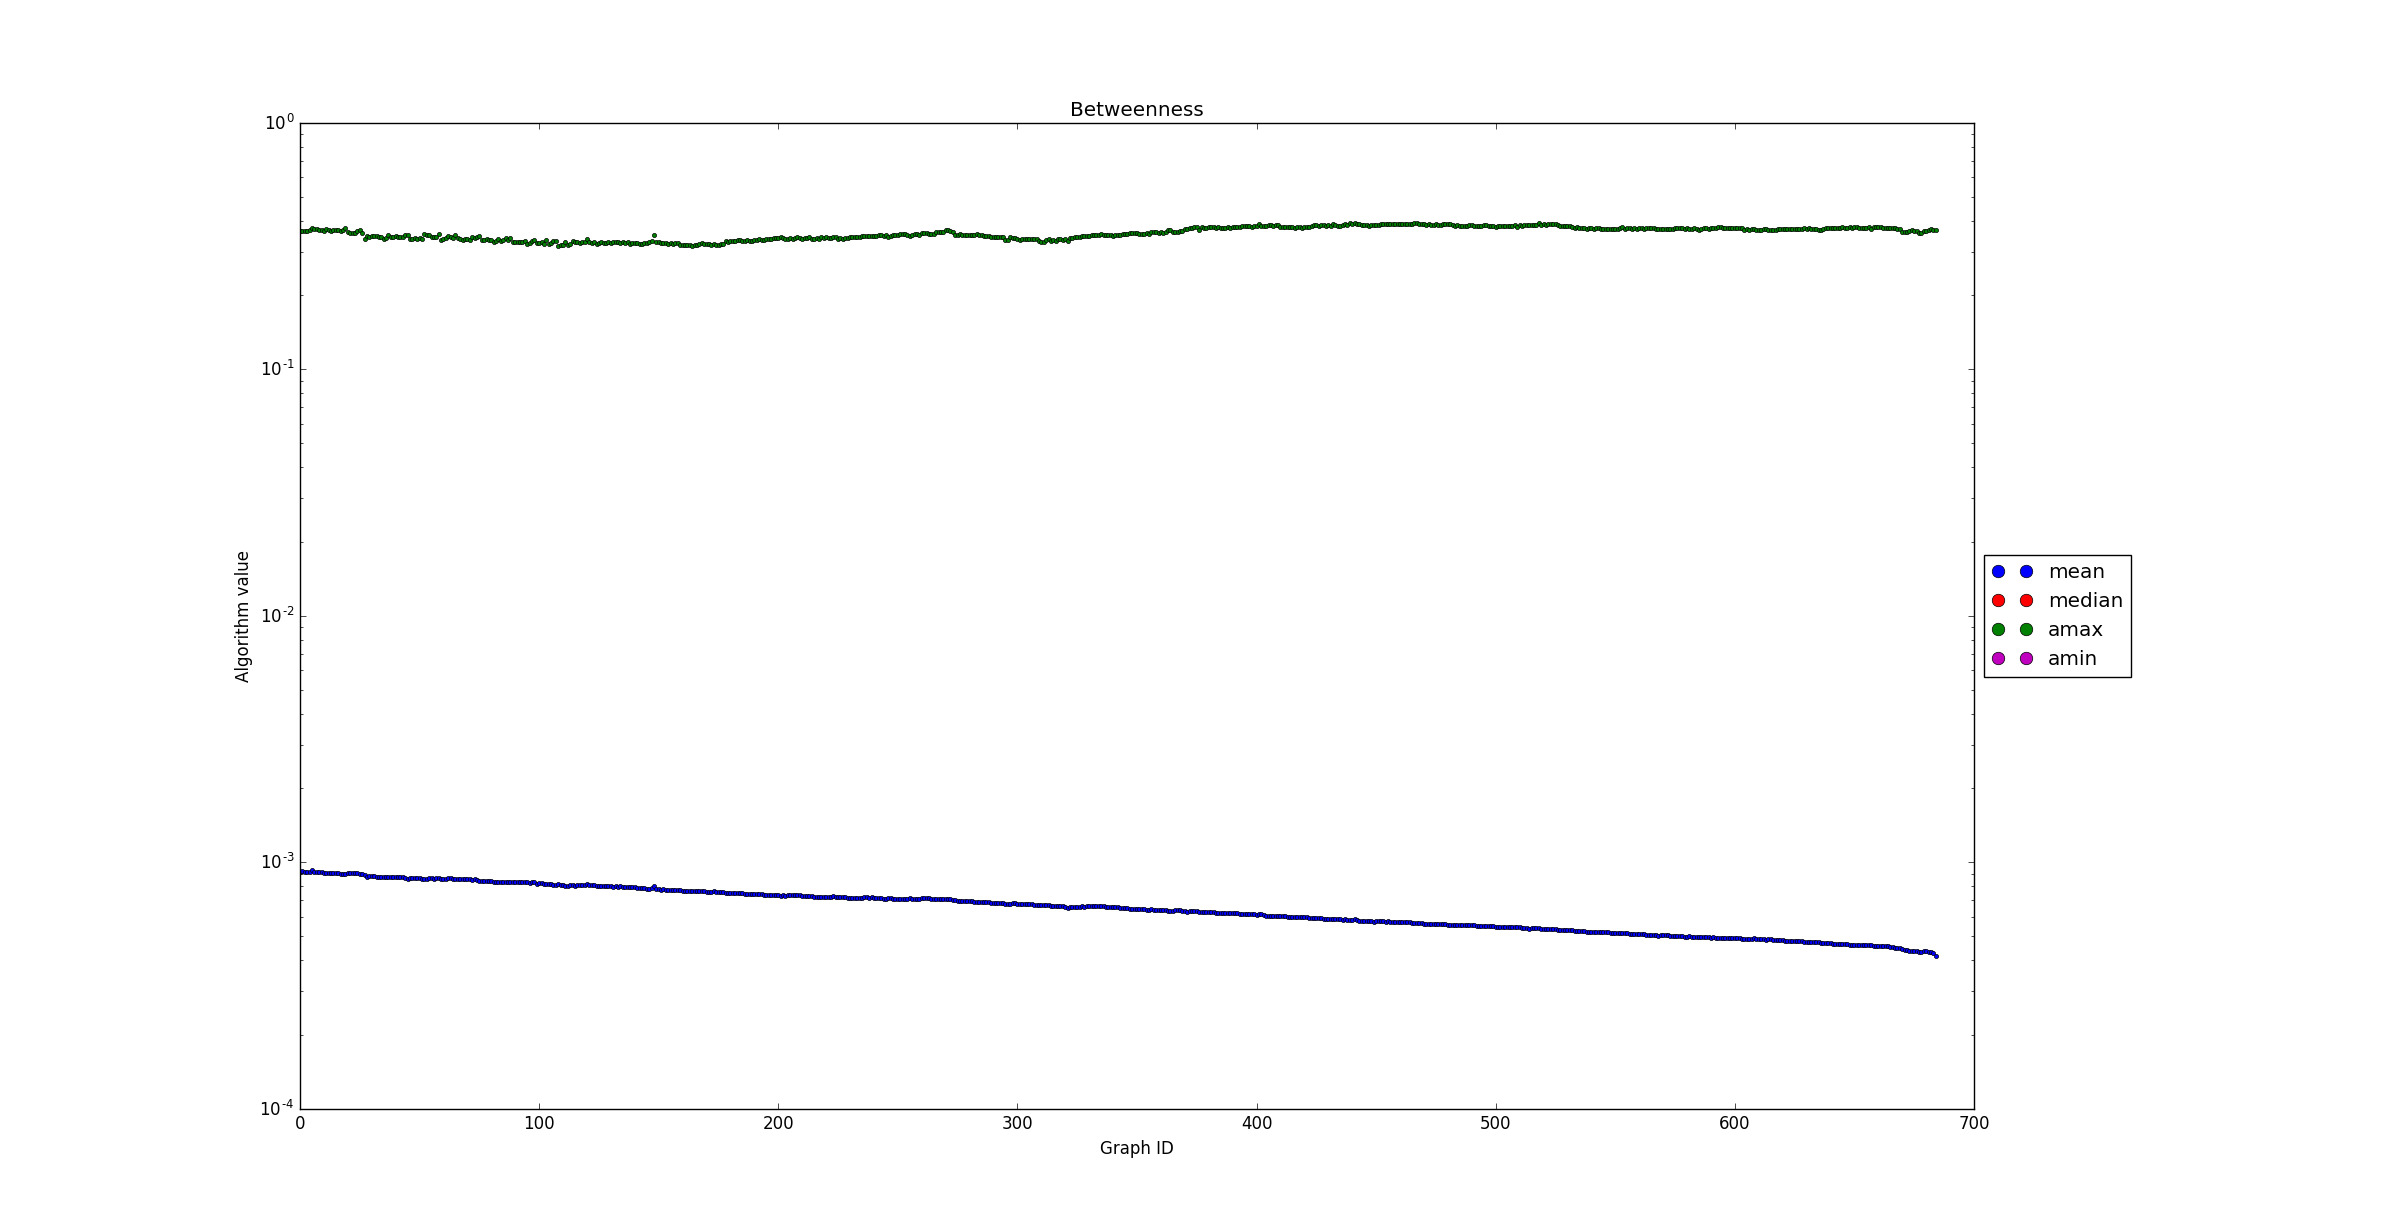
\includegraphics[width=\textwidth]{betweenness}
	\caption{Działanie Betweenness Centrality  na przykładowym grafie}
\end{figure}
\FloatBarrier
\subsubsection{Przykład}
\begin{figure}[h]
	\centering
	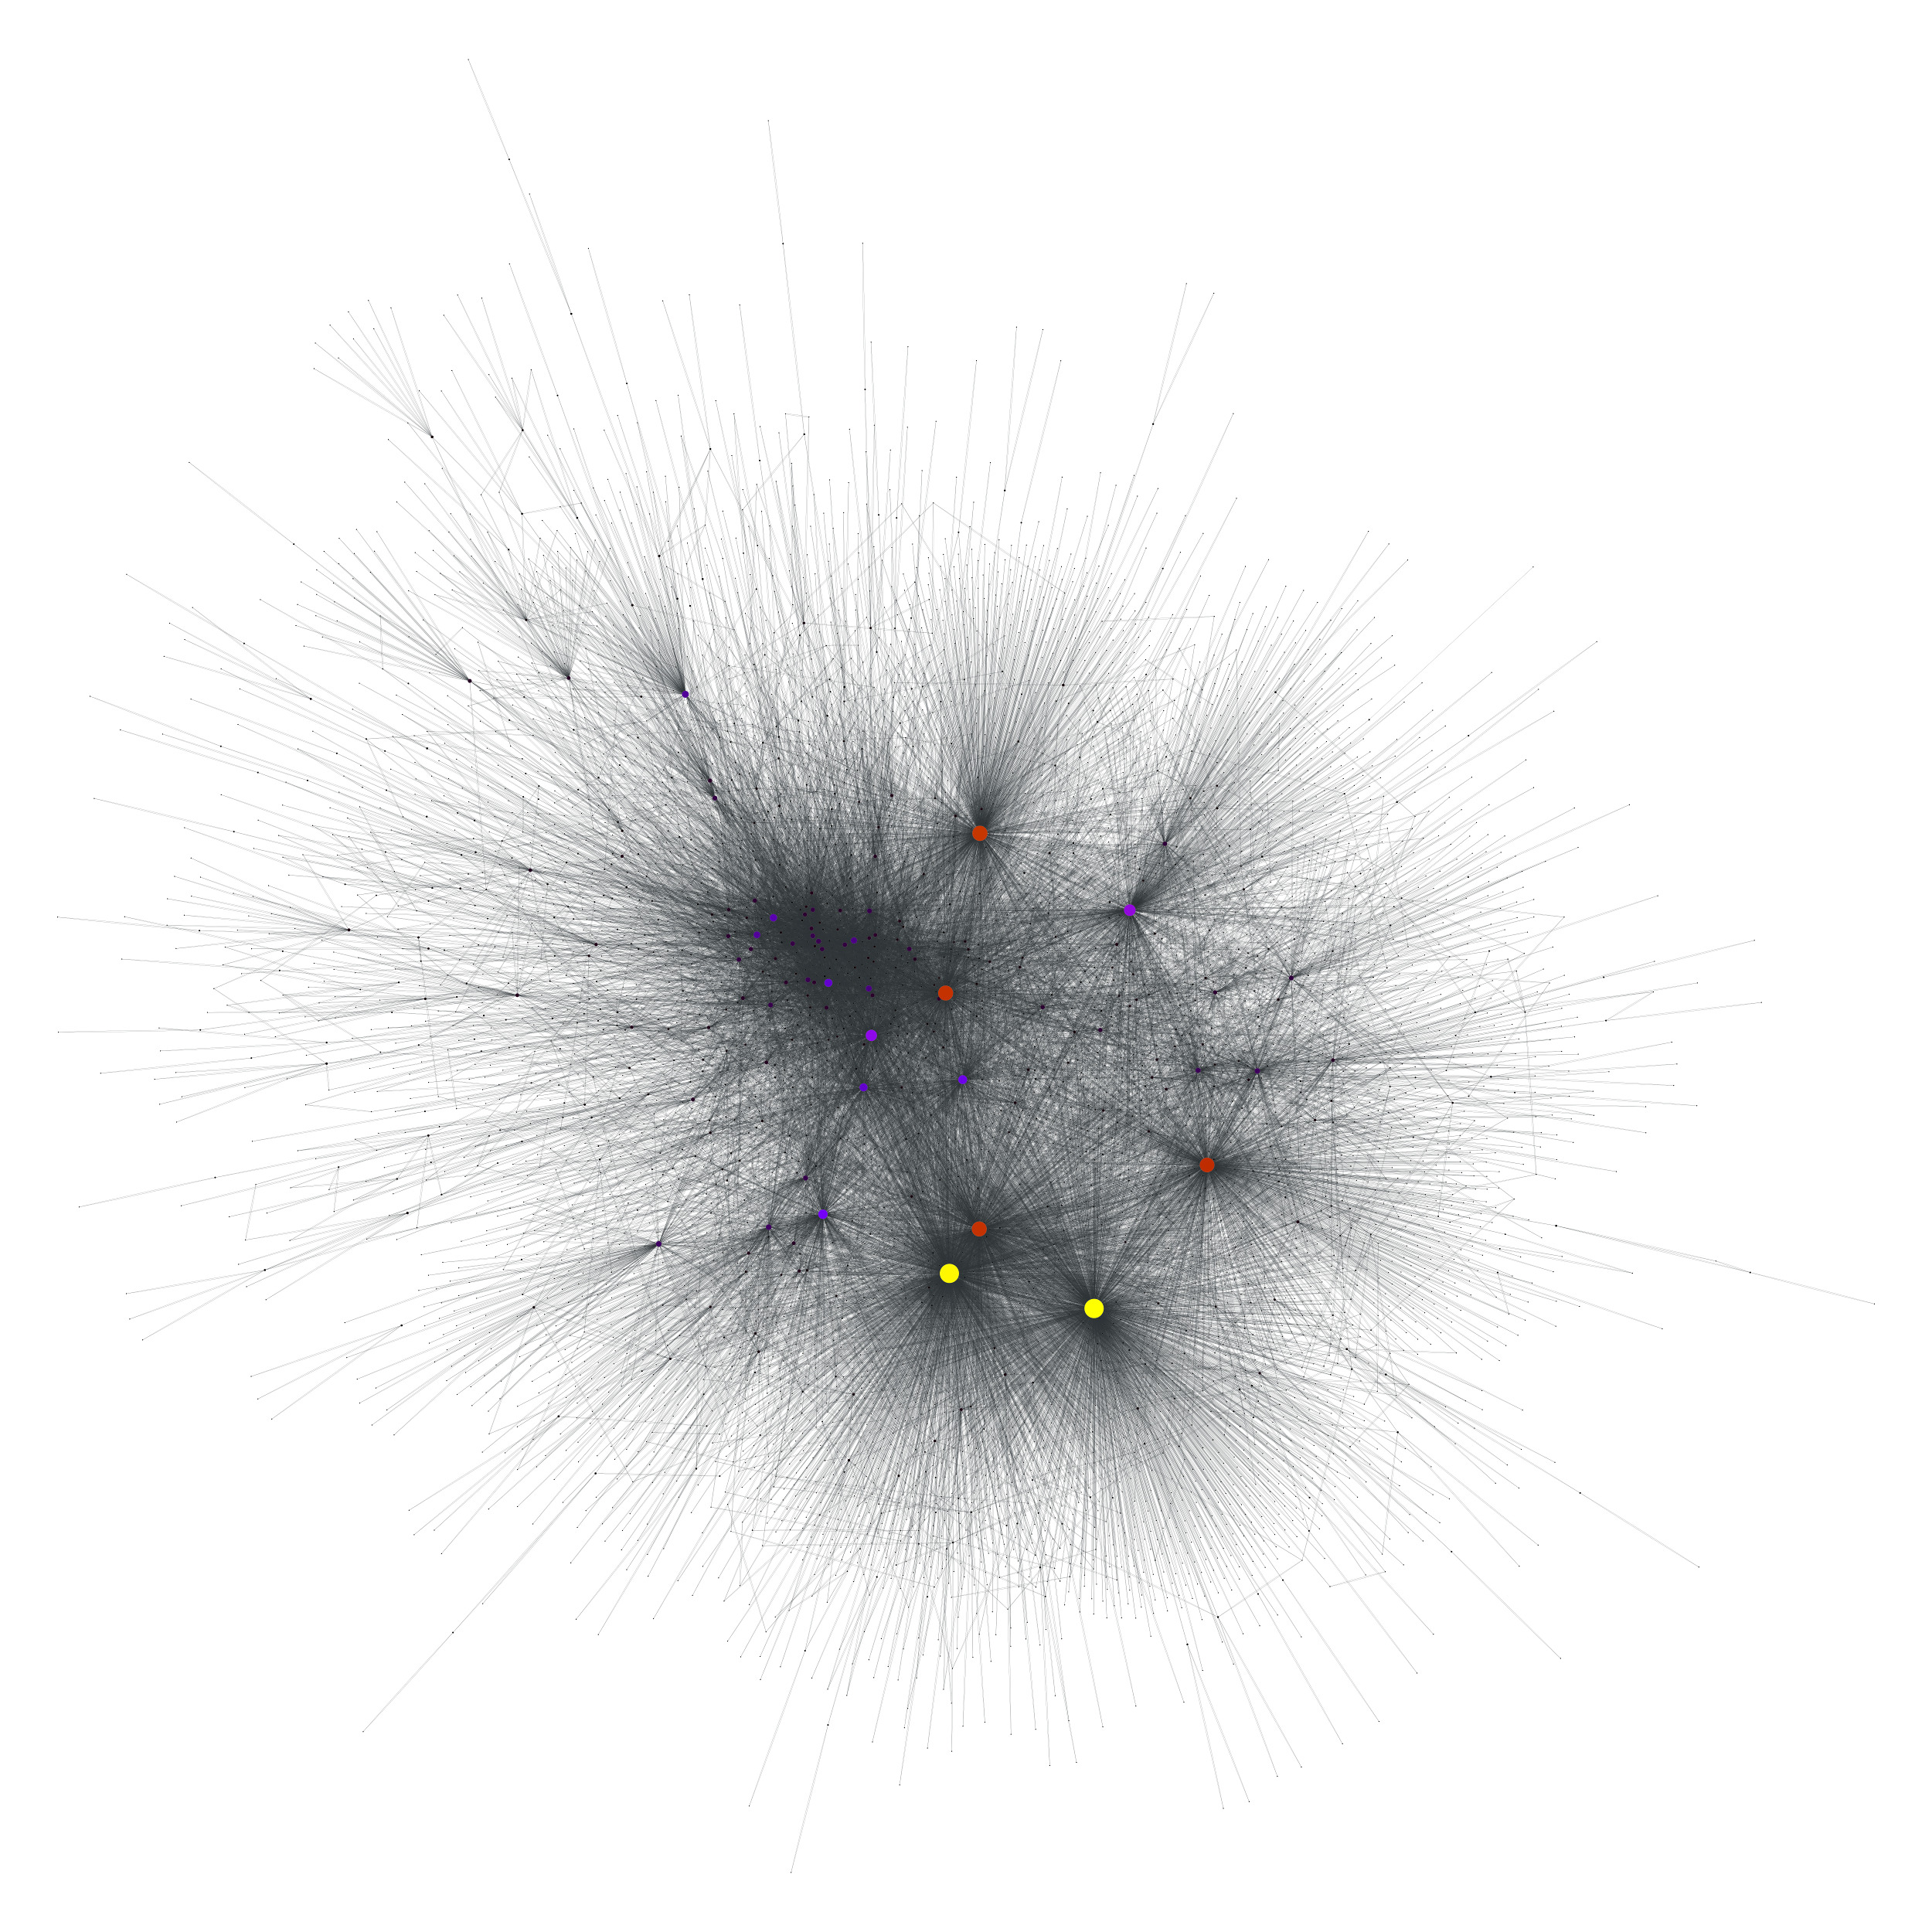
\includegraphics[width=\textwidth]{betweenness_8k}
	\caption{Działanie Betweenness Centrality  na przykładowym grafie}
\end{figure}
\FloatBarrier
\subsubsection{Przykład}
\begin{figure}[h]
	\centering
	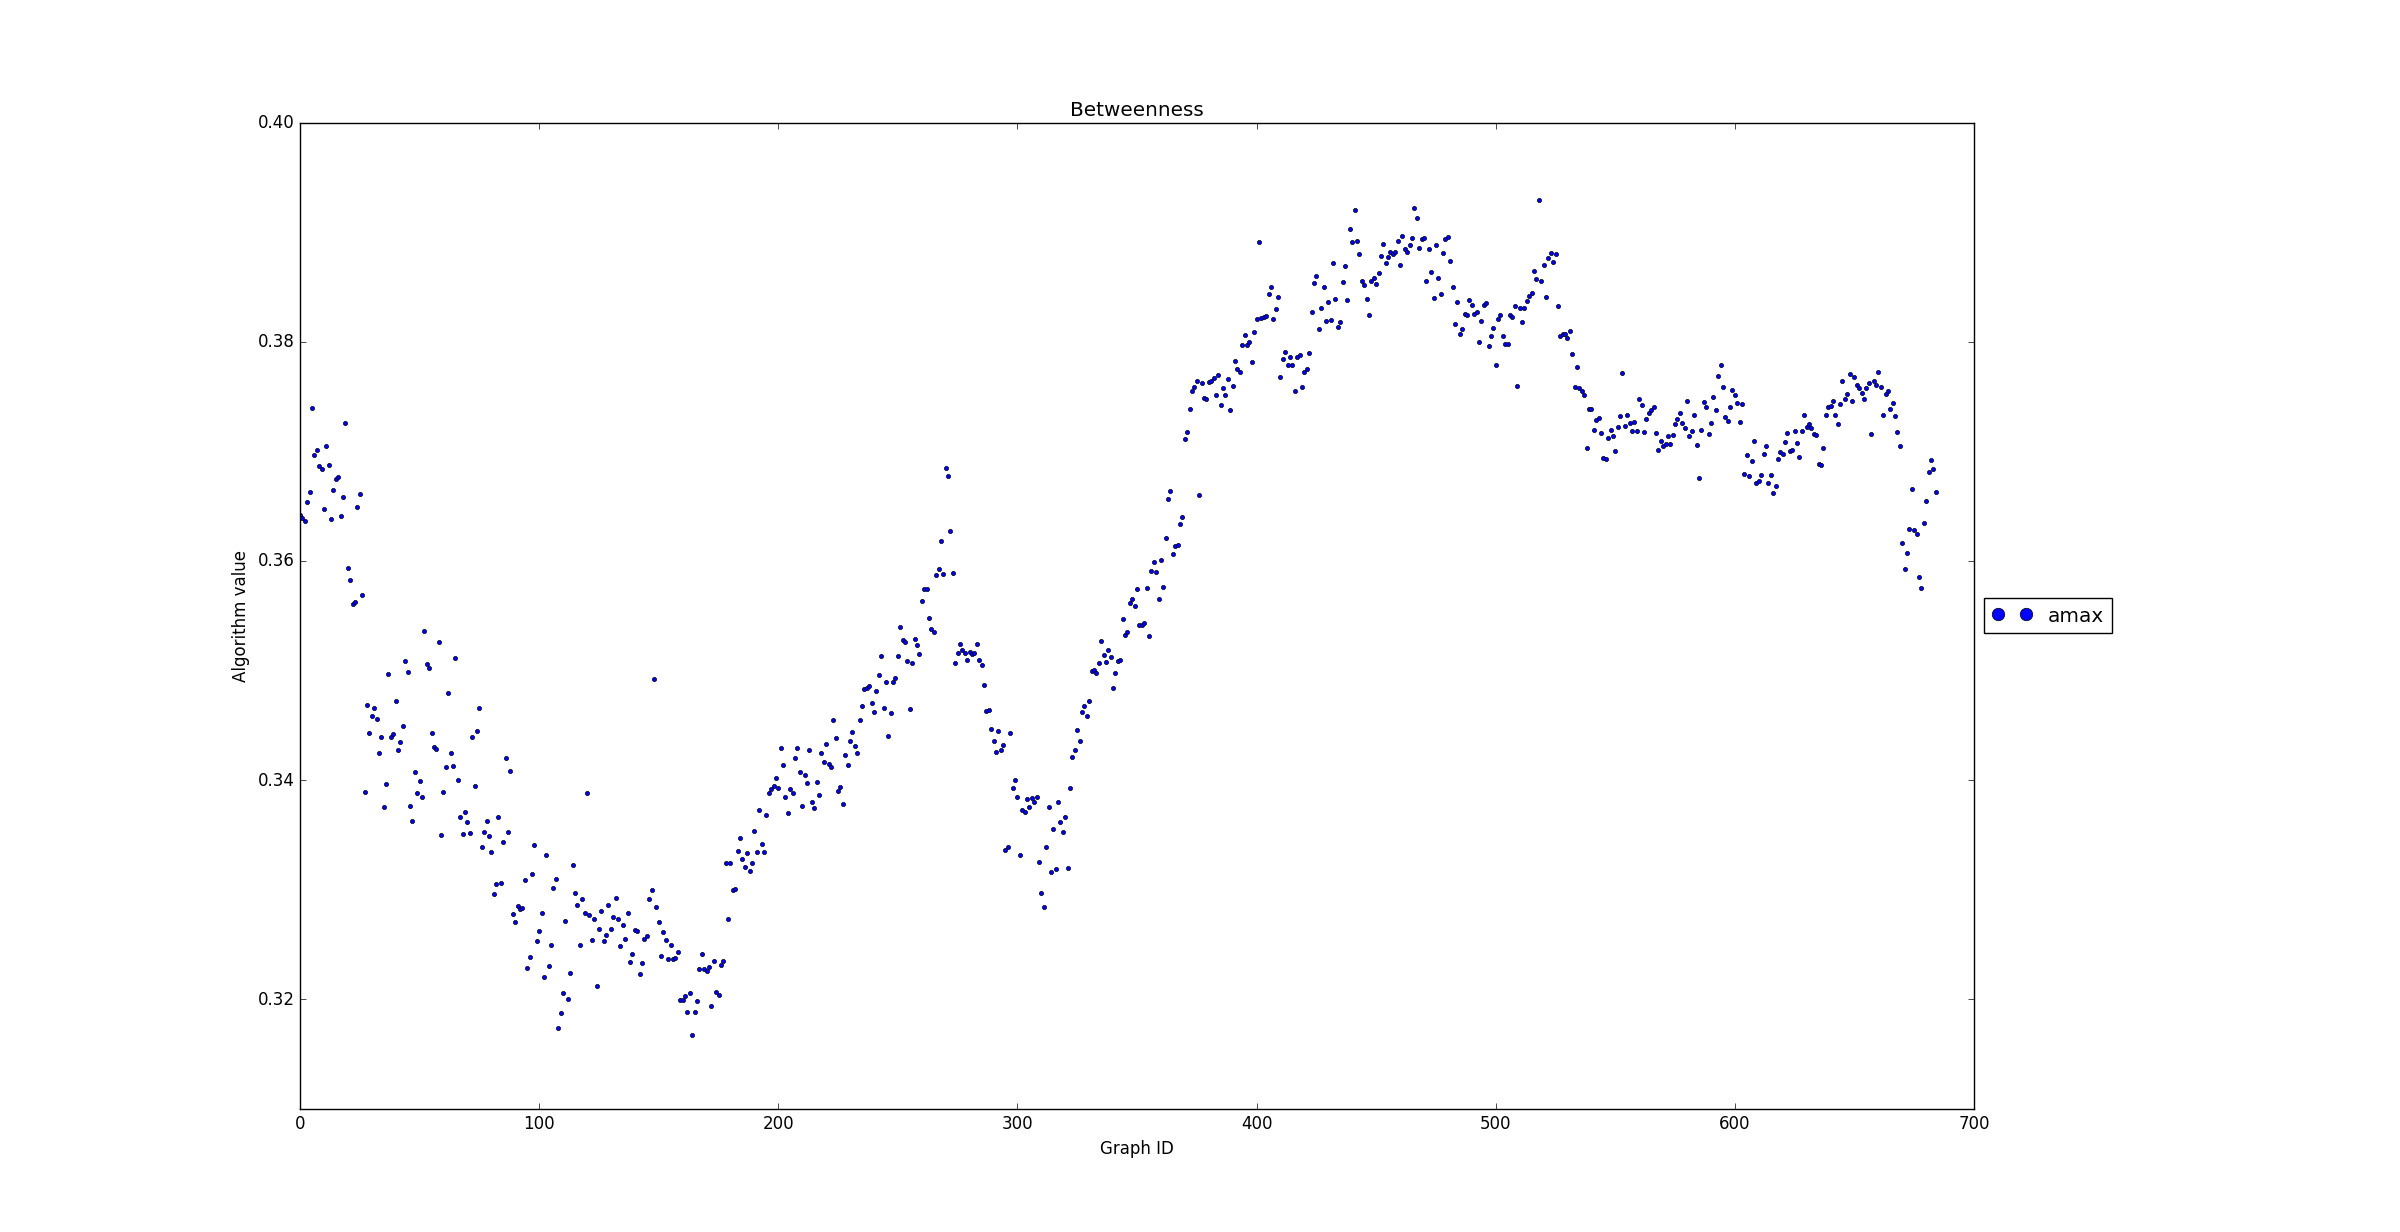
\includegraphics[width=\textwidth]{betweenness_max}
	\caption{Działanie Betweenness Centrality  na przykładowym grafie}
\end{figure}
\FloatBarrier\FloatBarrier
\subsubsection{Przykład}
\begin{figure}[h]
	\centering
	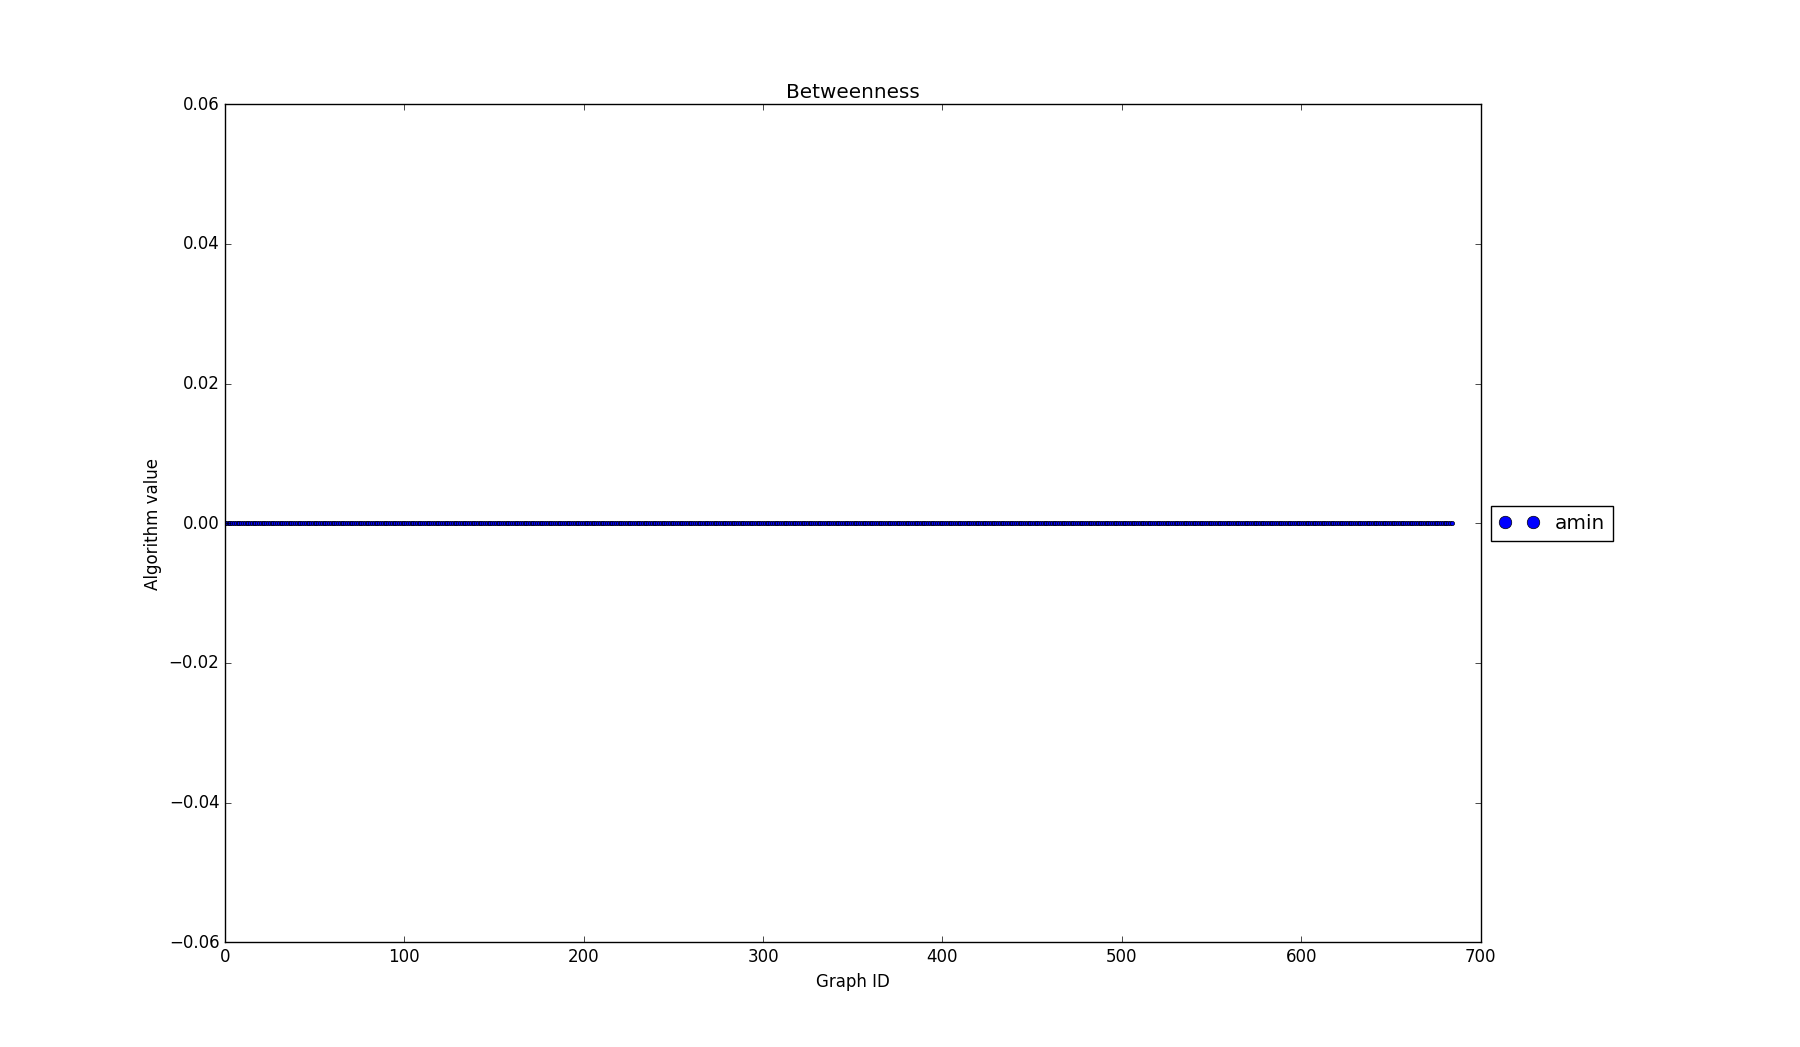
\includegraphics[width=\textwidth]{betweenness_min}
	\caption{Działanie Betweenness Centrality  na przykładowym grafie}
\end{figure}
\FloatBarrier\FloatBarrier
\subsubsection{Przykład}
\begin{figure}[h]
	\centering
	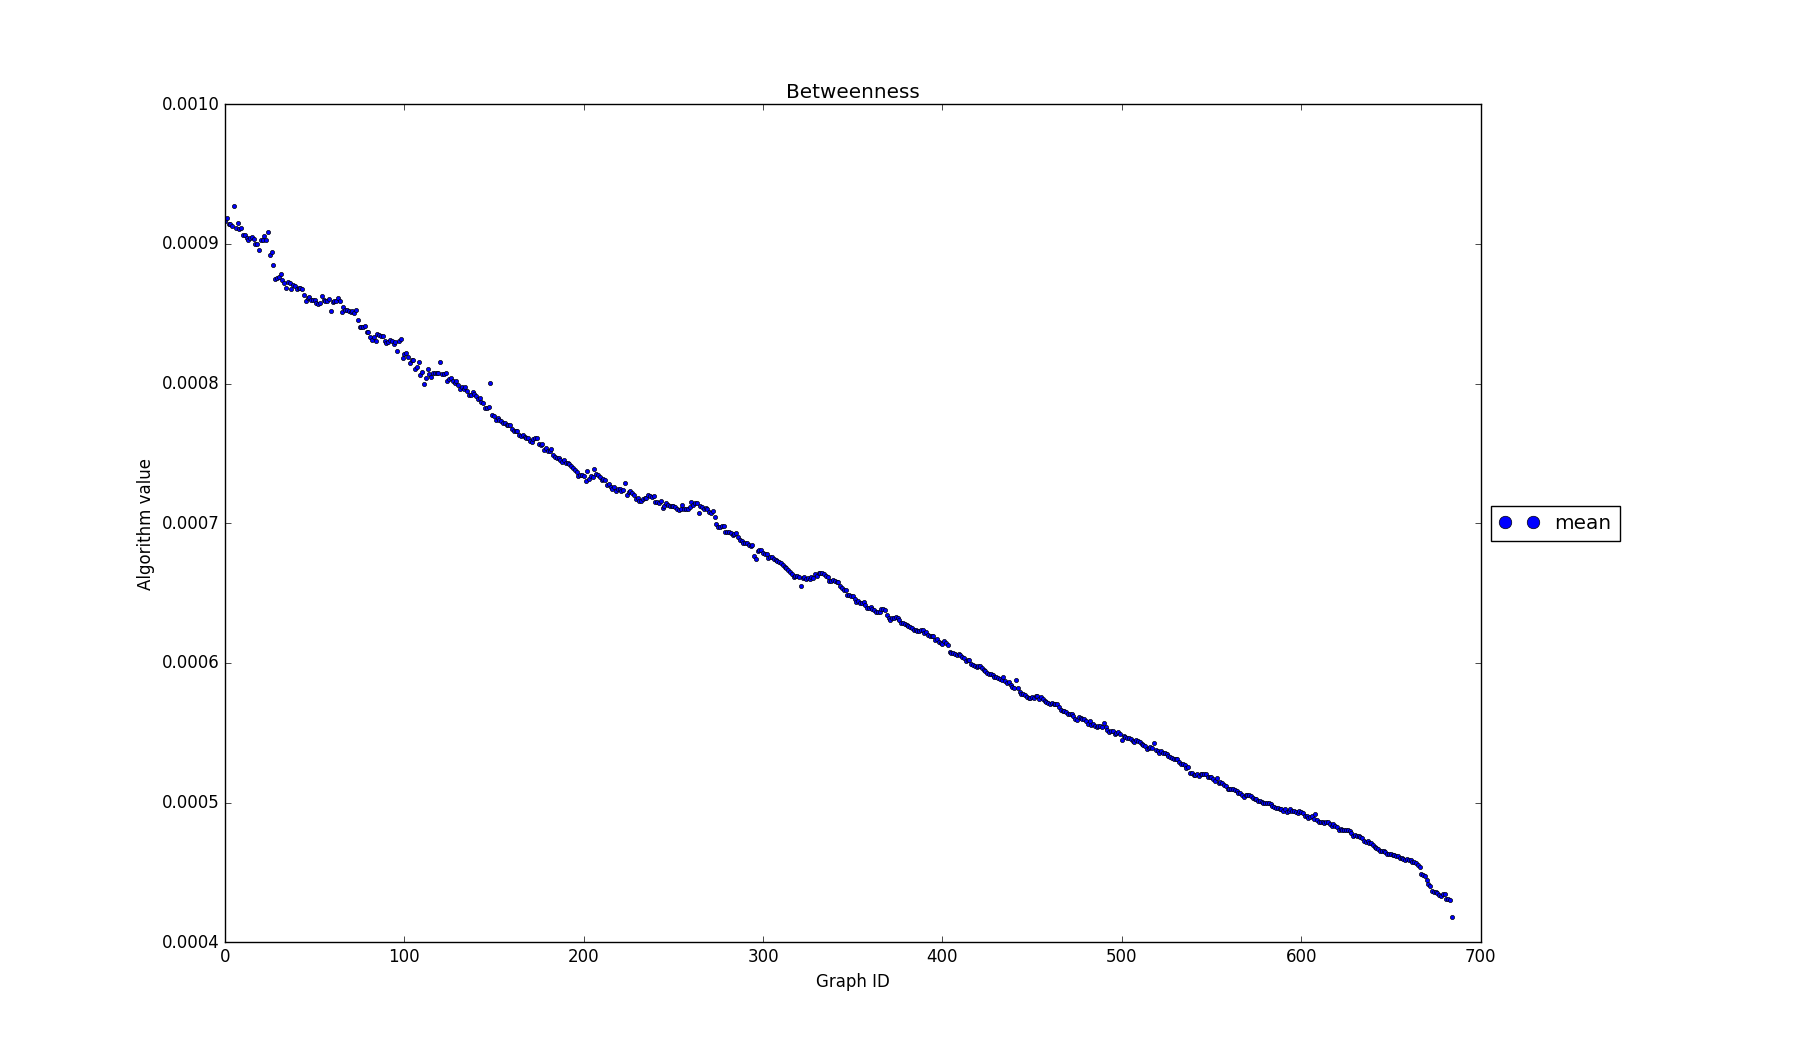
\includegraphics[width=\textwidth]{betweenness_mean}
	\caption{Działanie Betweenness Centrality  na przykładowym grafie}
\end{figure}
\FloatBarrier\FloatBarrier
\subsubsection{Przykład}
\begin{figure}[h]
	\centering
	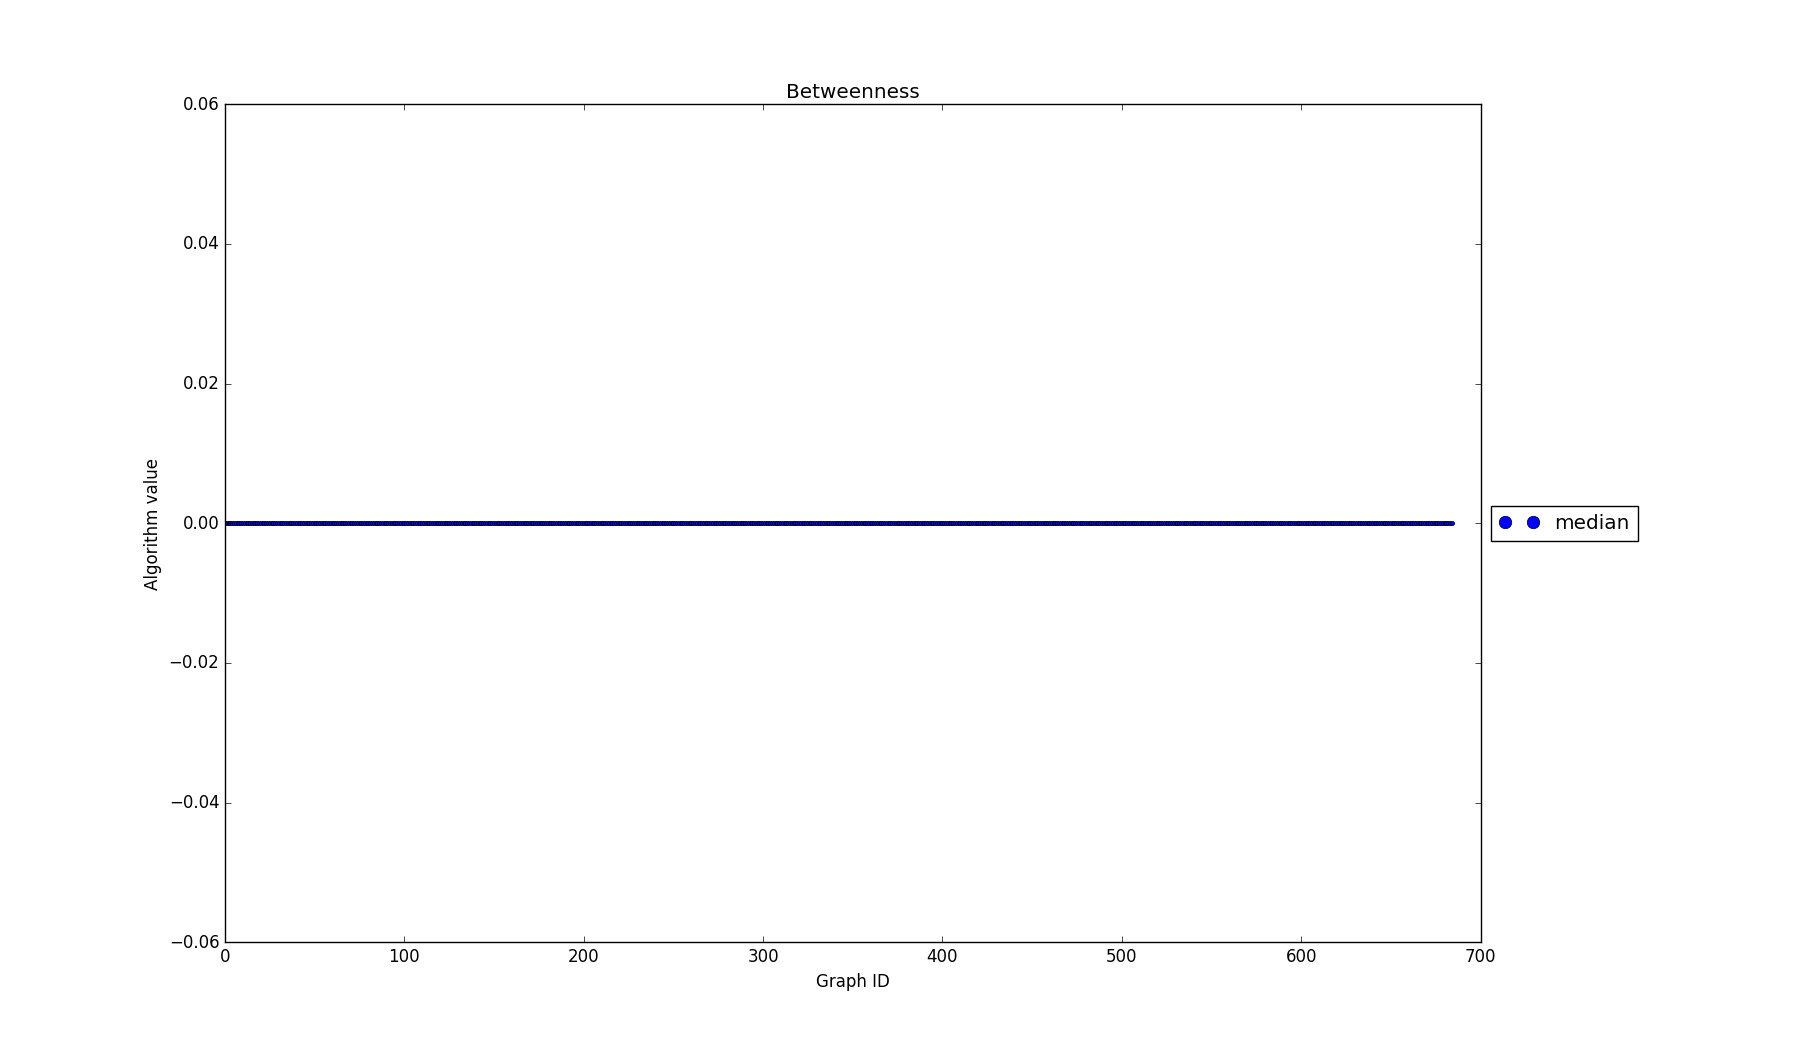
\includegraphics[width=\textwidth]{betweenness_median}
	\caption{Działanie Betweenness Centrality  na przykładowym grafie}
\end{figure}
\FloatBarrier
\section{Closeness}
\FloatBarrier
\begin{figure}[h]
	\centering
	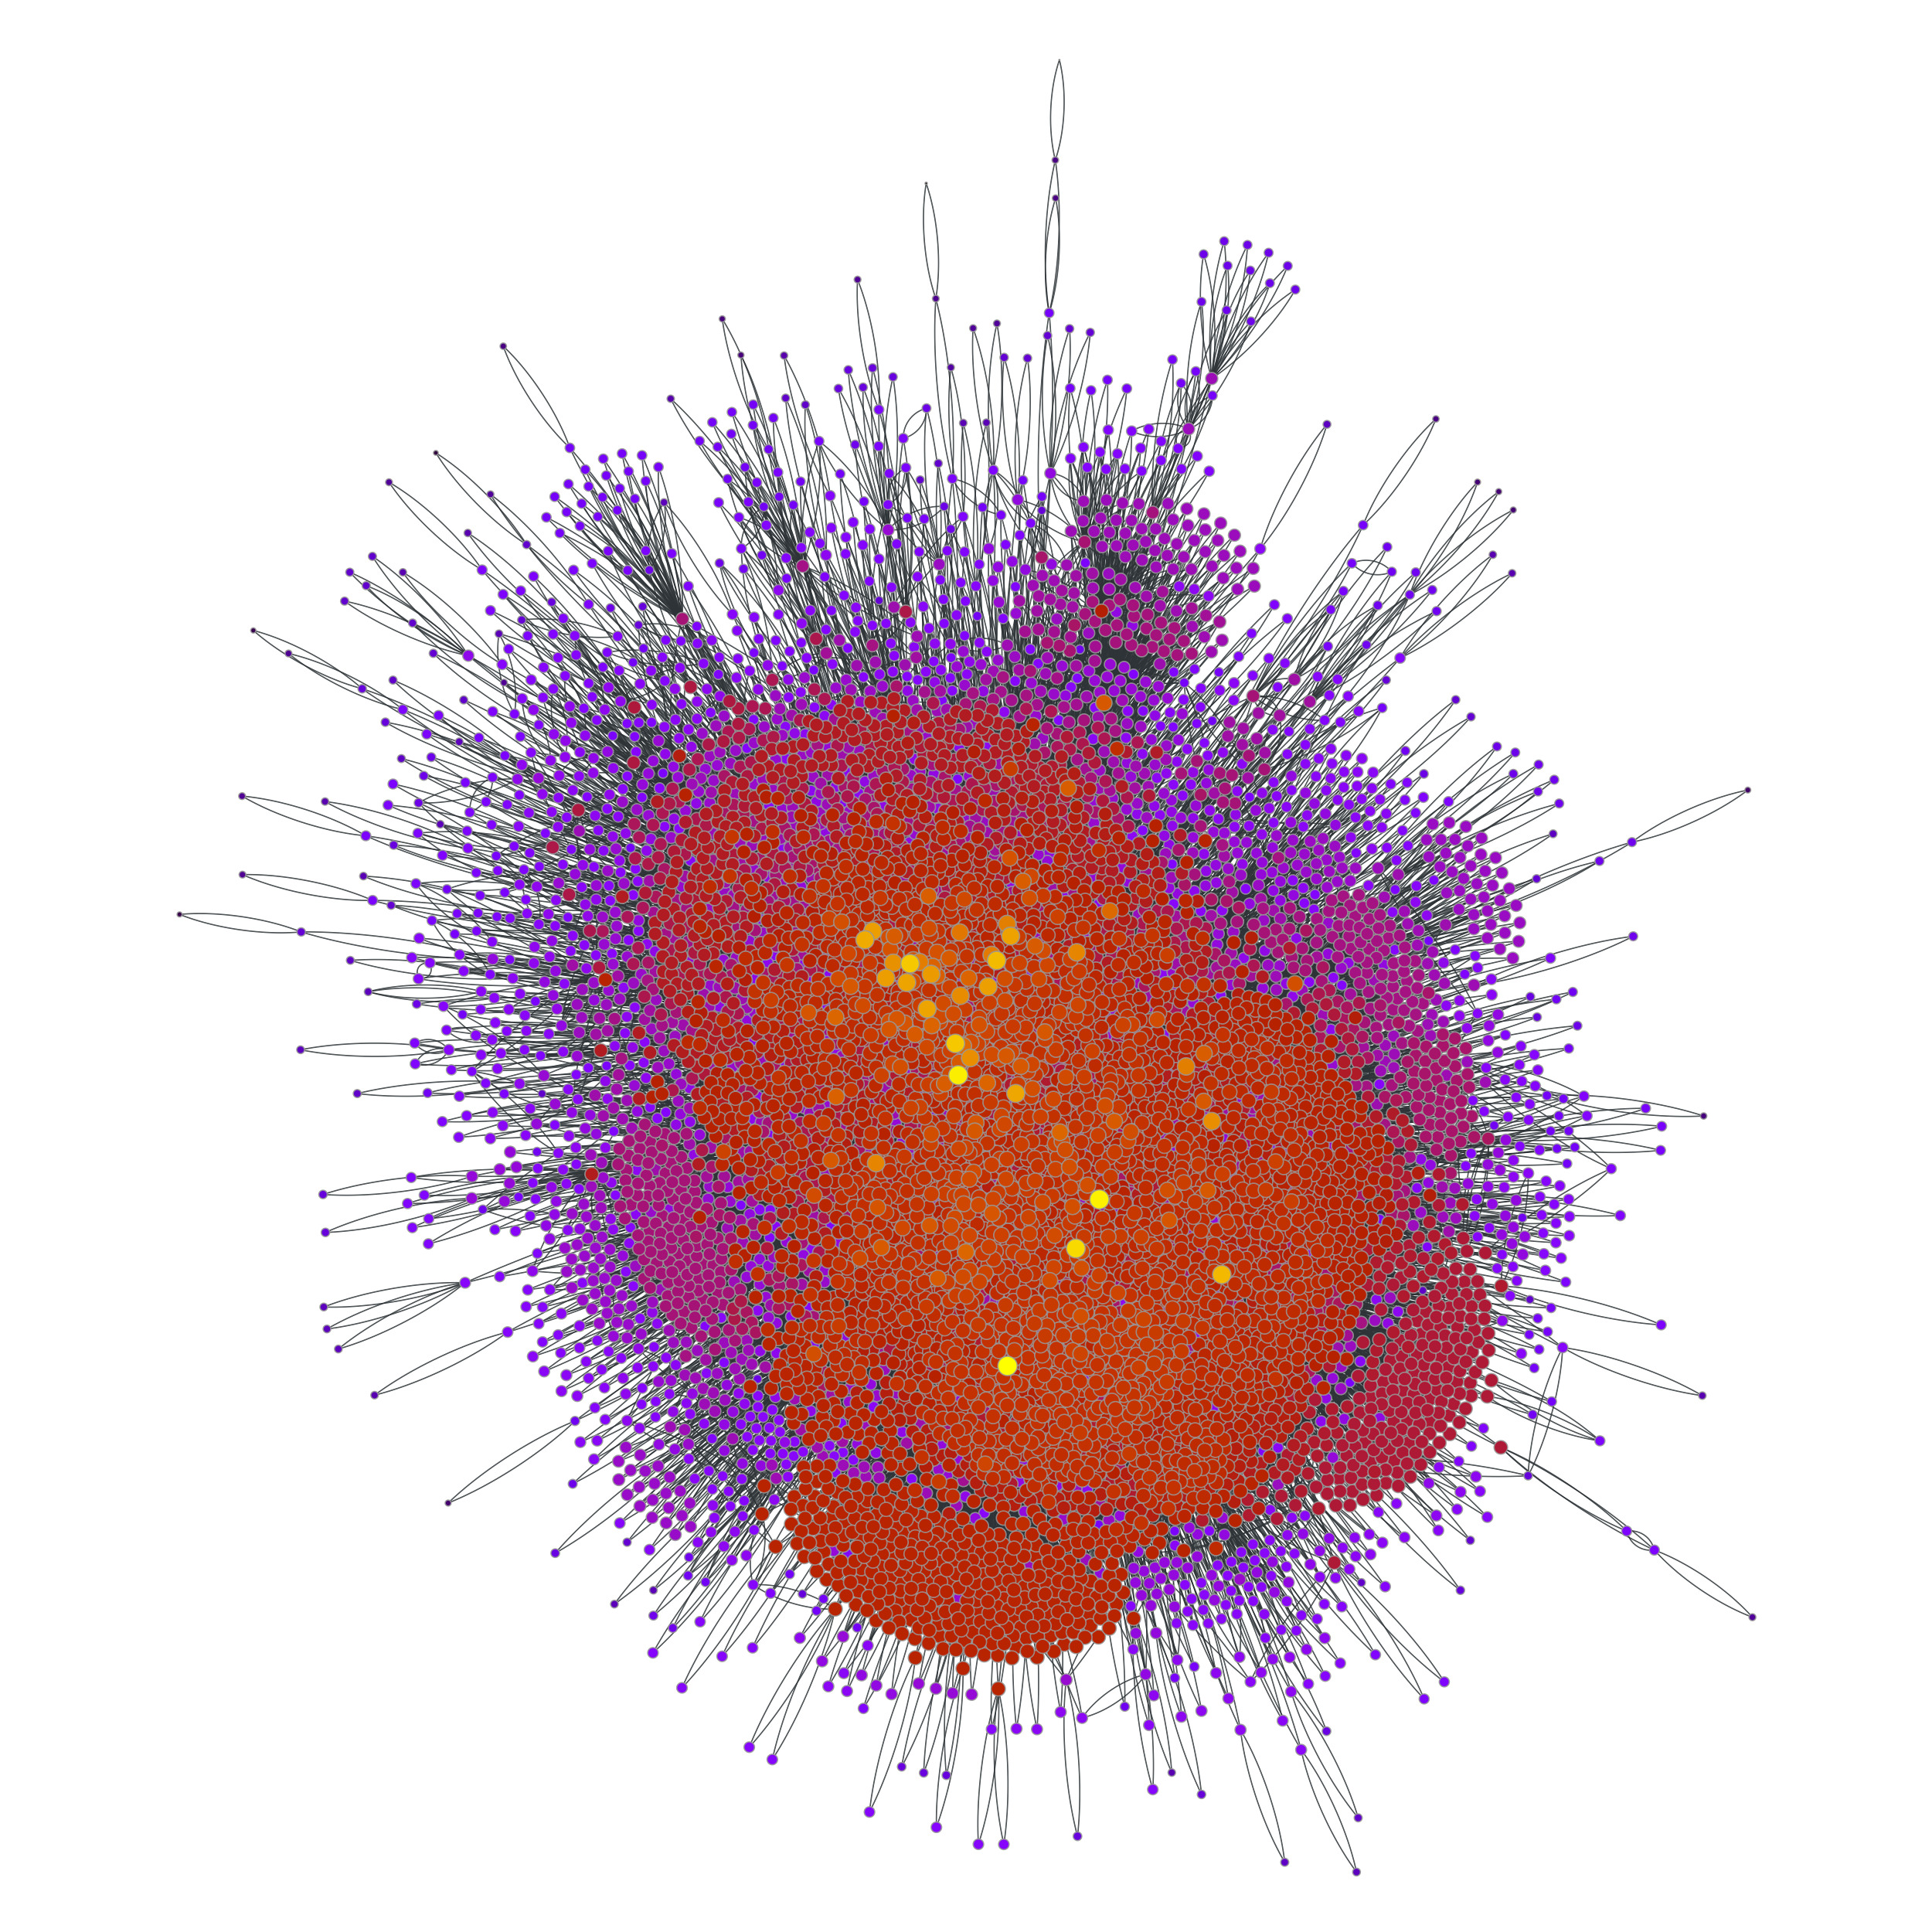
\includegraphics[width=\textwidth]{closeness_8k}
	\caption{Działanie algorytmu closeness na przykładowym grafie}
\end{figure}
\FloatBarrier
Powyżej przedstawione jest działanie algorytmu closeness na wybranym grafie. Kolor oraz wielkość wierzchołka zależy od wyniku algorytmu. Duże i jasne wierzchołki są wierzchołkami, z których najłatwiej dostać się do innych - wymagają średnio najmniej przeskoków by dostać się do innego wierzchołka. Przekłada się to bezpośrednio na to, że dany wierzchołek - fragment sieci może być często wybierany jako pośrednik.
\FloatBarrier
\begin{figure}[h]
	\centering
	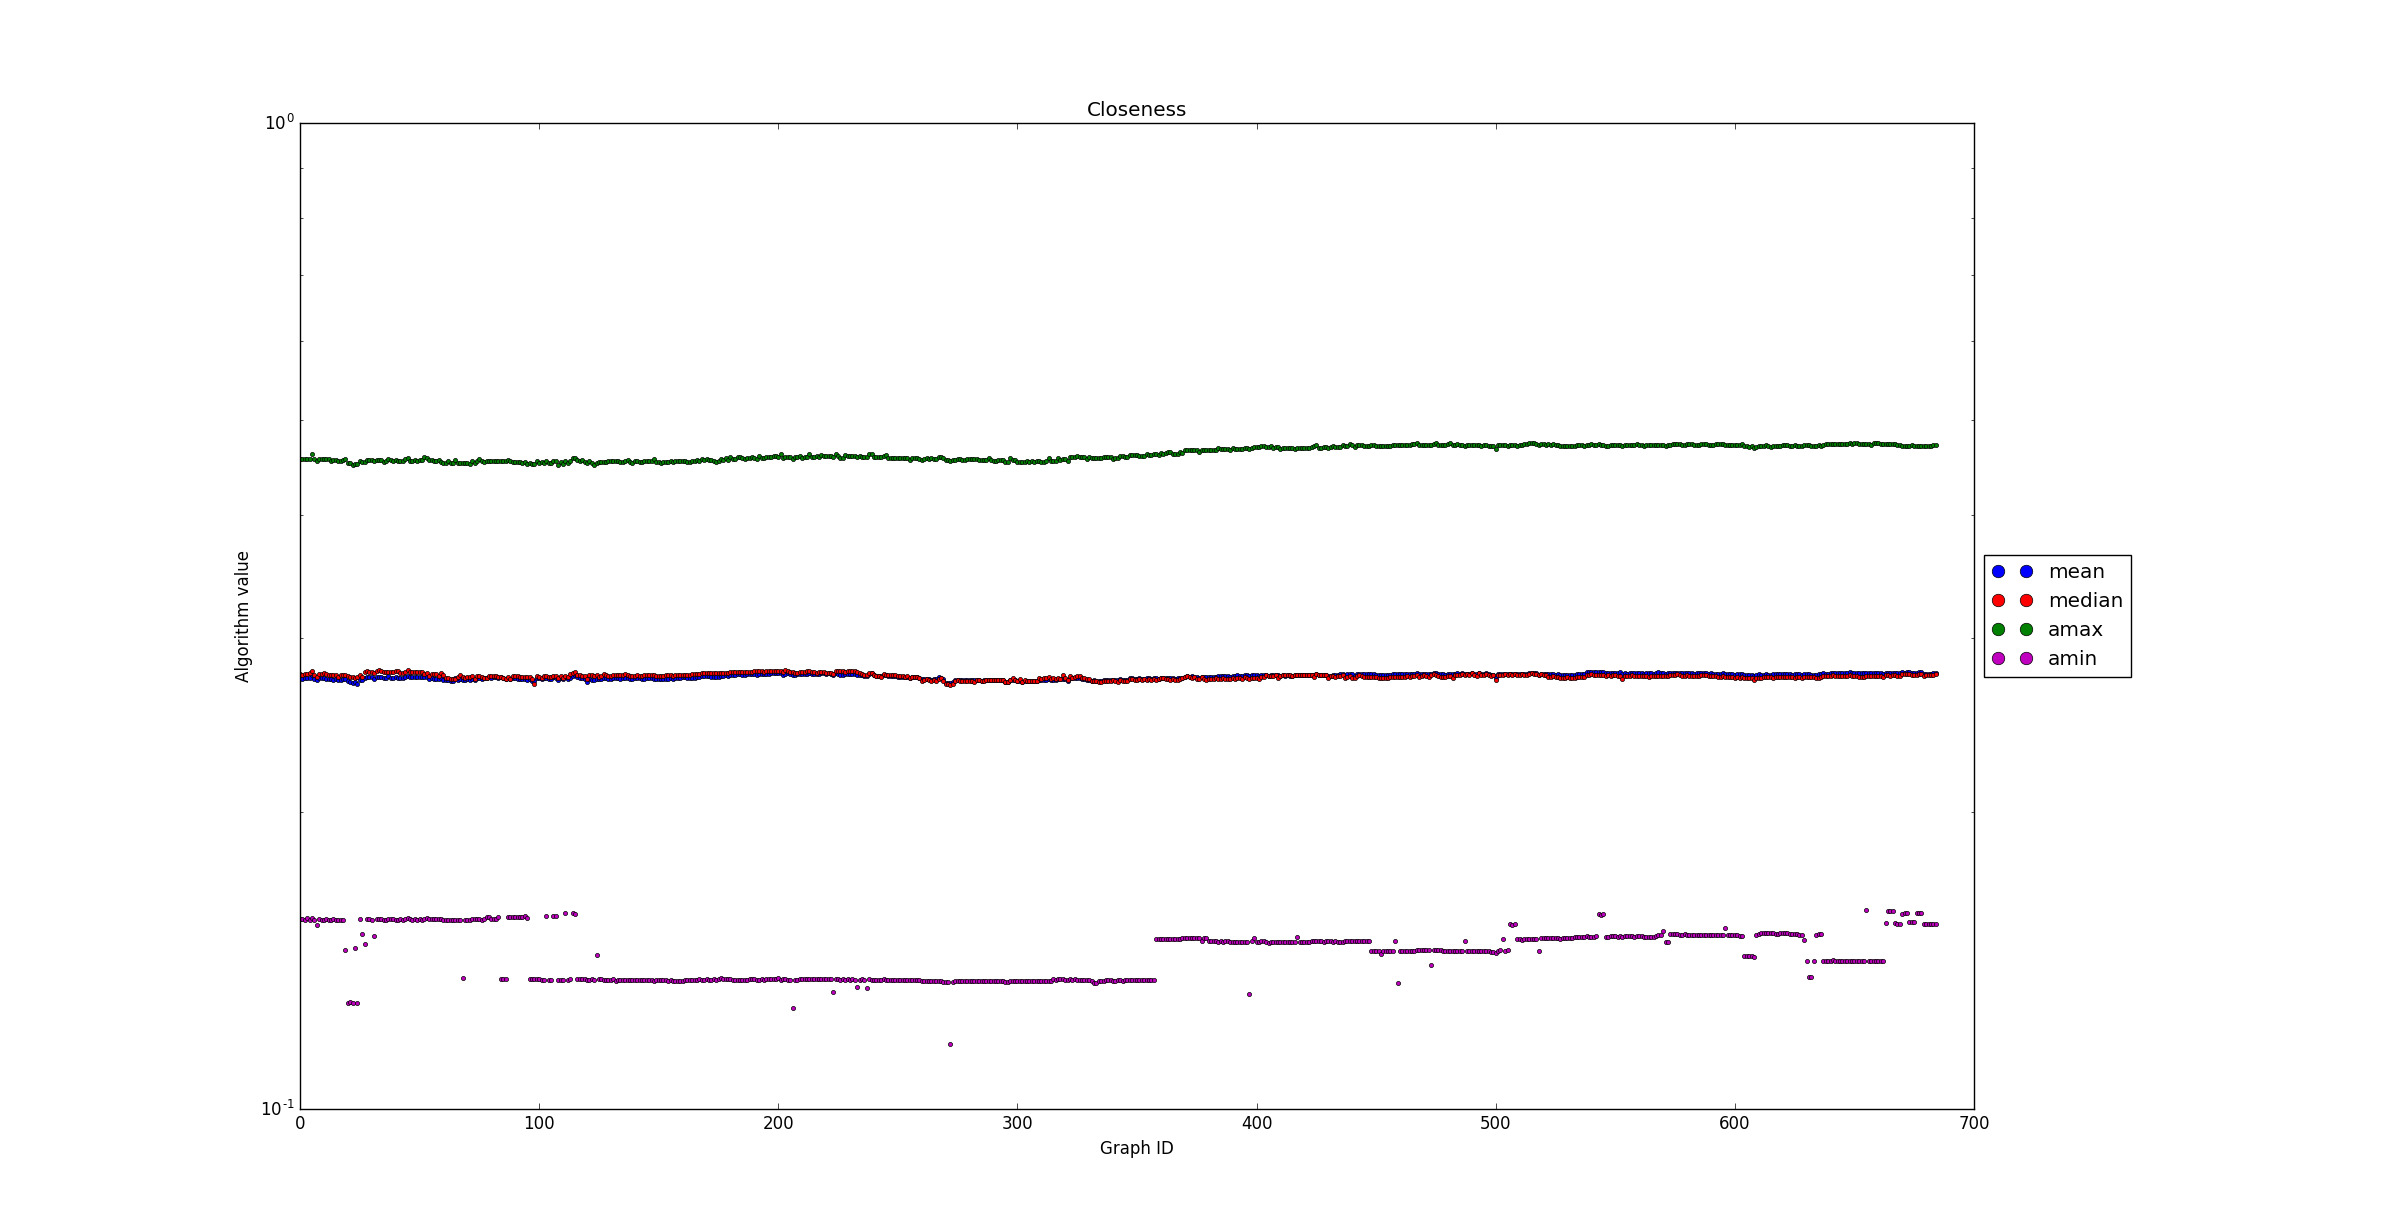
\includegraphics[width=\textwidth]{closeness}
	\caption{Wyniki algorytmu closeness}
\end{figure}
\FloatBarrier\FloatBarrier
\begin{figure}[h]
	\centering
	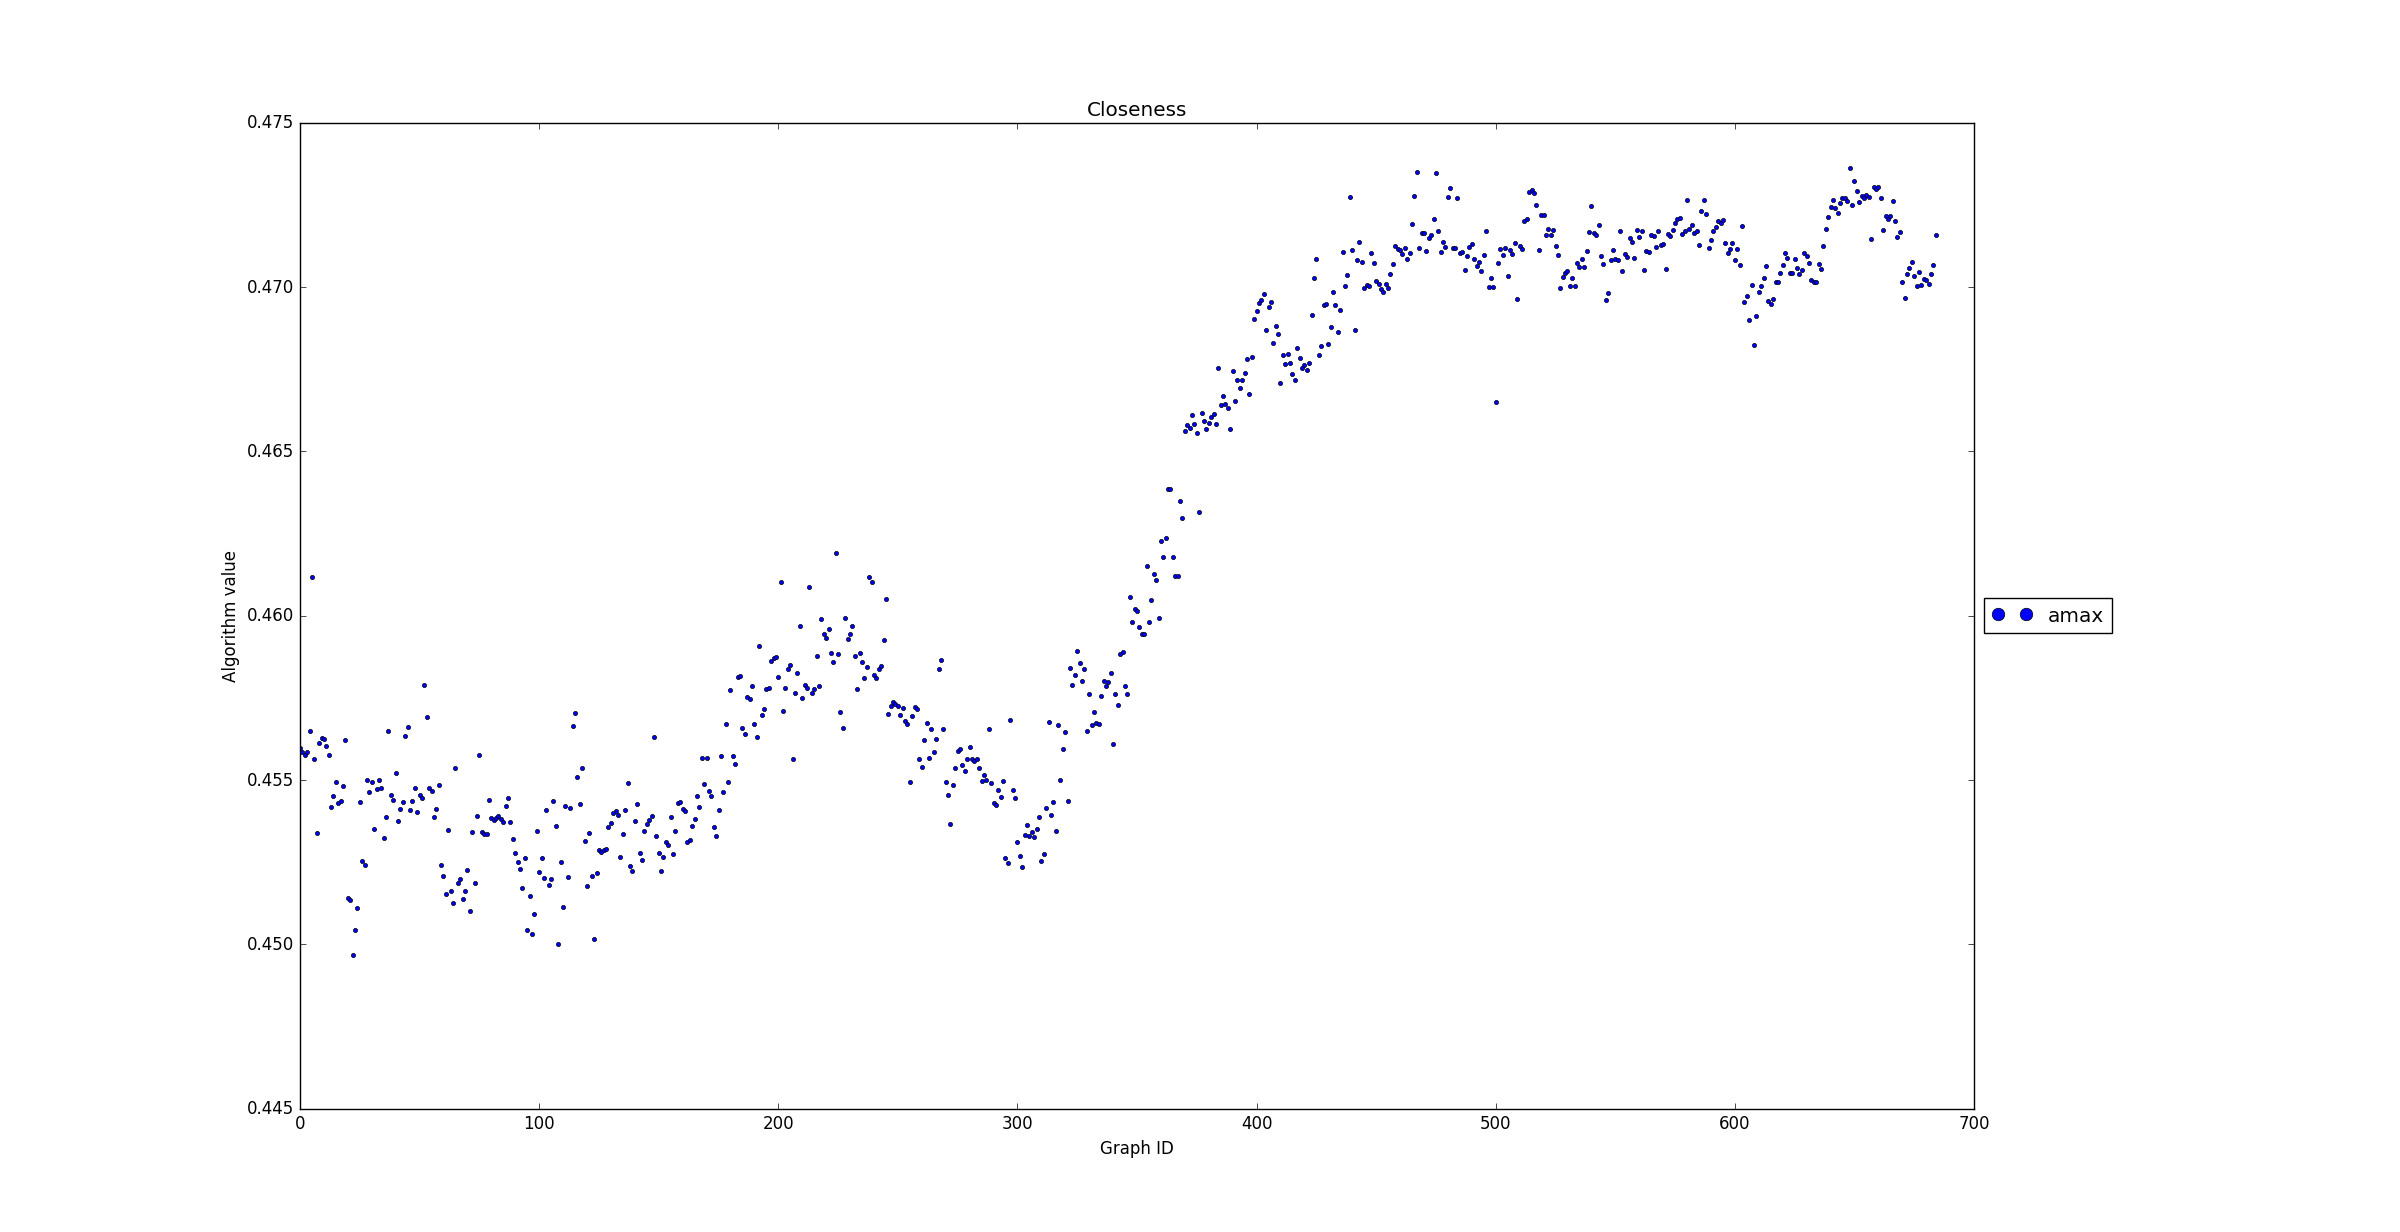
\includegraphics[width=\textwidth]{closeness_max}
	\caption{Maksymalne wartości closeness}
\end{figure}
\FloatBarrier\FloatBarrier
\begin{figure}[h]
	\centering
	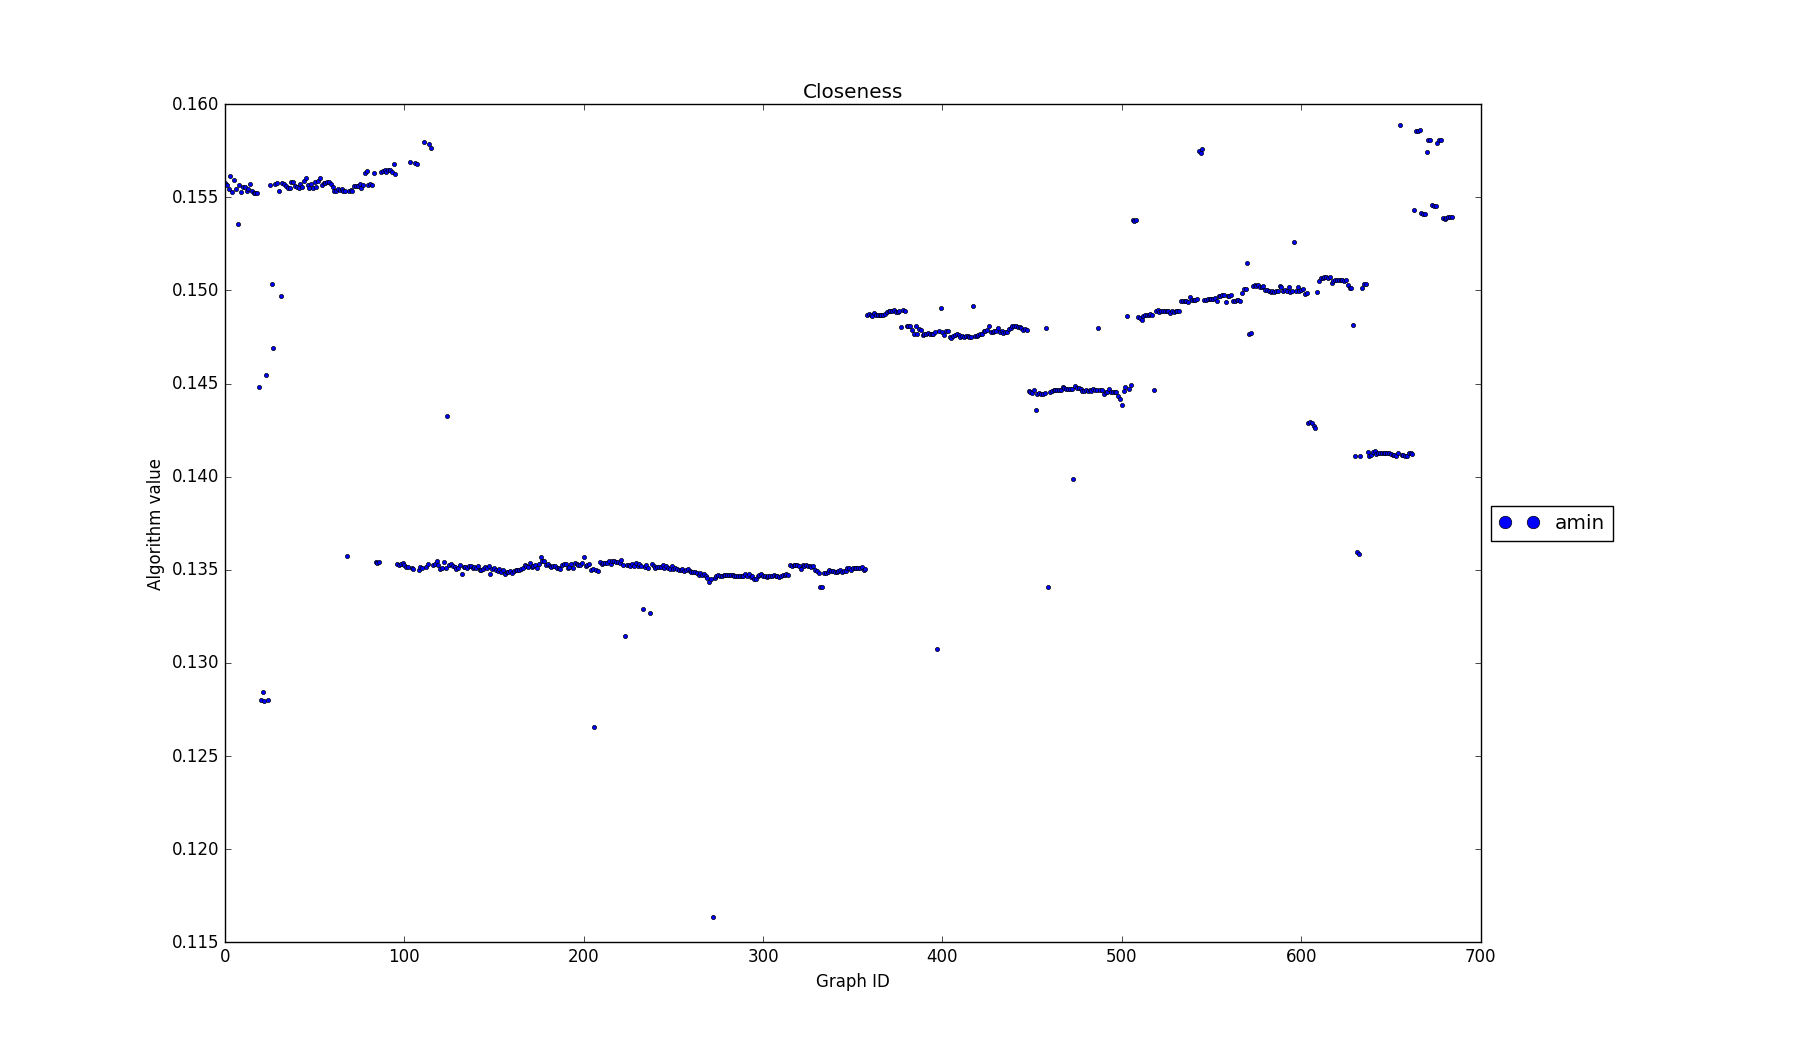
\includegraphics[width=\textwidth]{closeness_min}
	\caption{Minimalne wartości closeness}
\end{figure}
\FloatBarrier\FloatBarrier
\begin{figure}[h]
	\centering
	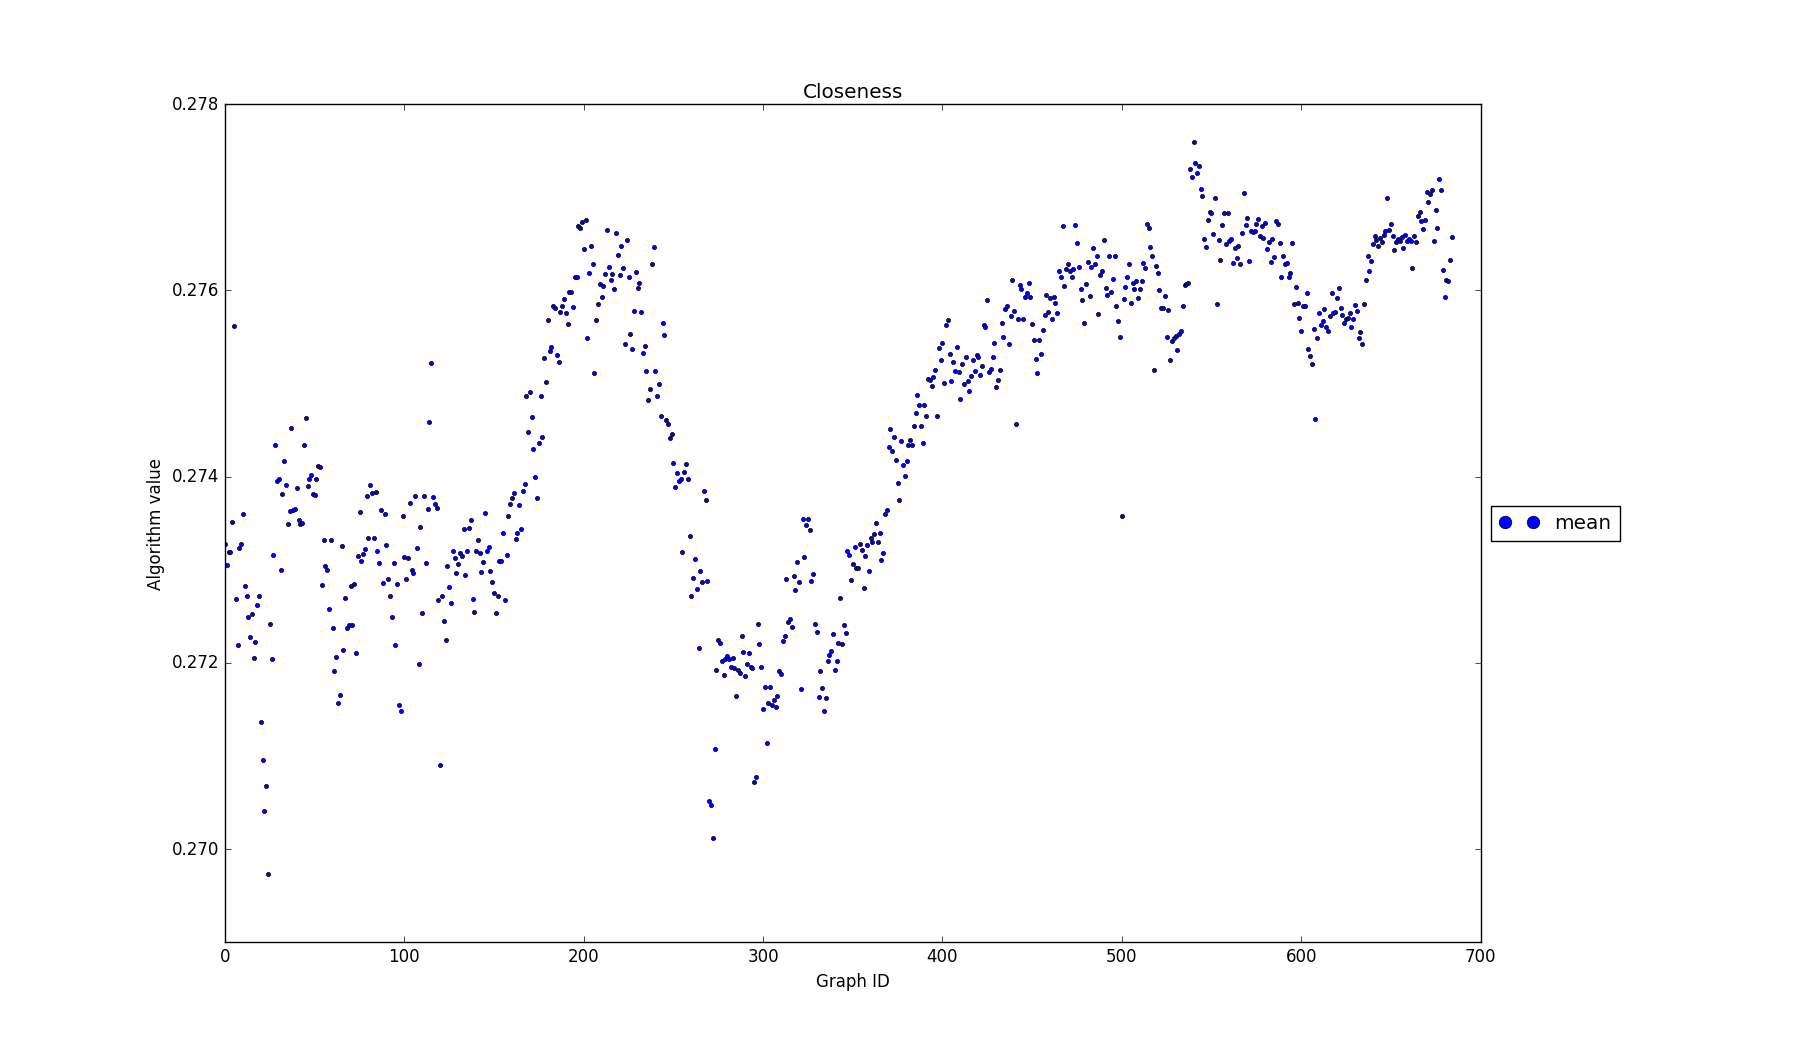
\includegraphics[width=\textwidth]{closeness_mean}
	\caption{Średnie wartości closeness}
\end{figure}
\FloatBarrier\FloatBarrier
\begin{figure}[h]
	\centering
	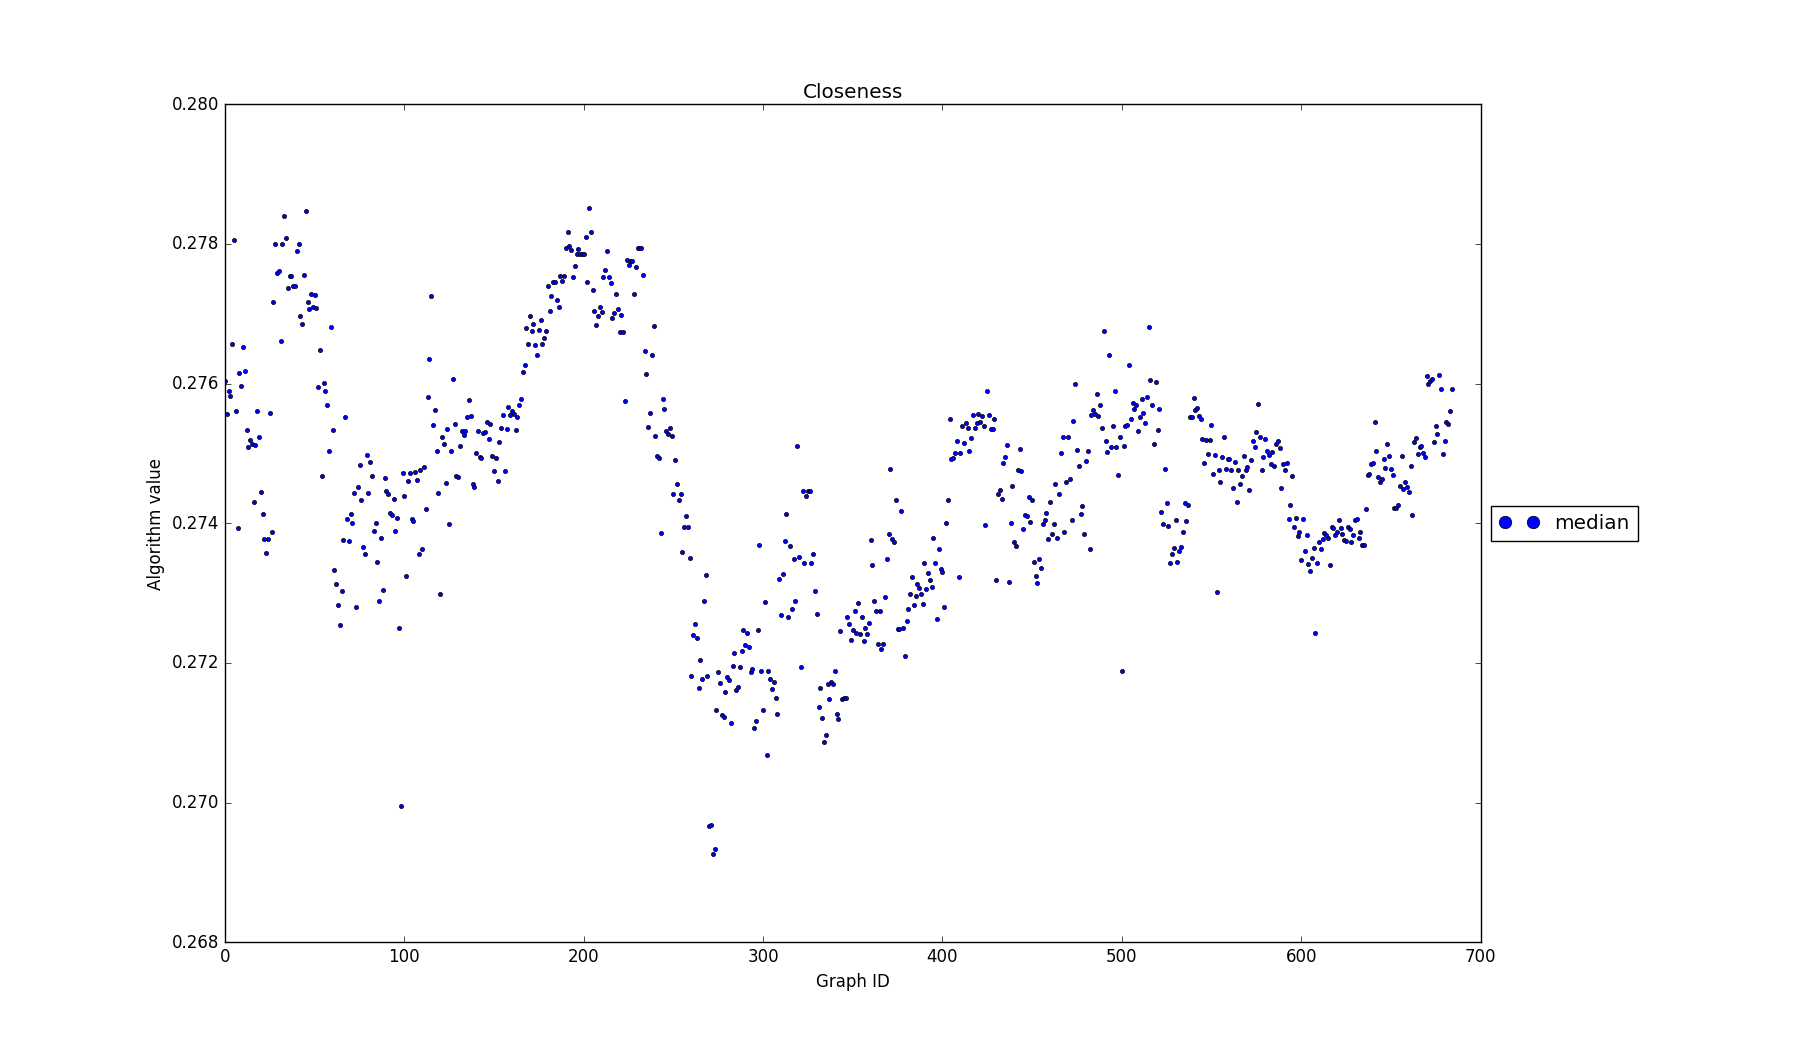
\includegraphics[width=\textwidth]{closeness_median}
	\caption{Mediana wartości closeness}
\end{figure}
\FloatBarrier
\newpage
\section{Pagerank}
\FloatBarrier\FloatBarrier
\begin{figure}[h]
	\centering
	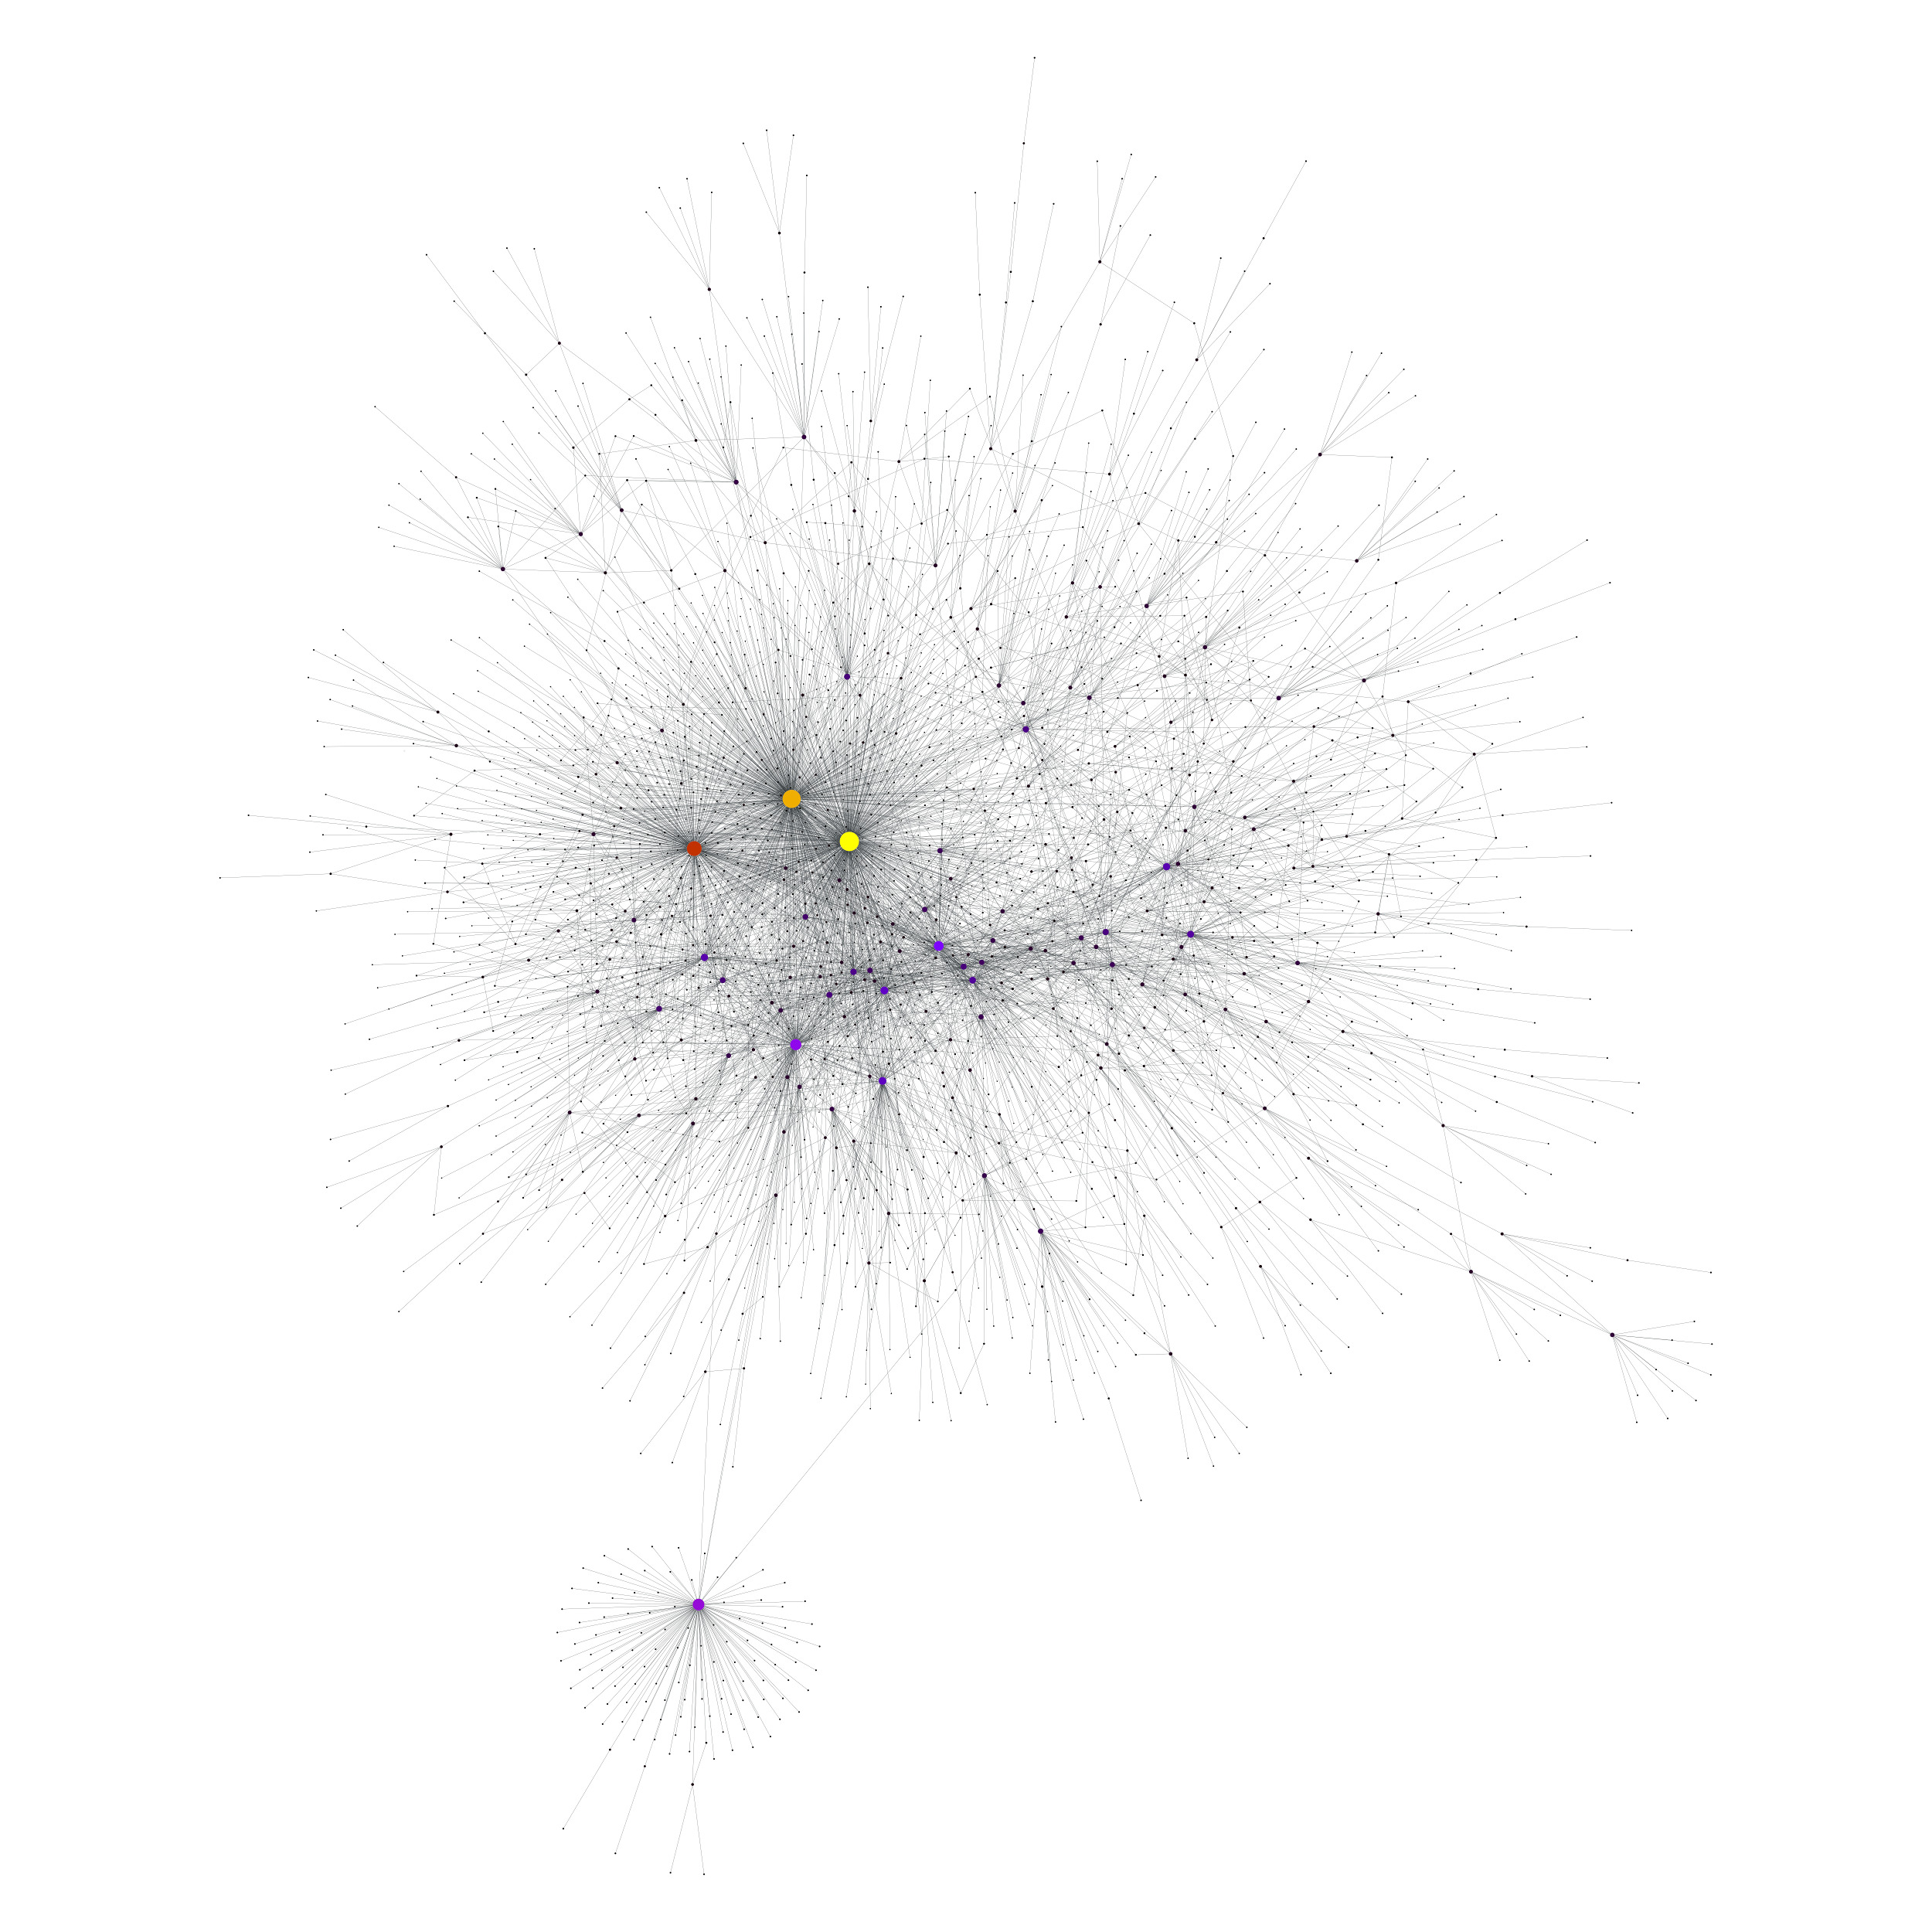
\includegraphics[width=\textwidth]{pagerank_8k}
	\caption{Działanie algorytmu pagerank na przykładowym grafie}
\end{figure}
\FloatBarrier
\begin{figure}[h]
	\centering
	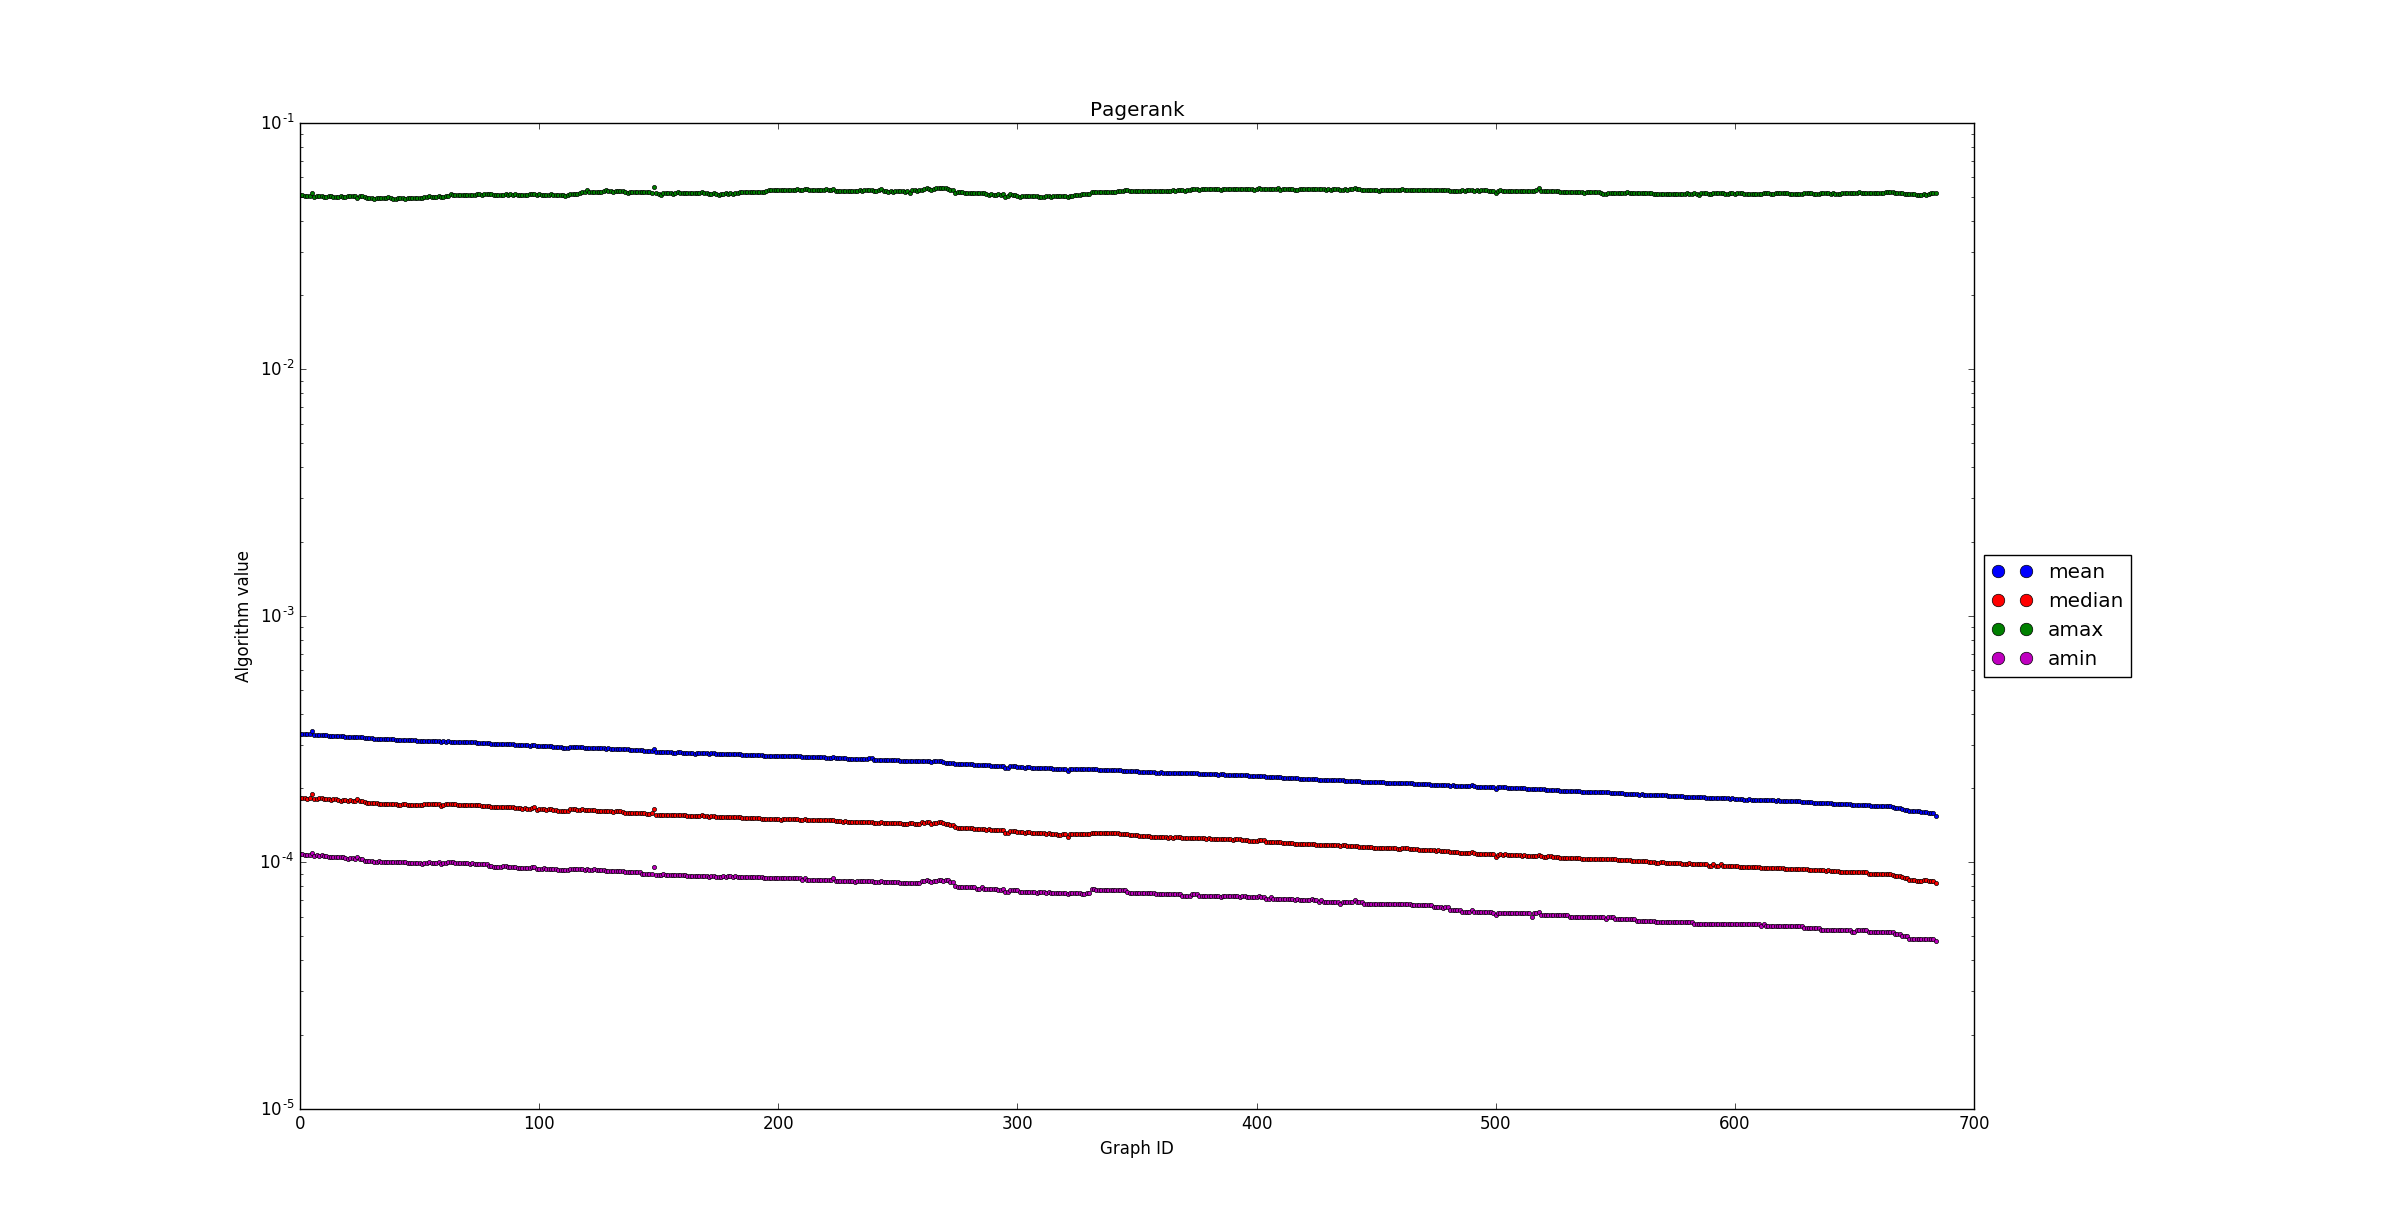
\includegraphics[width=\textwidth]{pagerank}
	\caption{Wyniki algorytmu pagerank}
\end{figure}
\FloatBarrier\FloatBarrier
\begin{figure}[h]
	\centering
	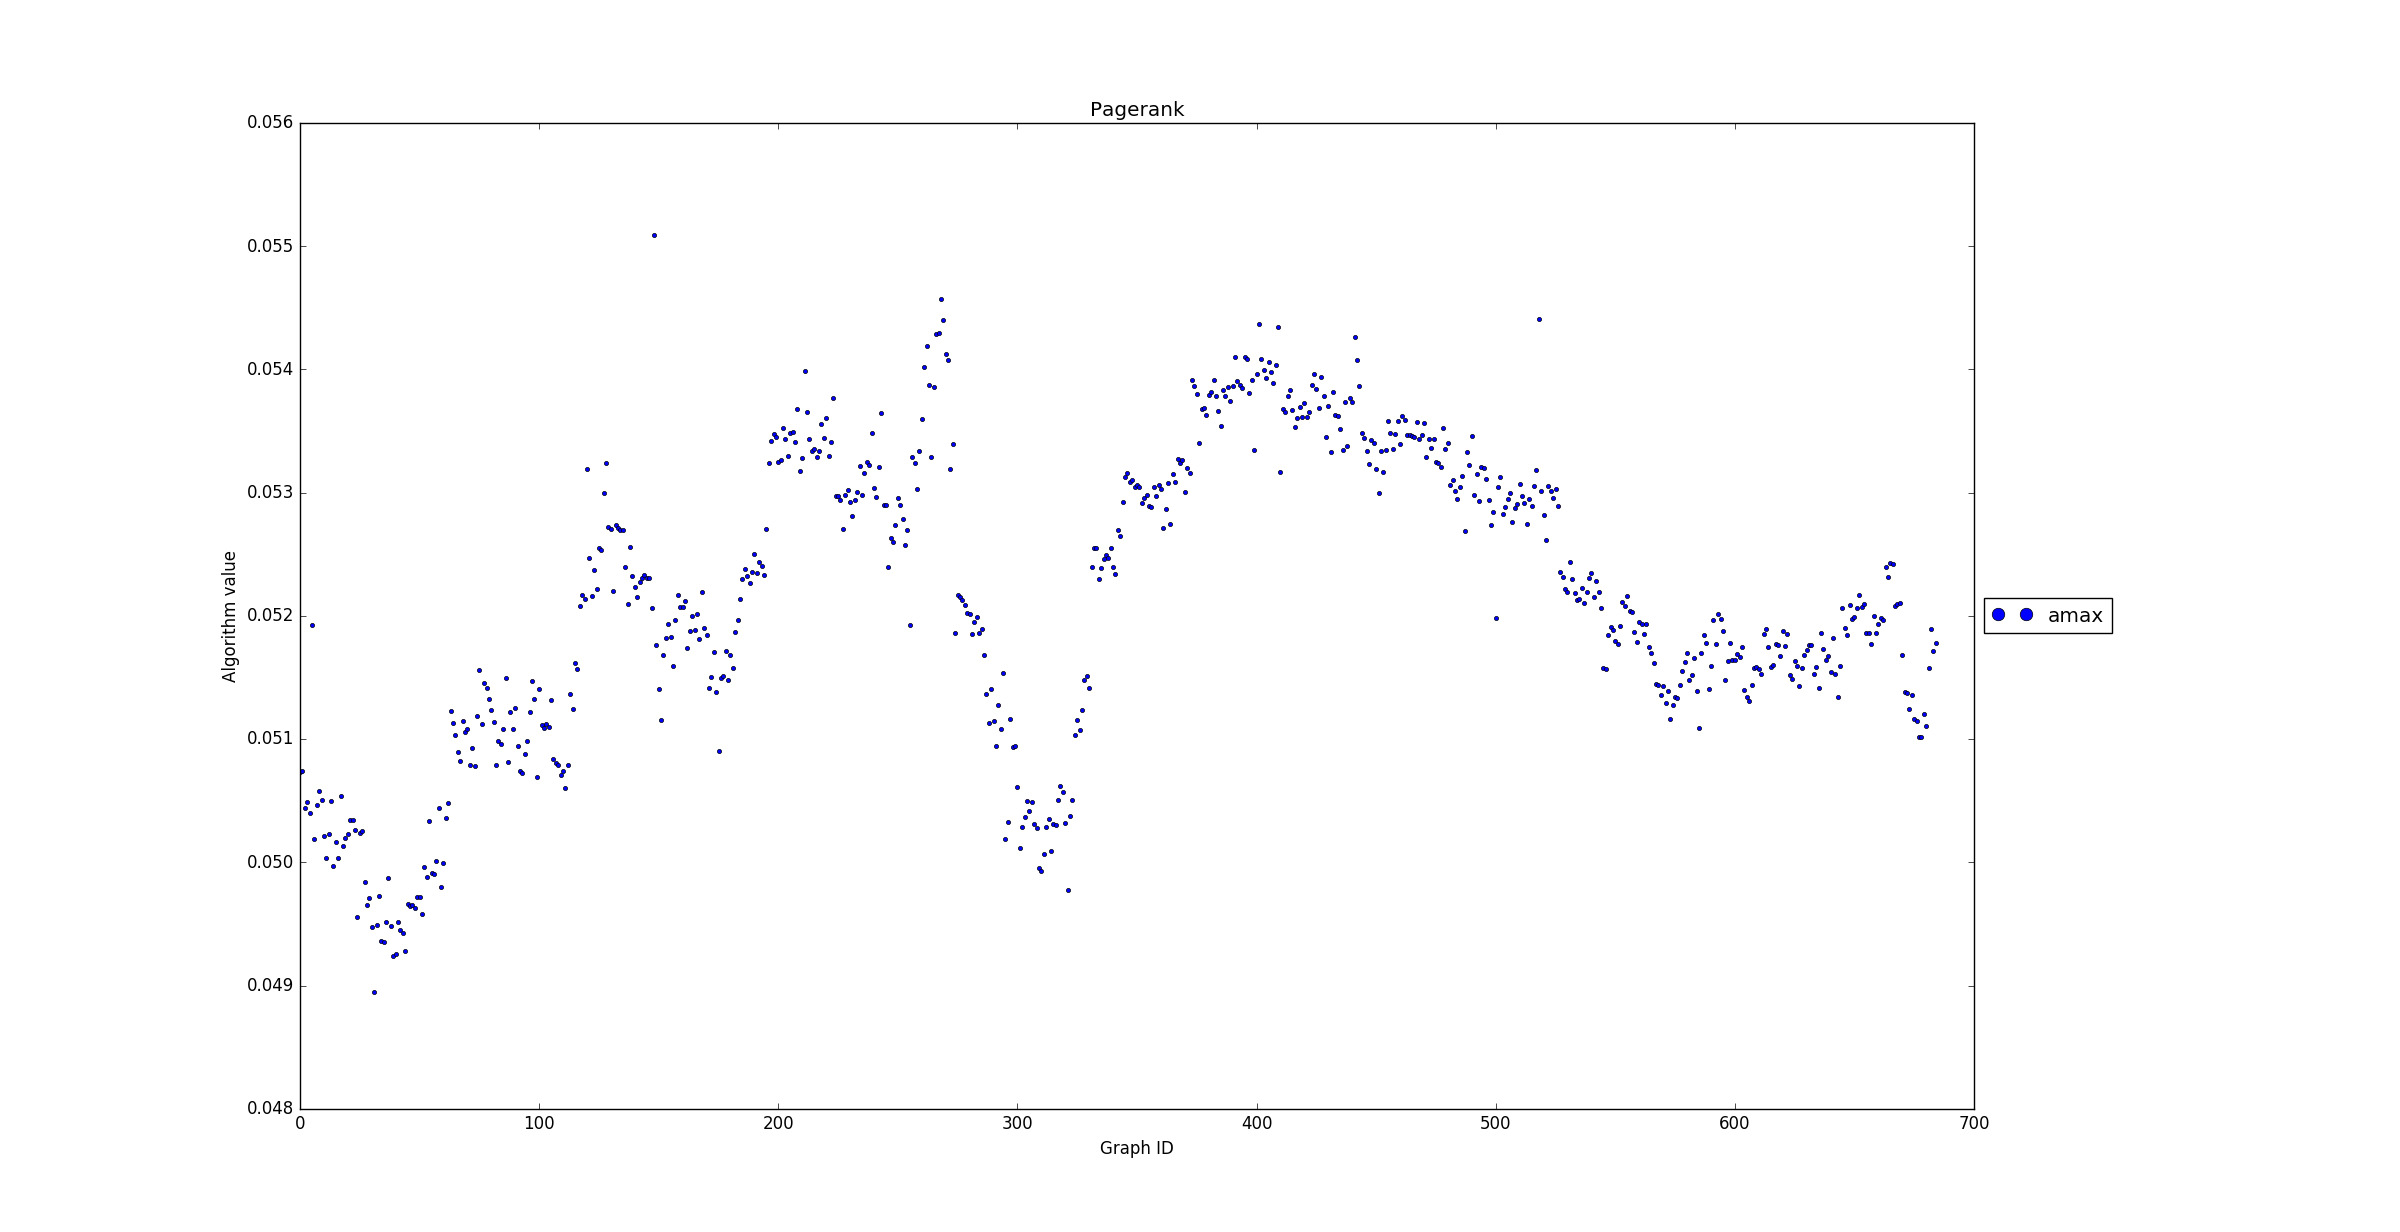
\includegraphics[width=\textwidth]{pagerank_max}
	\caption{Maksymalne wartości pagerank}
\end{figure}
\FloatBarrier\FloatBarrier
\begin{figure}[h]
	\centering
	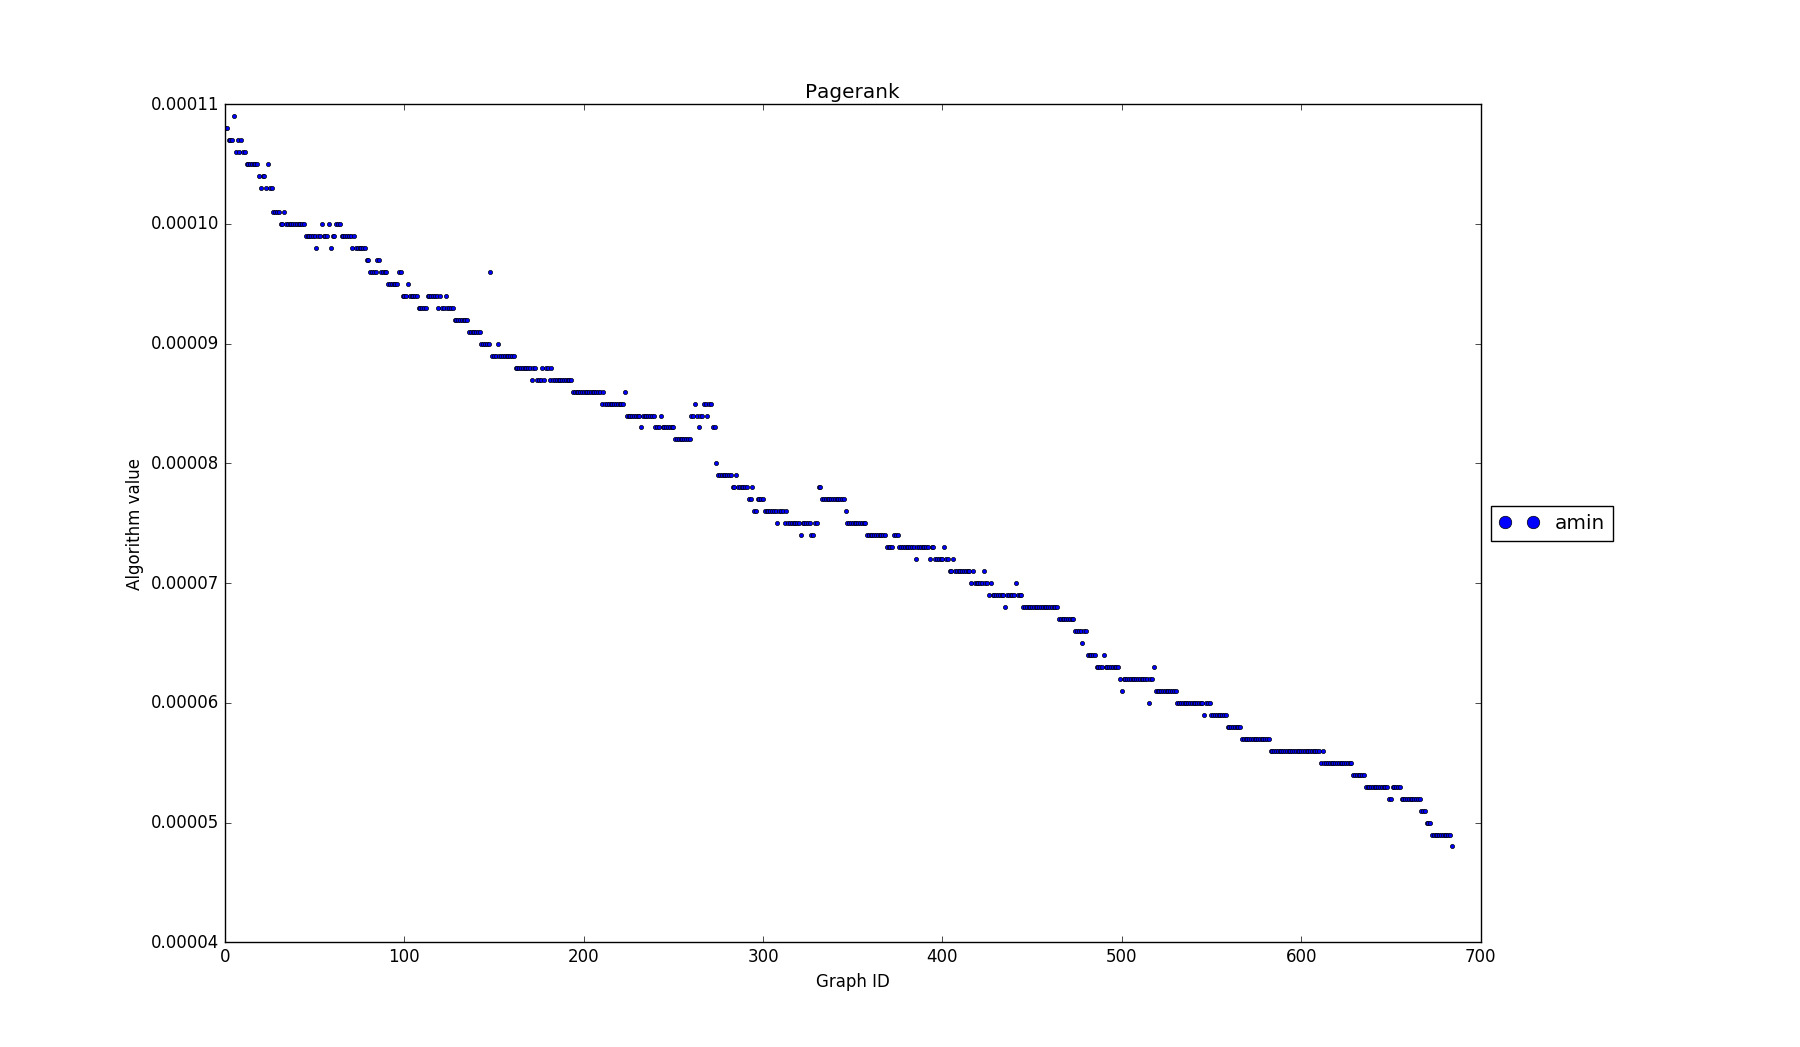
\includegraphics[width=\textwidth]{pagerank_min}
	\caption{Minimalne wartości pagerank}
\end{figure}
\FloatBarrier\FloatBarrier
\begin{figure}[h]
	\centering
	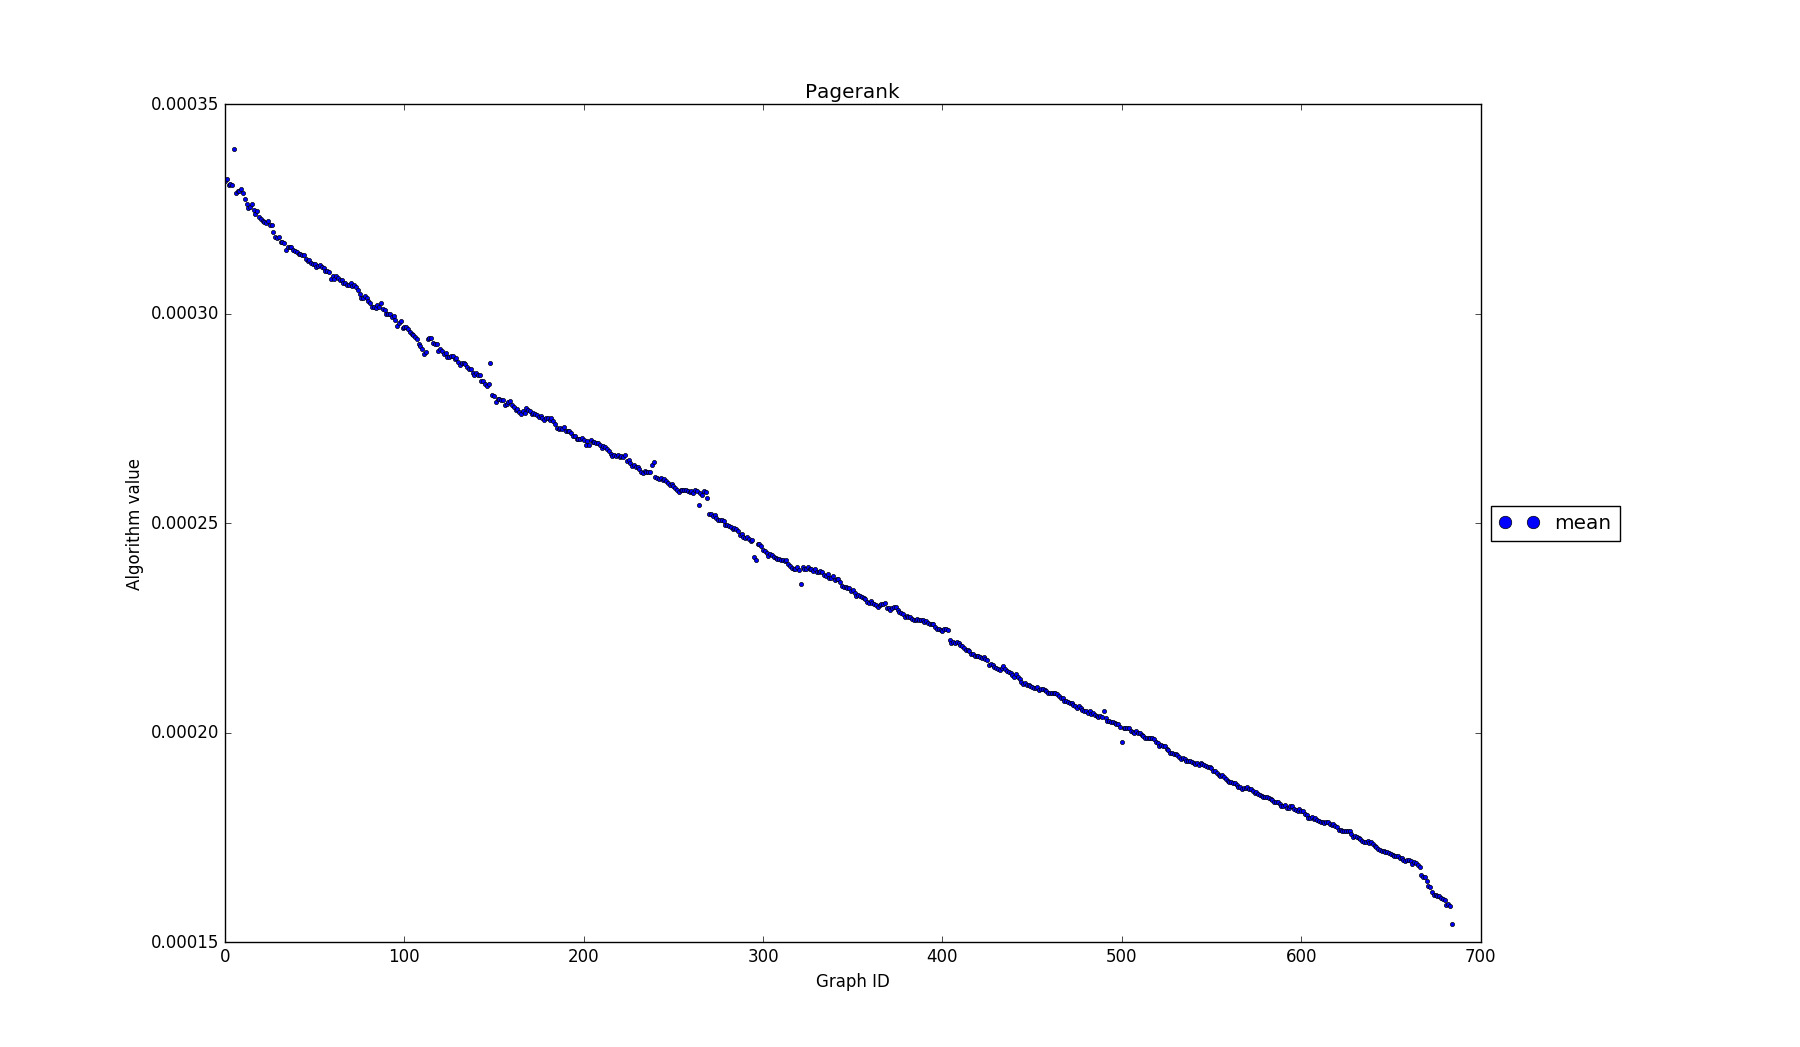
\includegraphics[width=\textwidth]{pagerank_mean}
	\caption{Średnie wartości pagerank}
\end{figure}
\FloatBarrier\FloatBarrier
\begin{figure}[h]
	\centering
	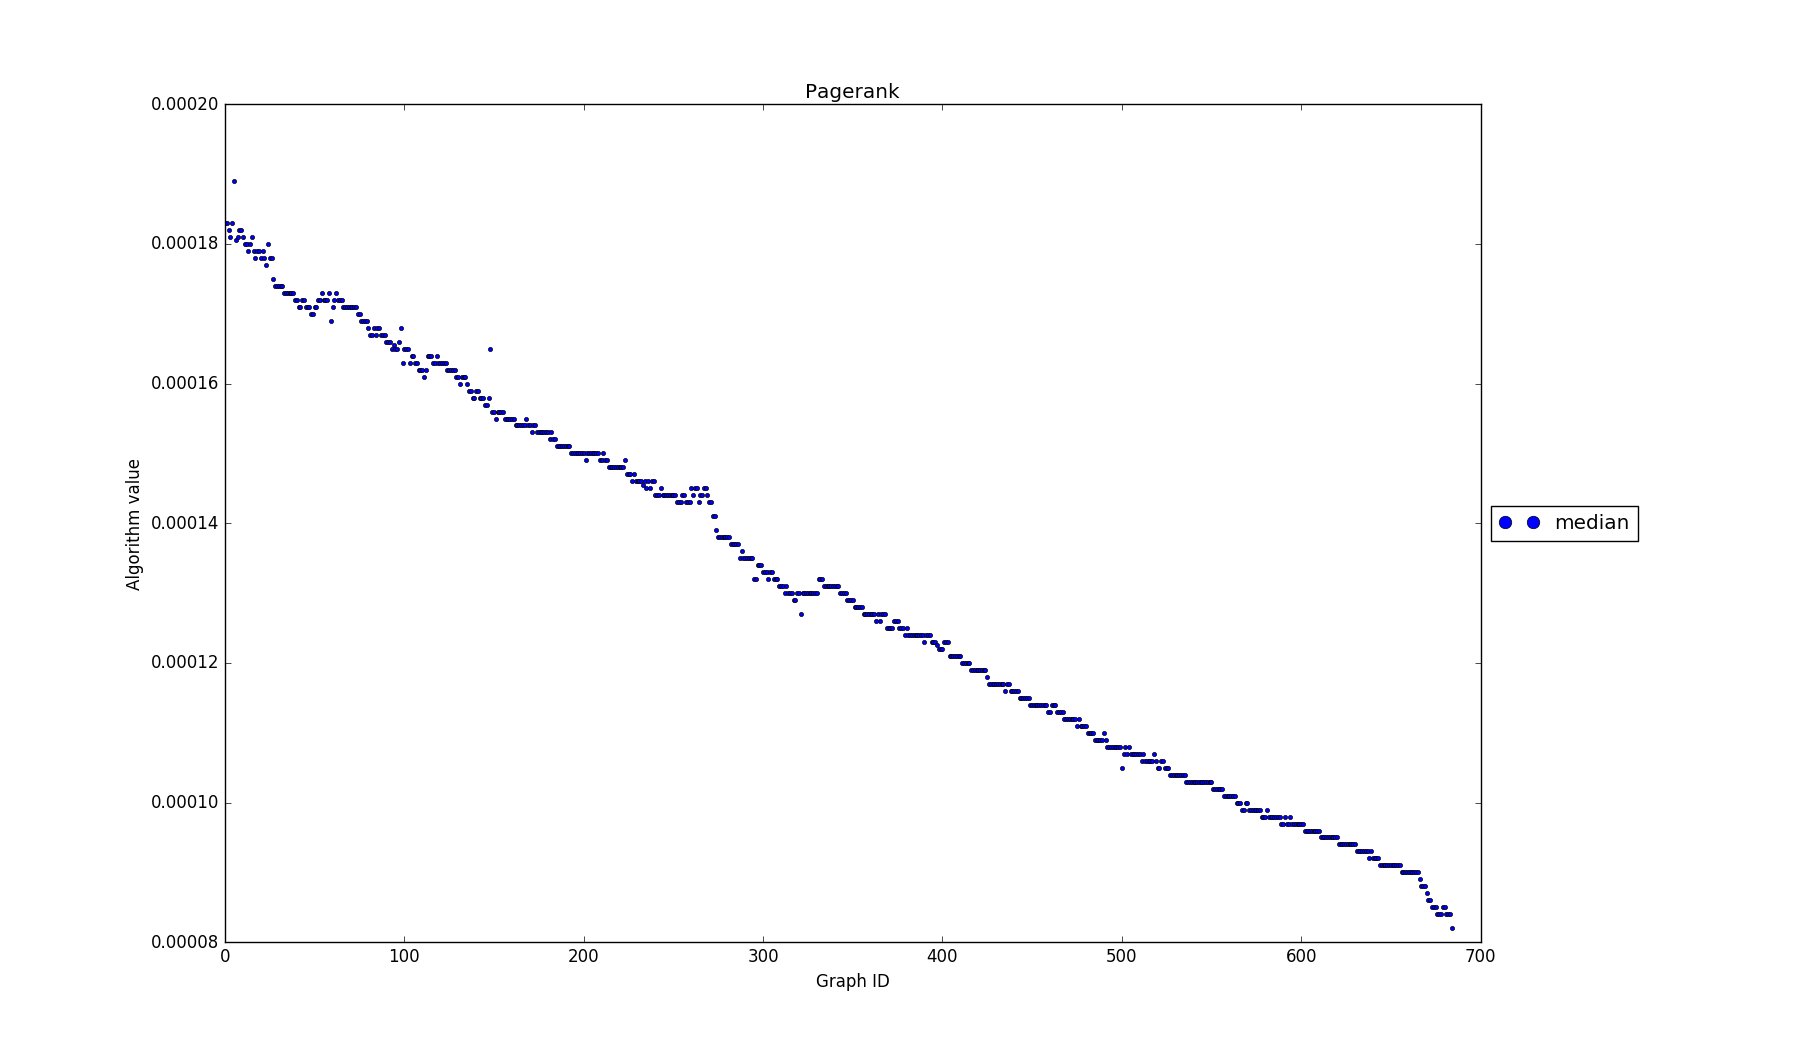
\includegraphics[width=\textwidth]{pagerank_median}
	\caption{Mediana wartości pagerank}
\end{figure}
Pagerank jest miarą tego jak dużo innych wierzchołków odwołuje się do badanego. Nie jest to równoznaczne ze stopniem wierzchołka ale ma on duży wpływ na wynik. W badanym okresie gęstość sieci malała, co daje się zauważyć również w spadku średniego wyniku algorytmu. Mimo tego maksymalna wartość pagerank, mimo drobnych fluktuacji, zachowuje podobny poziom. Wskazuje to na to, że nowe wierzchołki były w dużej mierze dodawane na obrzeżach a nie w środku sieci.
\FloatBarrier
\newpage

\chapter{Wizualizacja sieci}

Na potrzeby projektu intensywnie poszukiwano metod skutecznego wizualizowania badanych sieci. Przetestowaliśmy większość dostępnych narzędzi, w tym bardzo popularne oprogramowanie Gephi oraz bibliotekę NetworkX. Niestety, ze względu na znaczną wielkość grafów, żadne z łatwo dostępnych narzędzi nie umożliwiało stworzenia ich interaktywnej animacji. W związku z tym zdecydowano się na dwie, uzupełniające się metody.

\section{Graph-tool draw}

Pierwszą z nich jest funkcja rysująca z biblioteki Graph-tool. Posiada ona szerokie możliwości odnośnie formy wyjściowej rysowanych grafów. Okno interaktywne nie zapewniało odpowiedniej płynności animacji, co w praktyce uniemożliwiało korzystanie z niego. Zadowalająca z kolei okazała się możliwość generacji statycznych obrazów PNG w dużej rozdzielczości. Maksymalna rozdzielczość nie była ograniczona przez bibliotekę, z sukcesem generowano obrazy 20 000 x 20 000 pixeli. Jednakże ilość pamięci operacyjnej na dostępnym sprzęcie testowym narzucała ograniczenie na rozdzielczość i w efekcie zdecydowano się na 10 000 x 10 000. Zapewnia to odpowiednią ostrość nawet przy dużym powiększeniu.
 
Funkcja udostępniała kolorowanie grafu i zmianę rozmiarów jego wierzchołków zgodnie z wyliczoną miarą centralności. Kolorowanie odbywało się według skali \textit{gnuplot}, im wartość miary była większa, tym kolor był cieplejszy (bliżej żółtego).

\FloatBarrier\FloatBarrier
\begin{figure}[h]
	\centering
	
\includegraphics[width=\textwidth]{colormaps_reference_05.png}
	\caption{Użyta mapa koloru}
\end{figure}
\FloatBarrier\FloatBarrier

Poniżej znajdują się wizualizacje dla wszystkich 3 algorytmów dla najstarszego grafu (1997 rok) oraz najmłodszego (2000 rok).

\FloatBarrier\FloatBarrier
\begin{figure}[h]
	\centering
	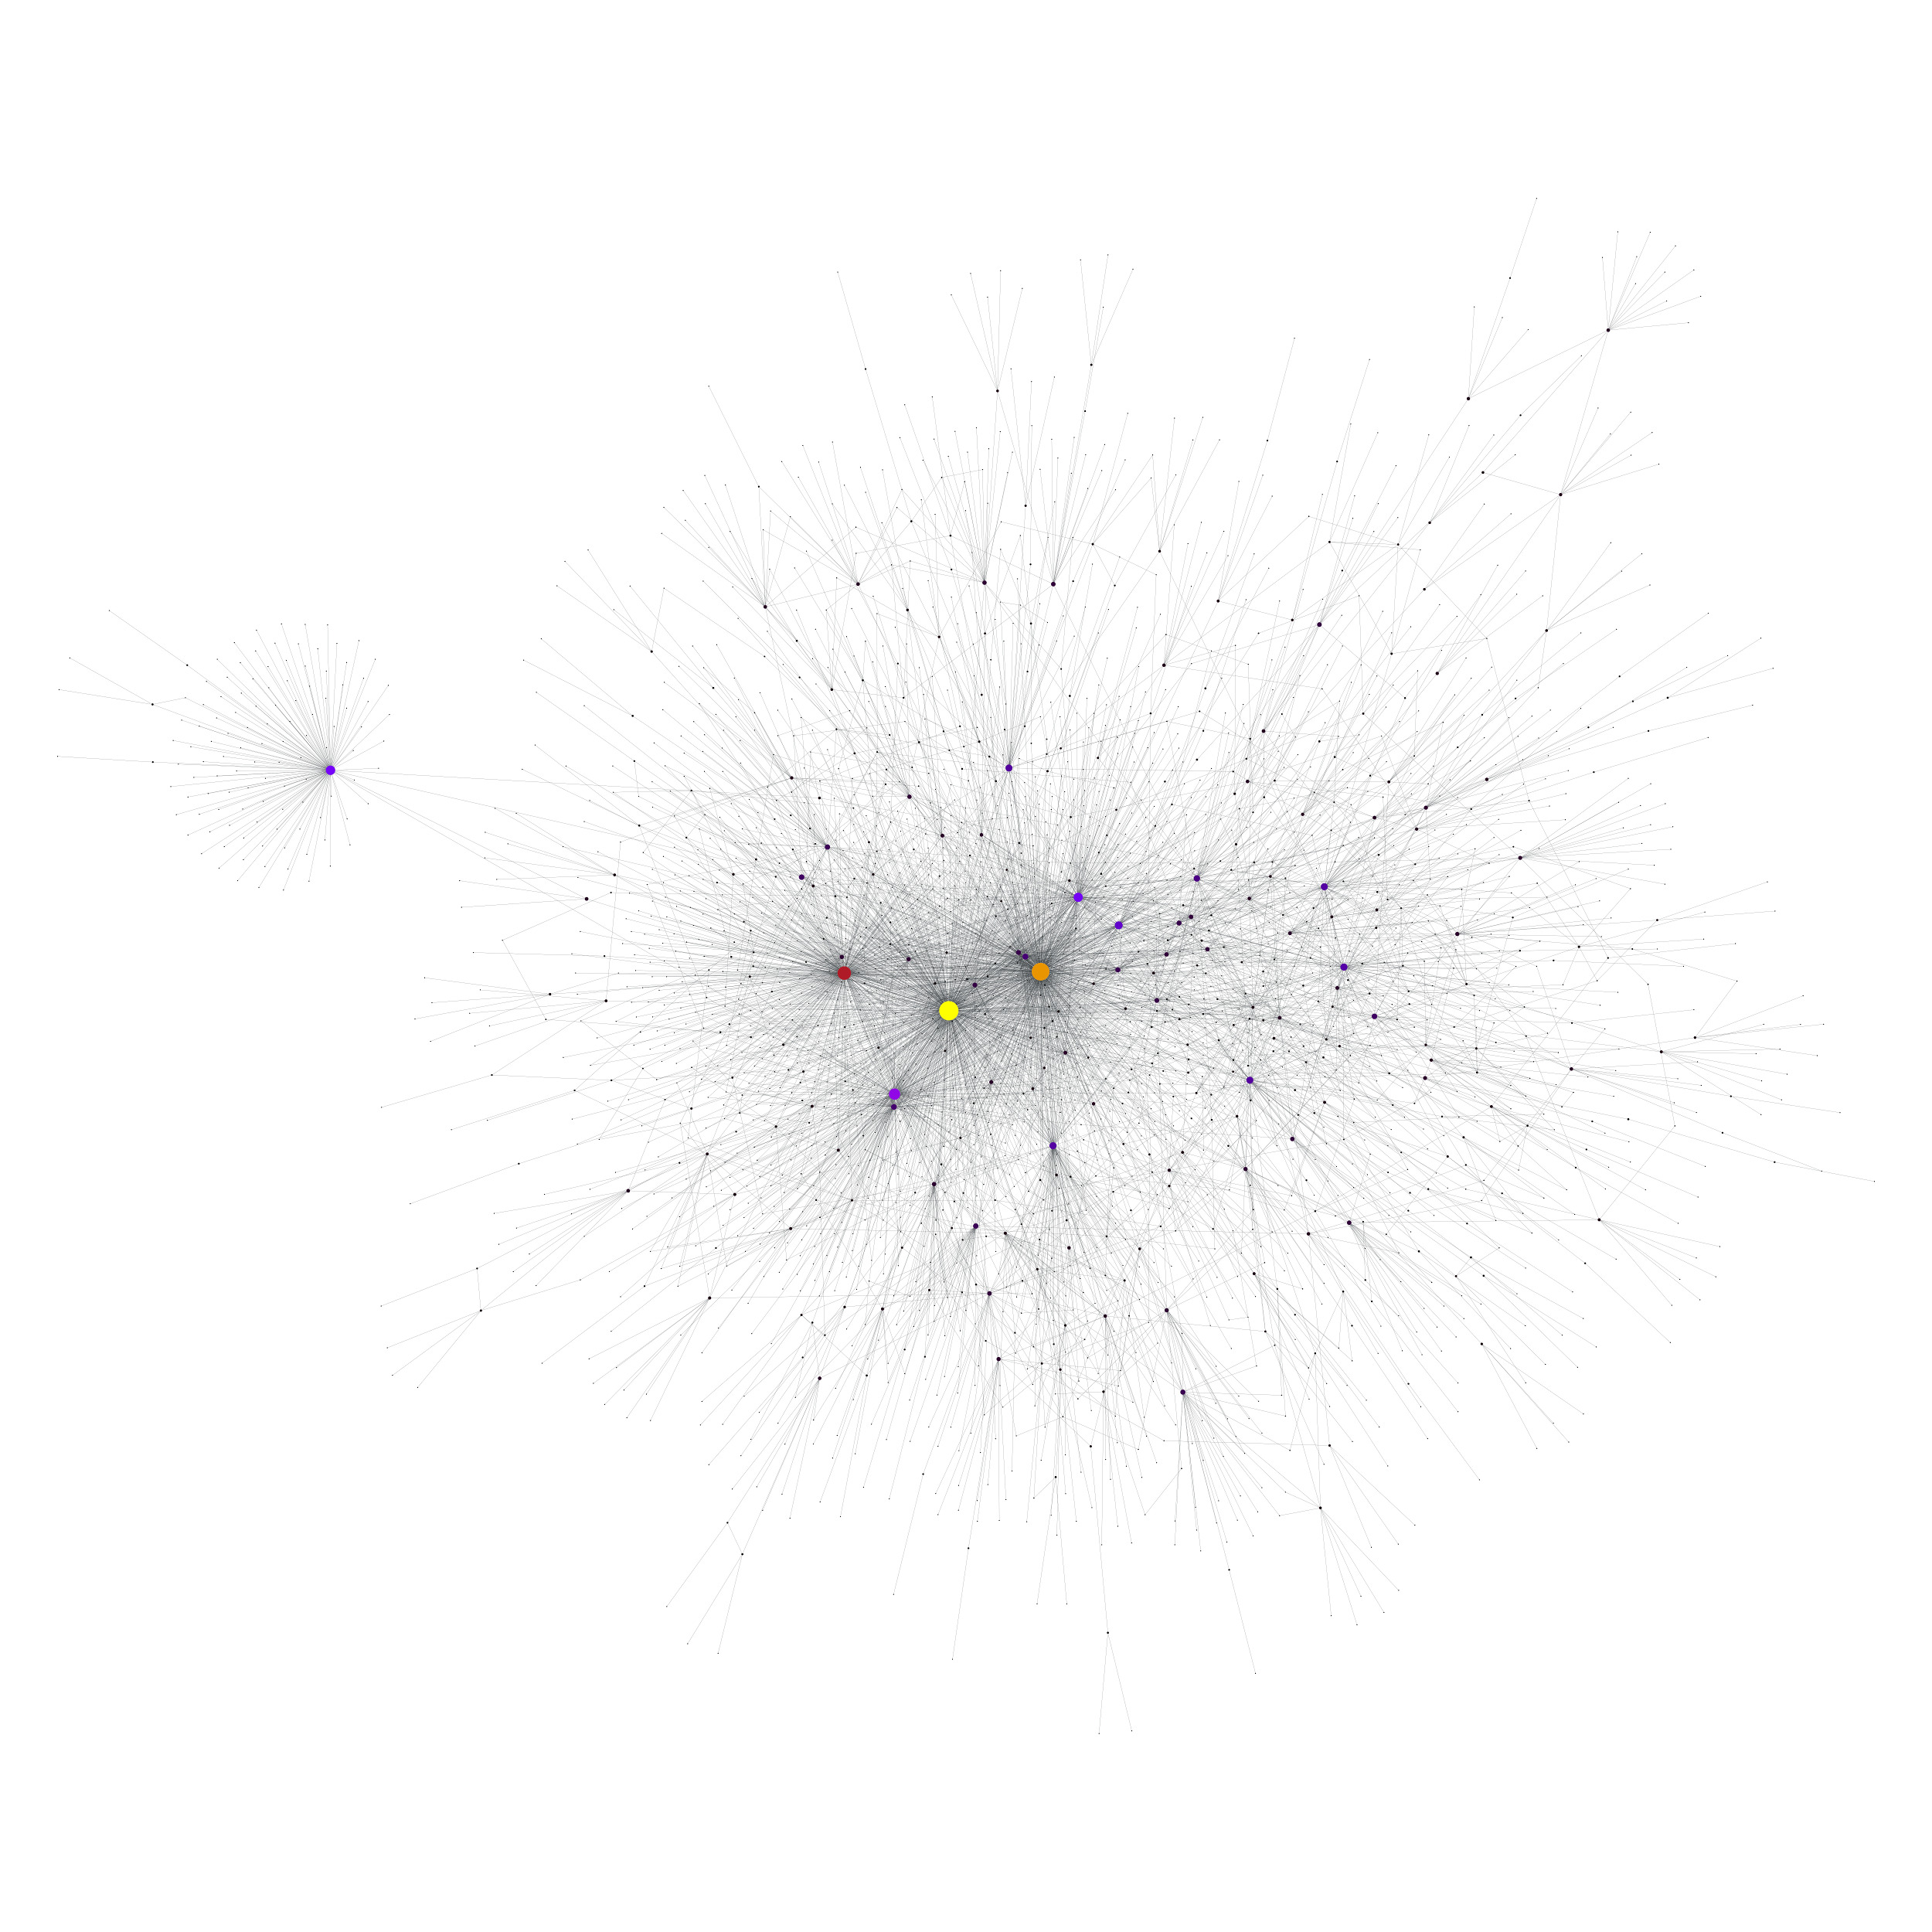
\includegraphics[width=\textwidth]{3015_betweenness.png}
	\caption{Graf z początku zebranego zestawu danych dla algorytmu betweenness}
\end{figure}
\FloatBarrier\FloatBarrier

\FloatBarrier\FloatBarrier
\begin{figure}[h]
	\centering
	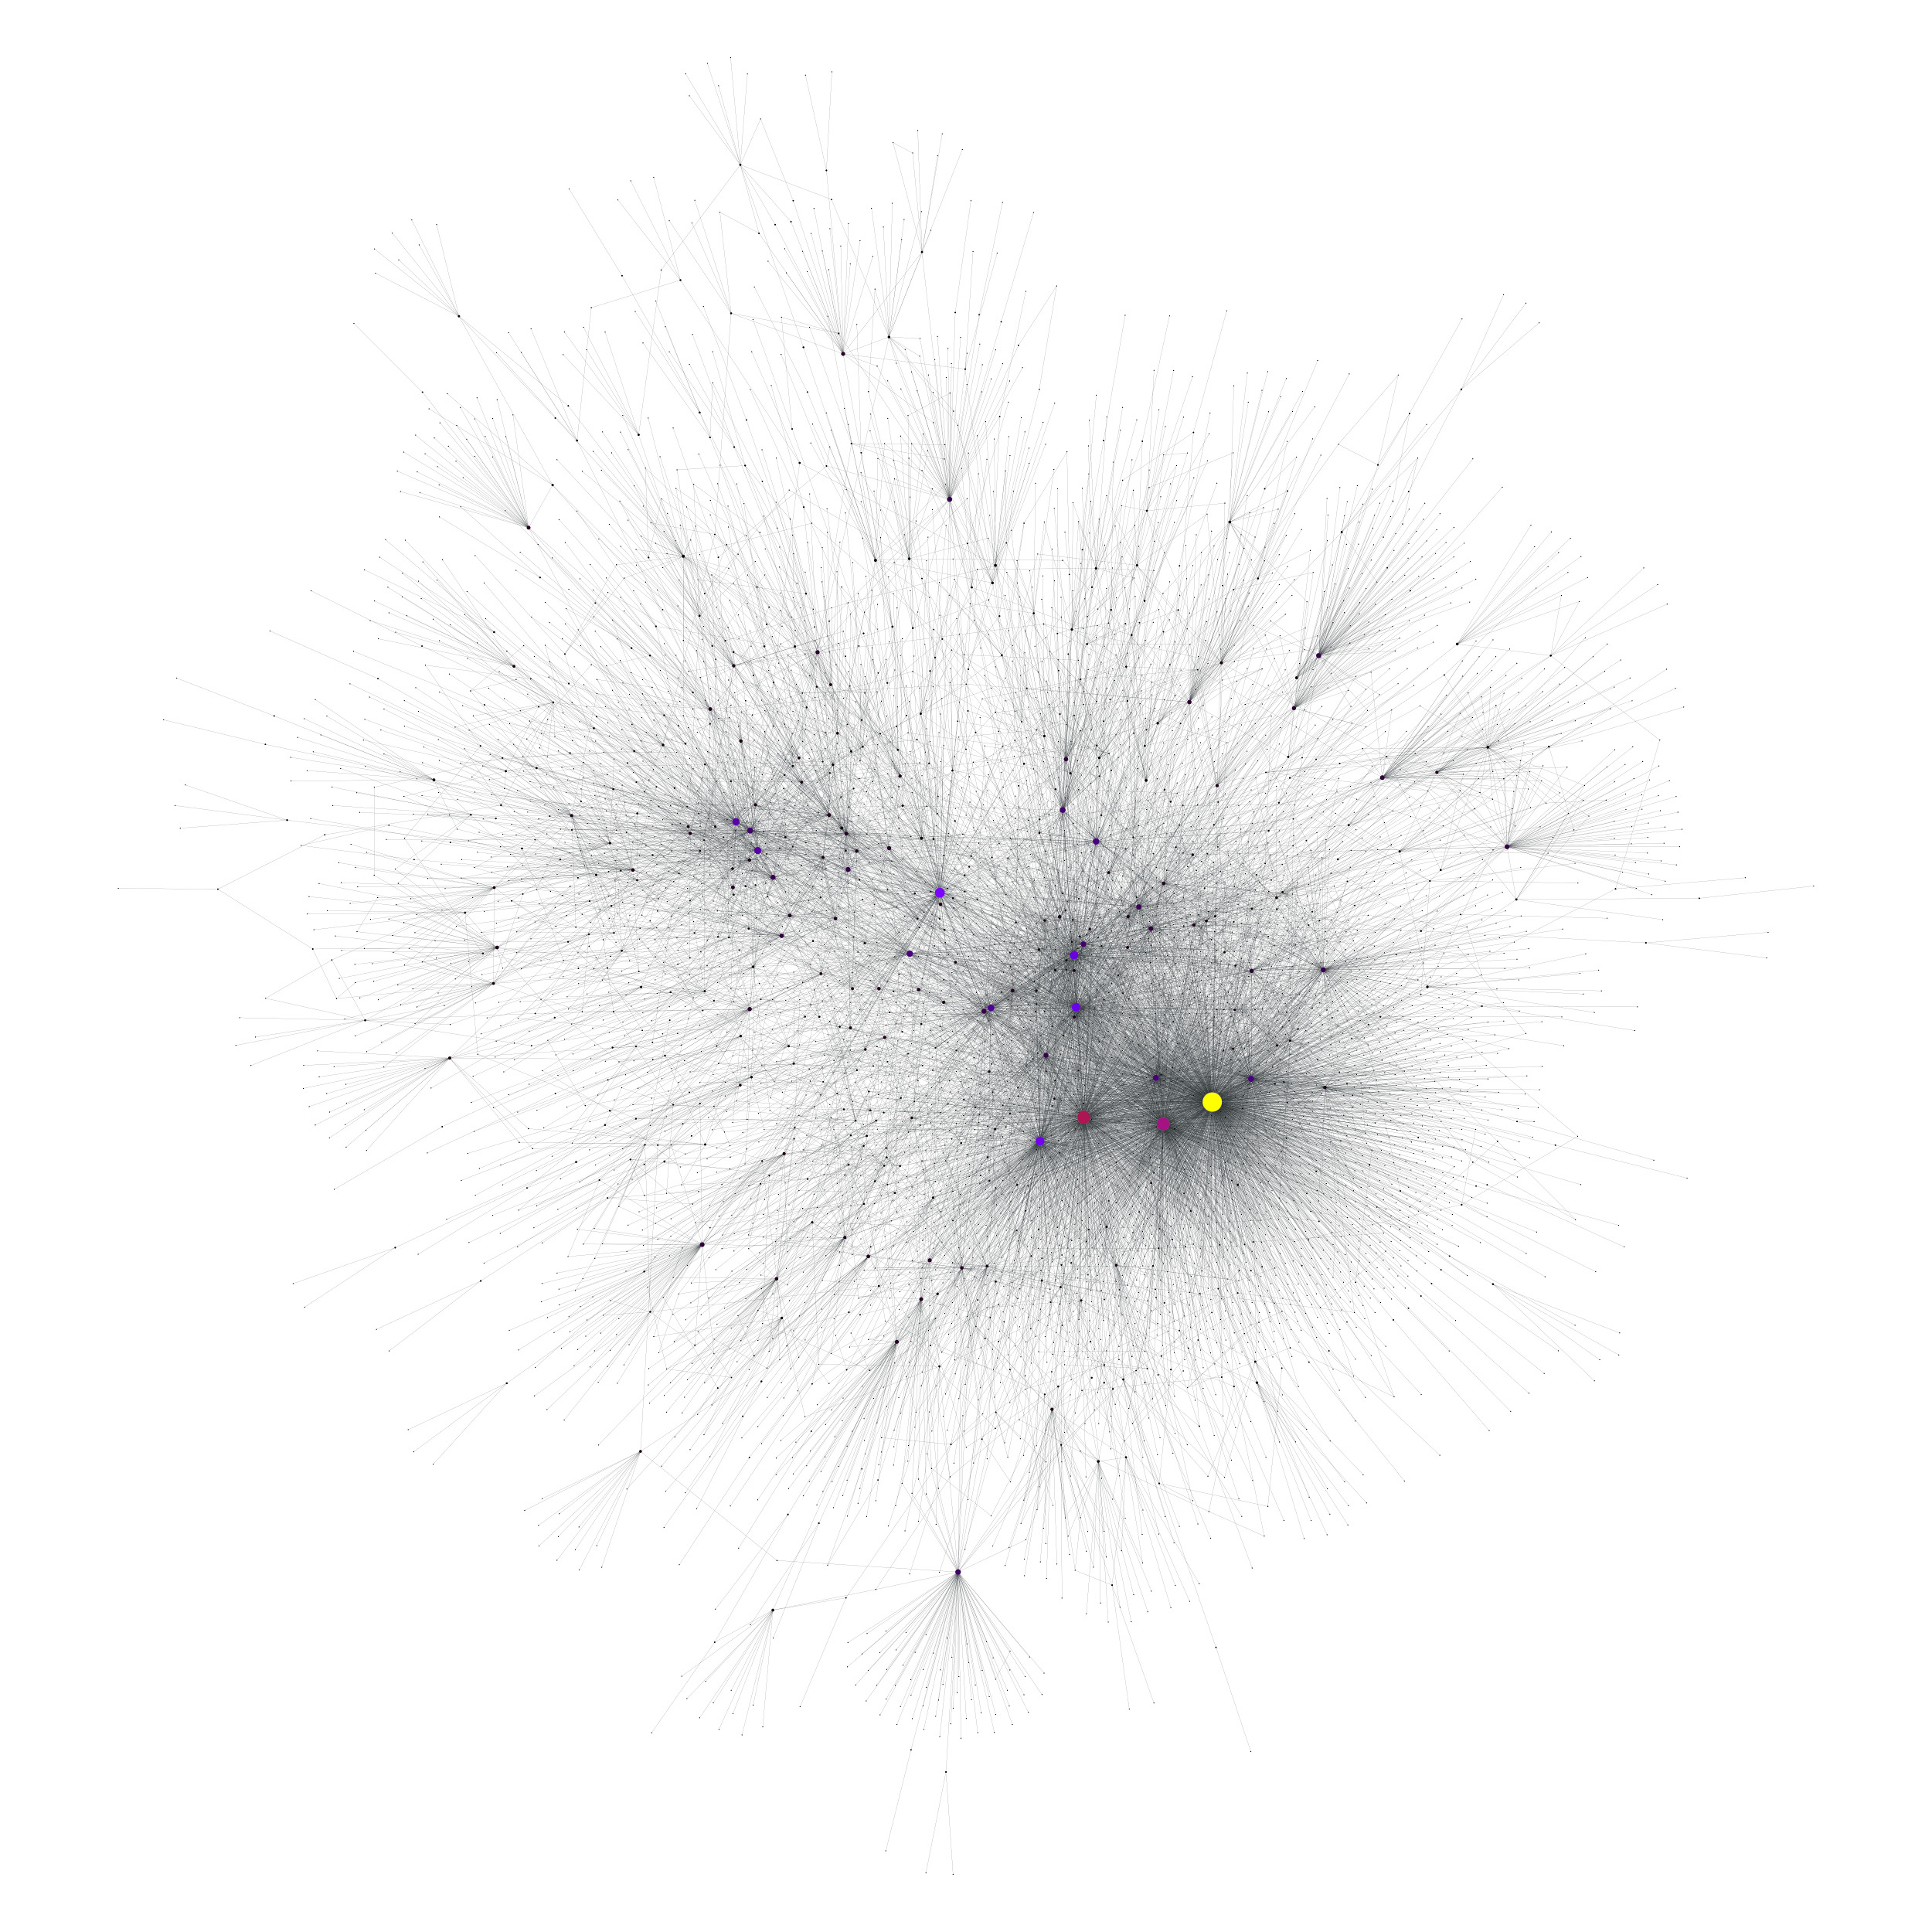
\includegraphics[width=\textwidth]{6474_betweenness.png}
	\caption{Graf z końca zebranego zestawu danych dla algorytmu betweenness}
\end{figure}
\FloatBarrier\FloatBarrier

\FloatBarrier\FloatBarrier
\begin{figure}[h]
	\centering
	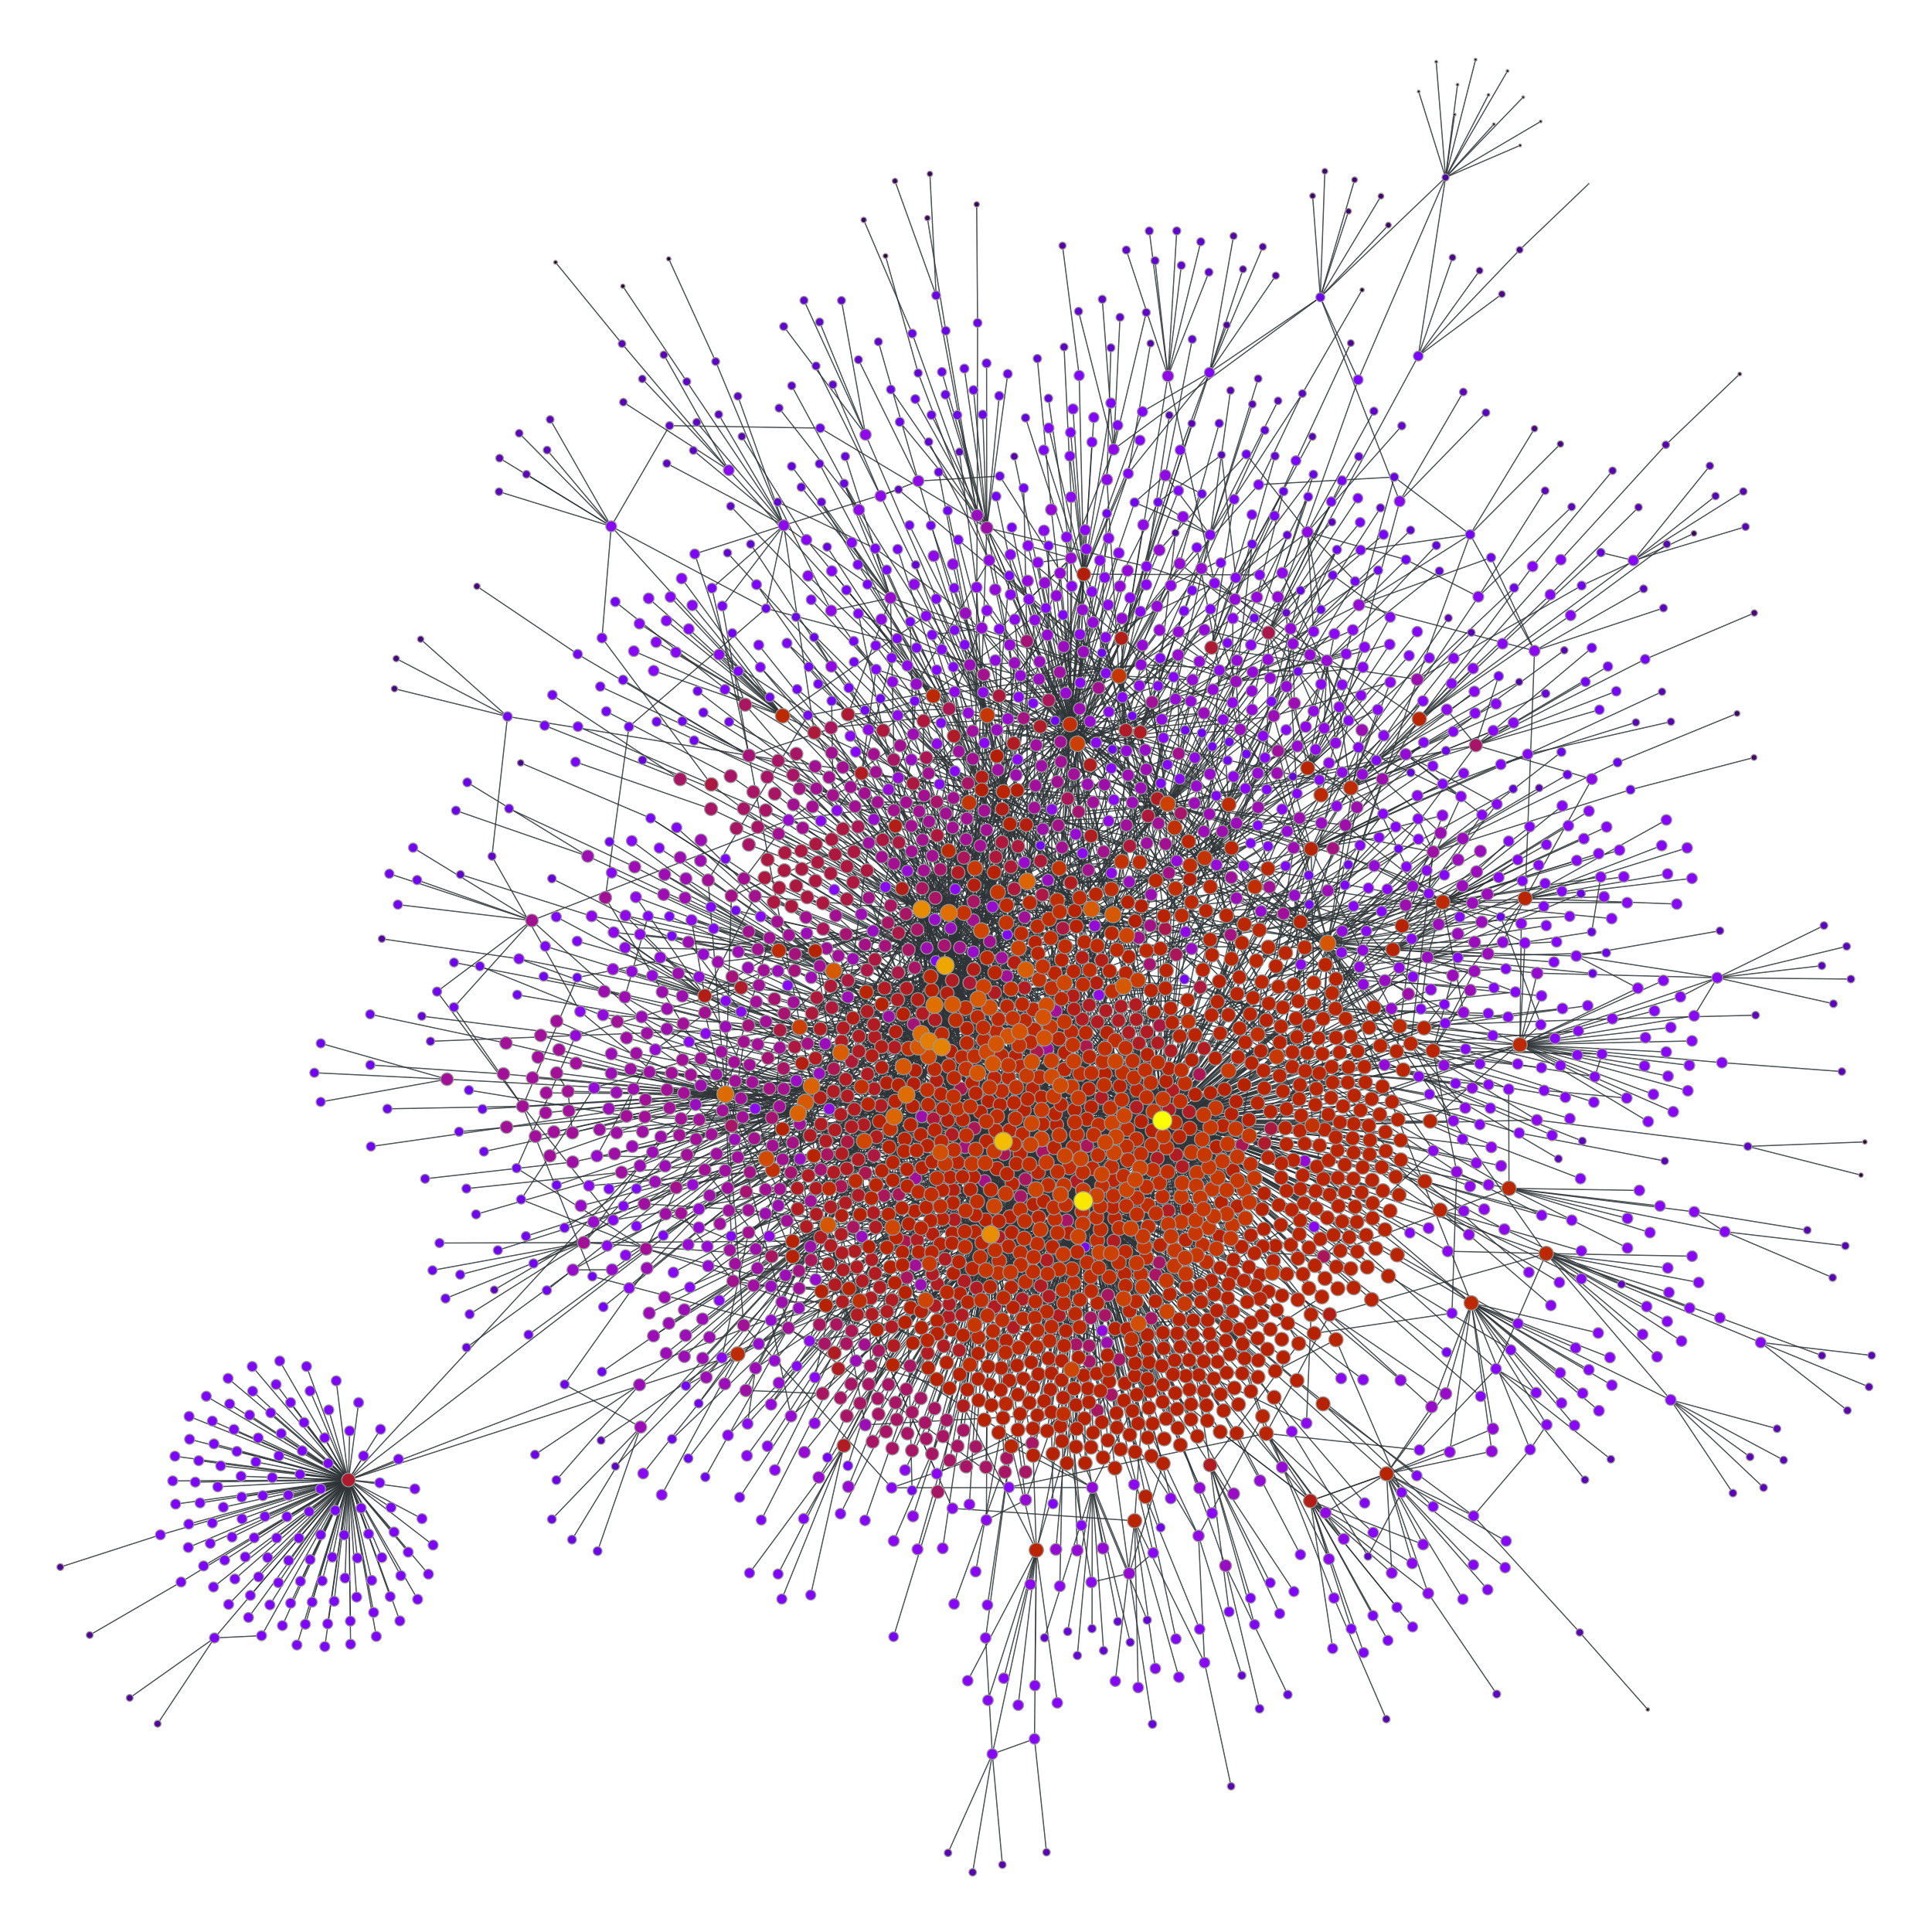
\includegraphics[width=\textwidth]{3015_closeness.png}
	\caption{Graf z początku zebranego zestawu danych dla algorytmu closeness}
\end{figure}
\FloatBarrier\FloatBarrier

\FloatBarrier\FloatBarrier
\begin{figure}[h]
	\centering
	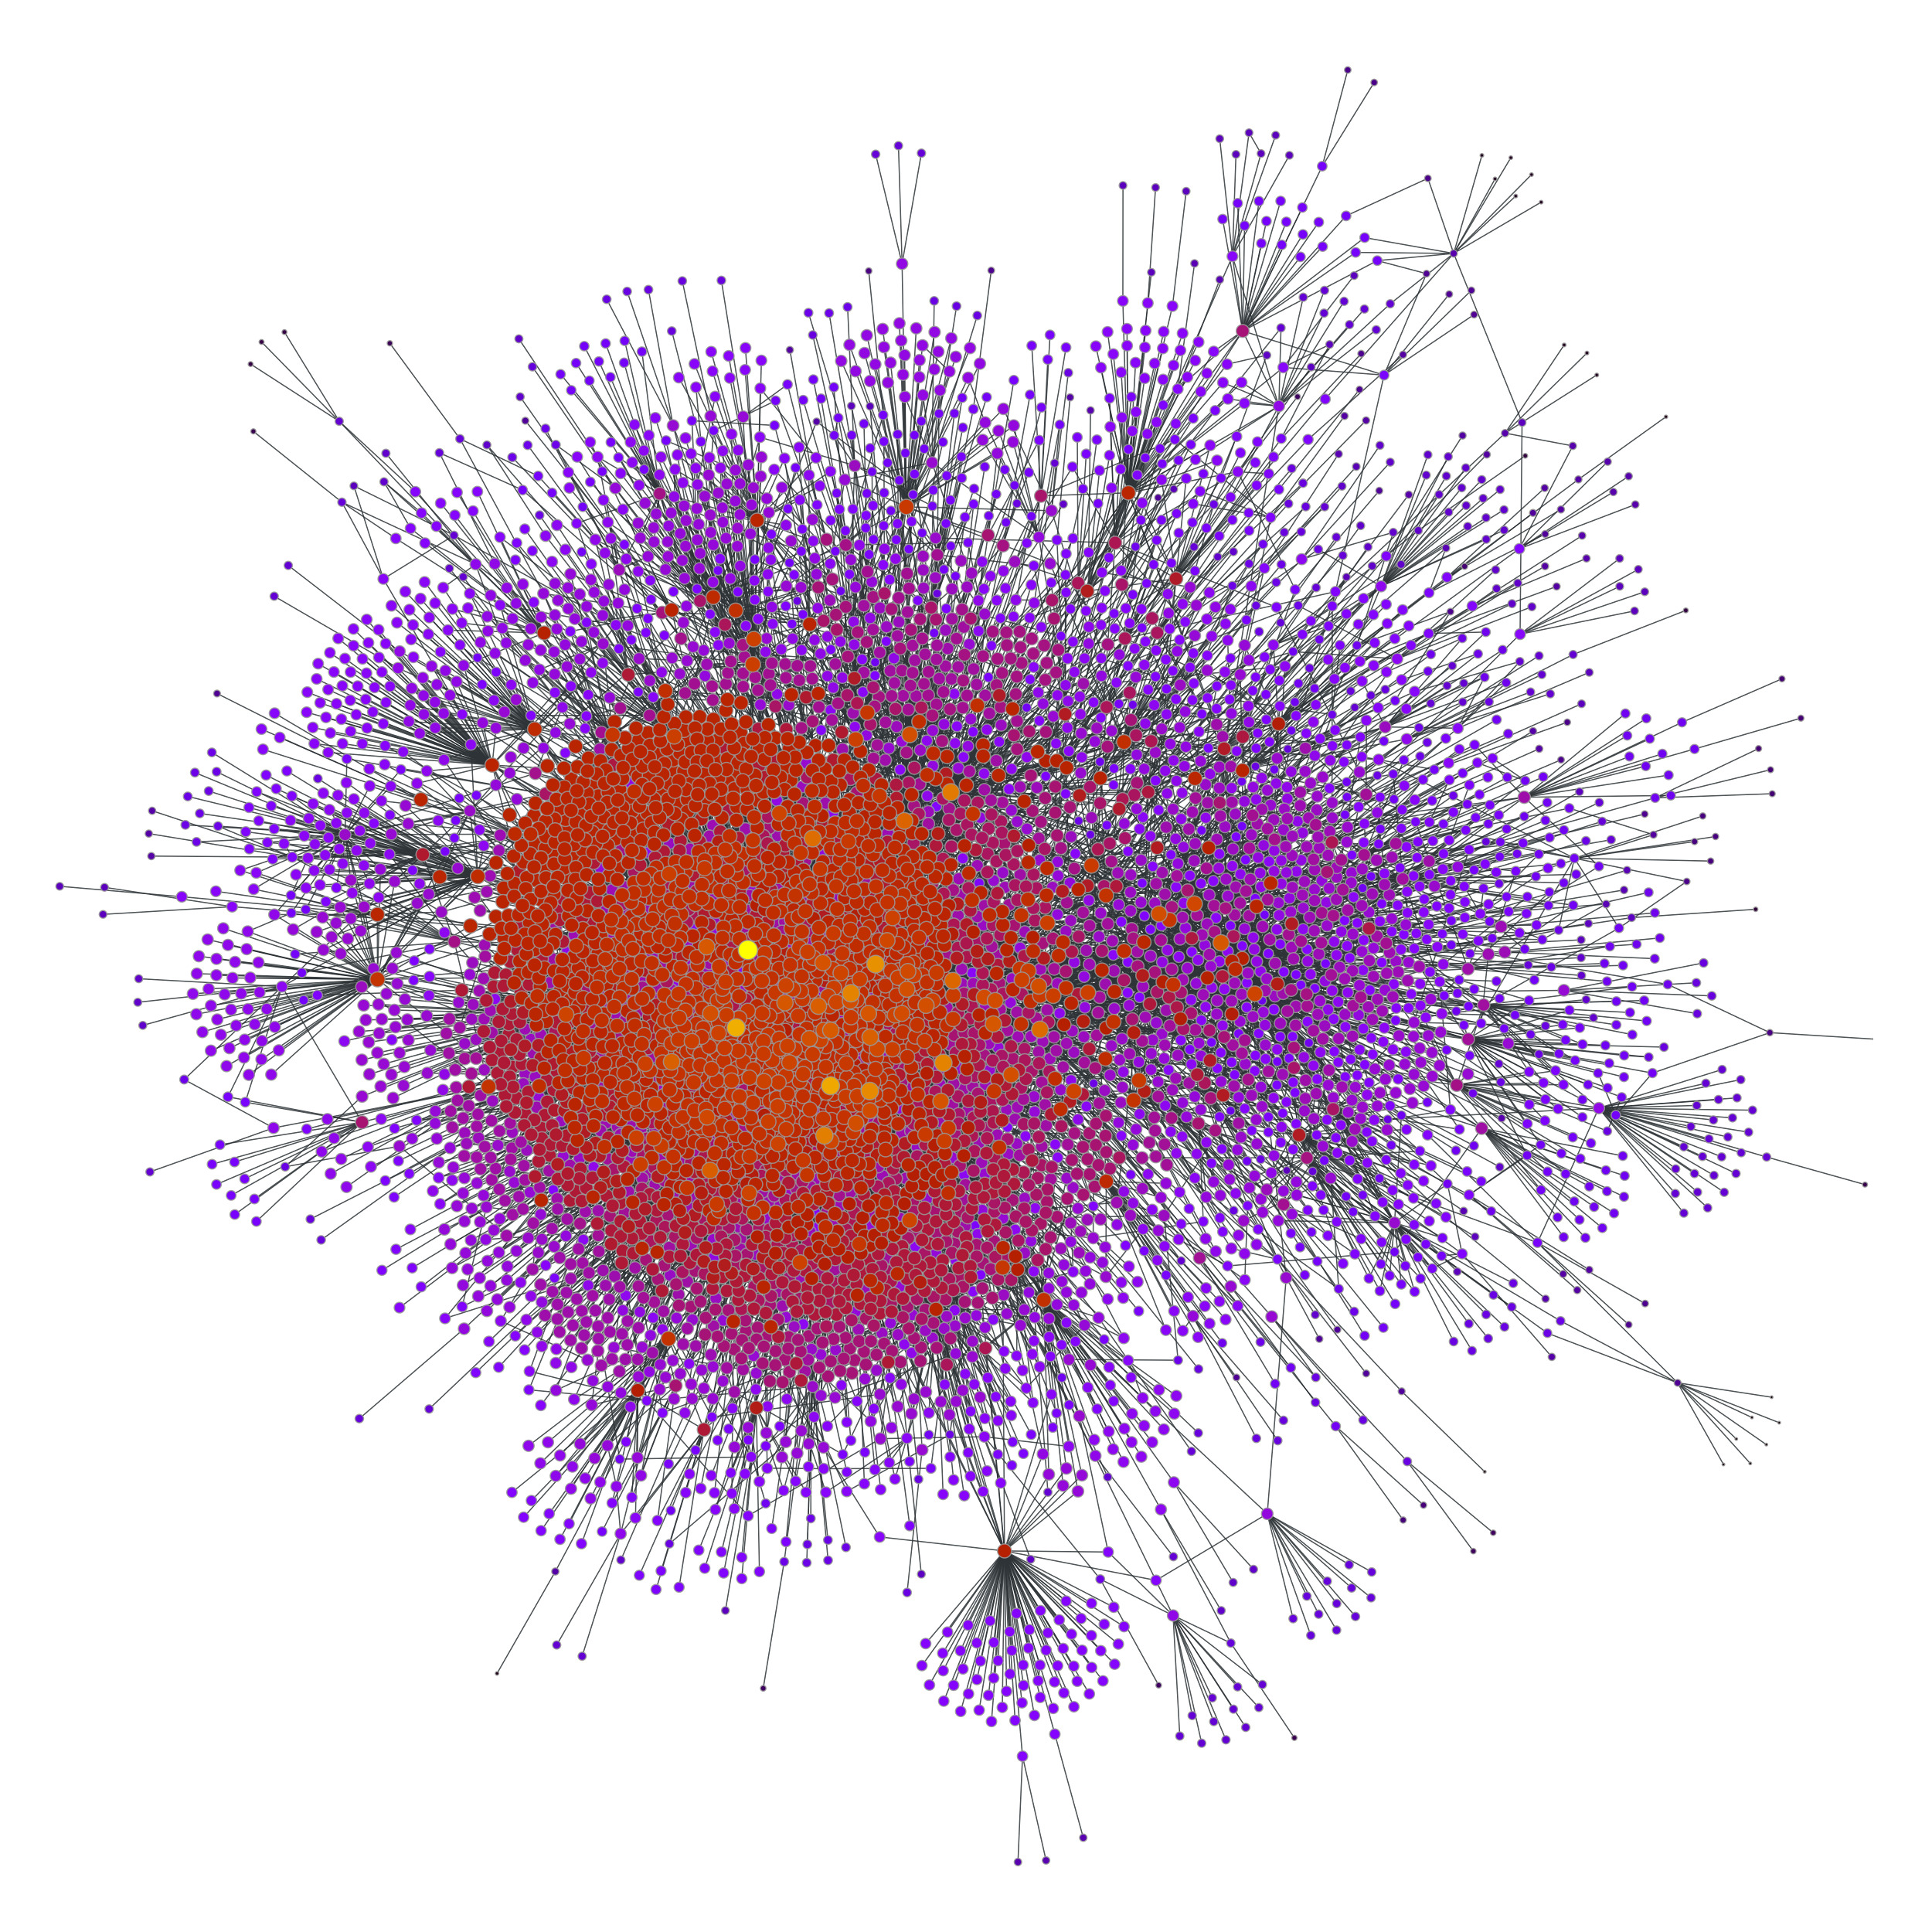
\includegraphics[width=\textwidth]{6474_closeness.png}
	\caption{Graf z końca zebranego zestawu danych dla algorytmu closeness}
\end{figure}
\FloatBarrier\FloatBarrier

\FloatBarrier\FloatBarrier
\begin{figure}[h]
	\centering
	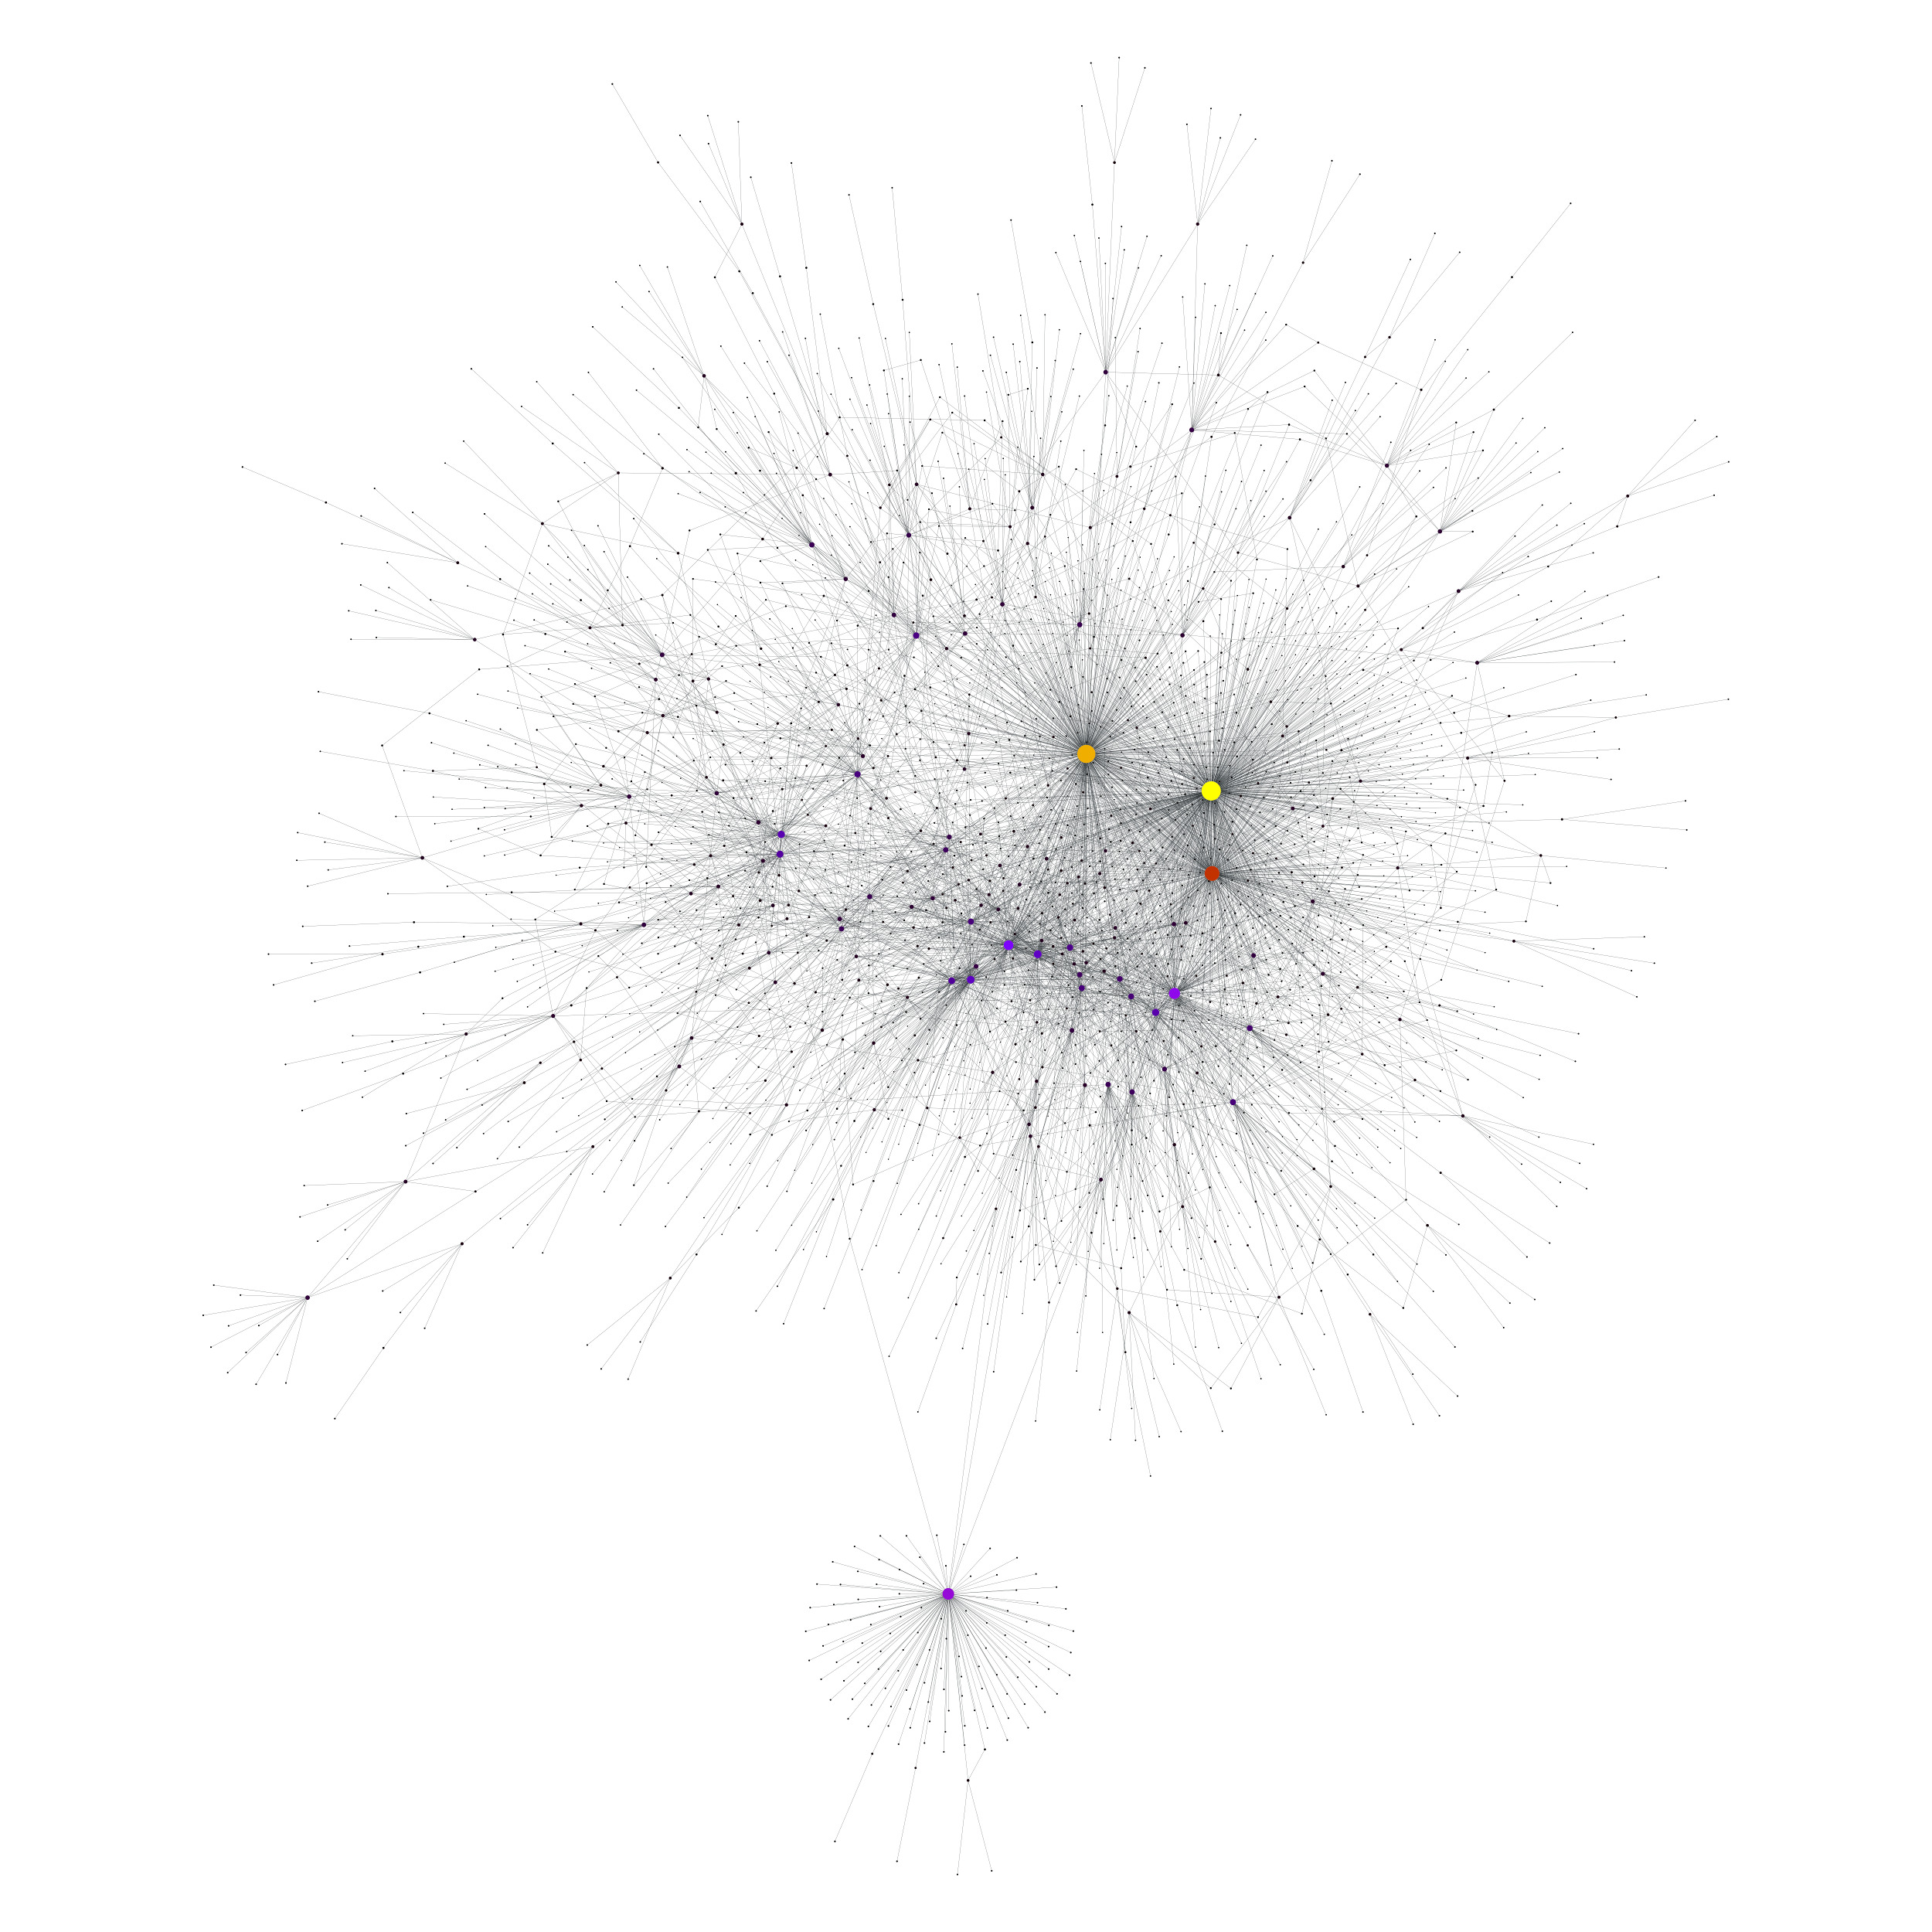
\includegraphics[width=\textwidth]{3015_pagerank.png}
	\caption{Graf z początku zebranego zestawu danych dla algorytmu pagerank}
\end{figure}
\FloatBarrier\FloatBarrier

\FloatBarrier\FloatBarrier
\begin{figure}[h]
	\centering
	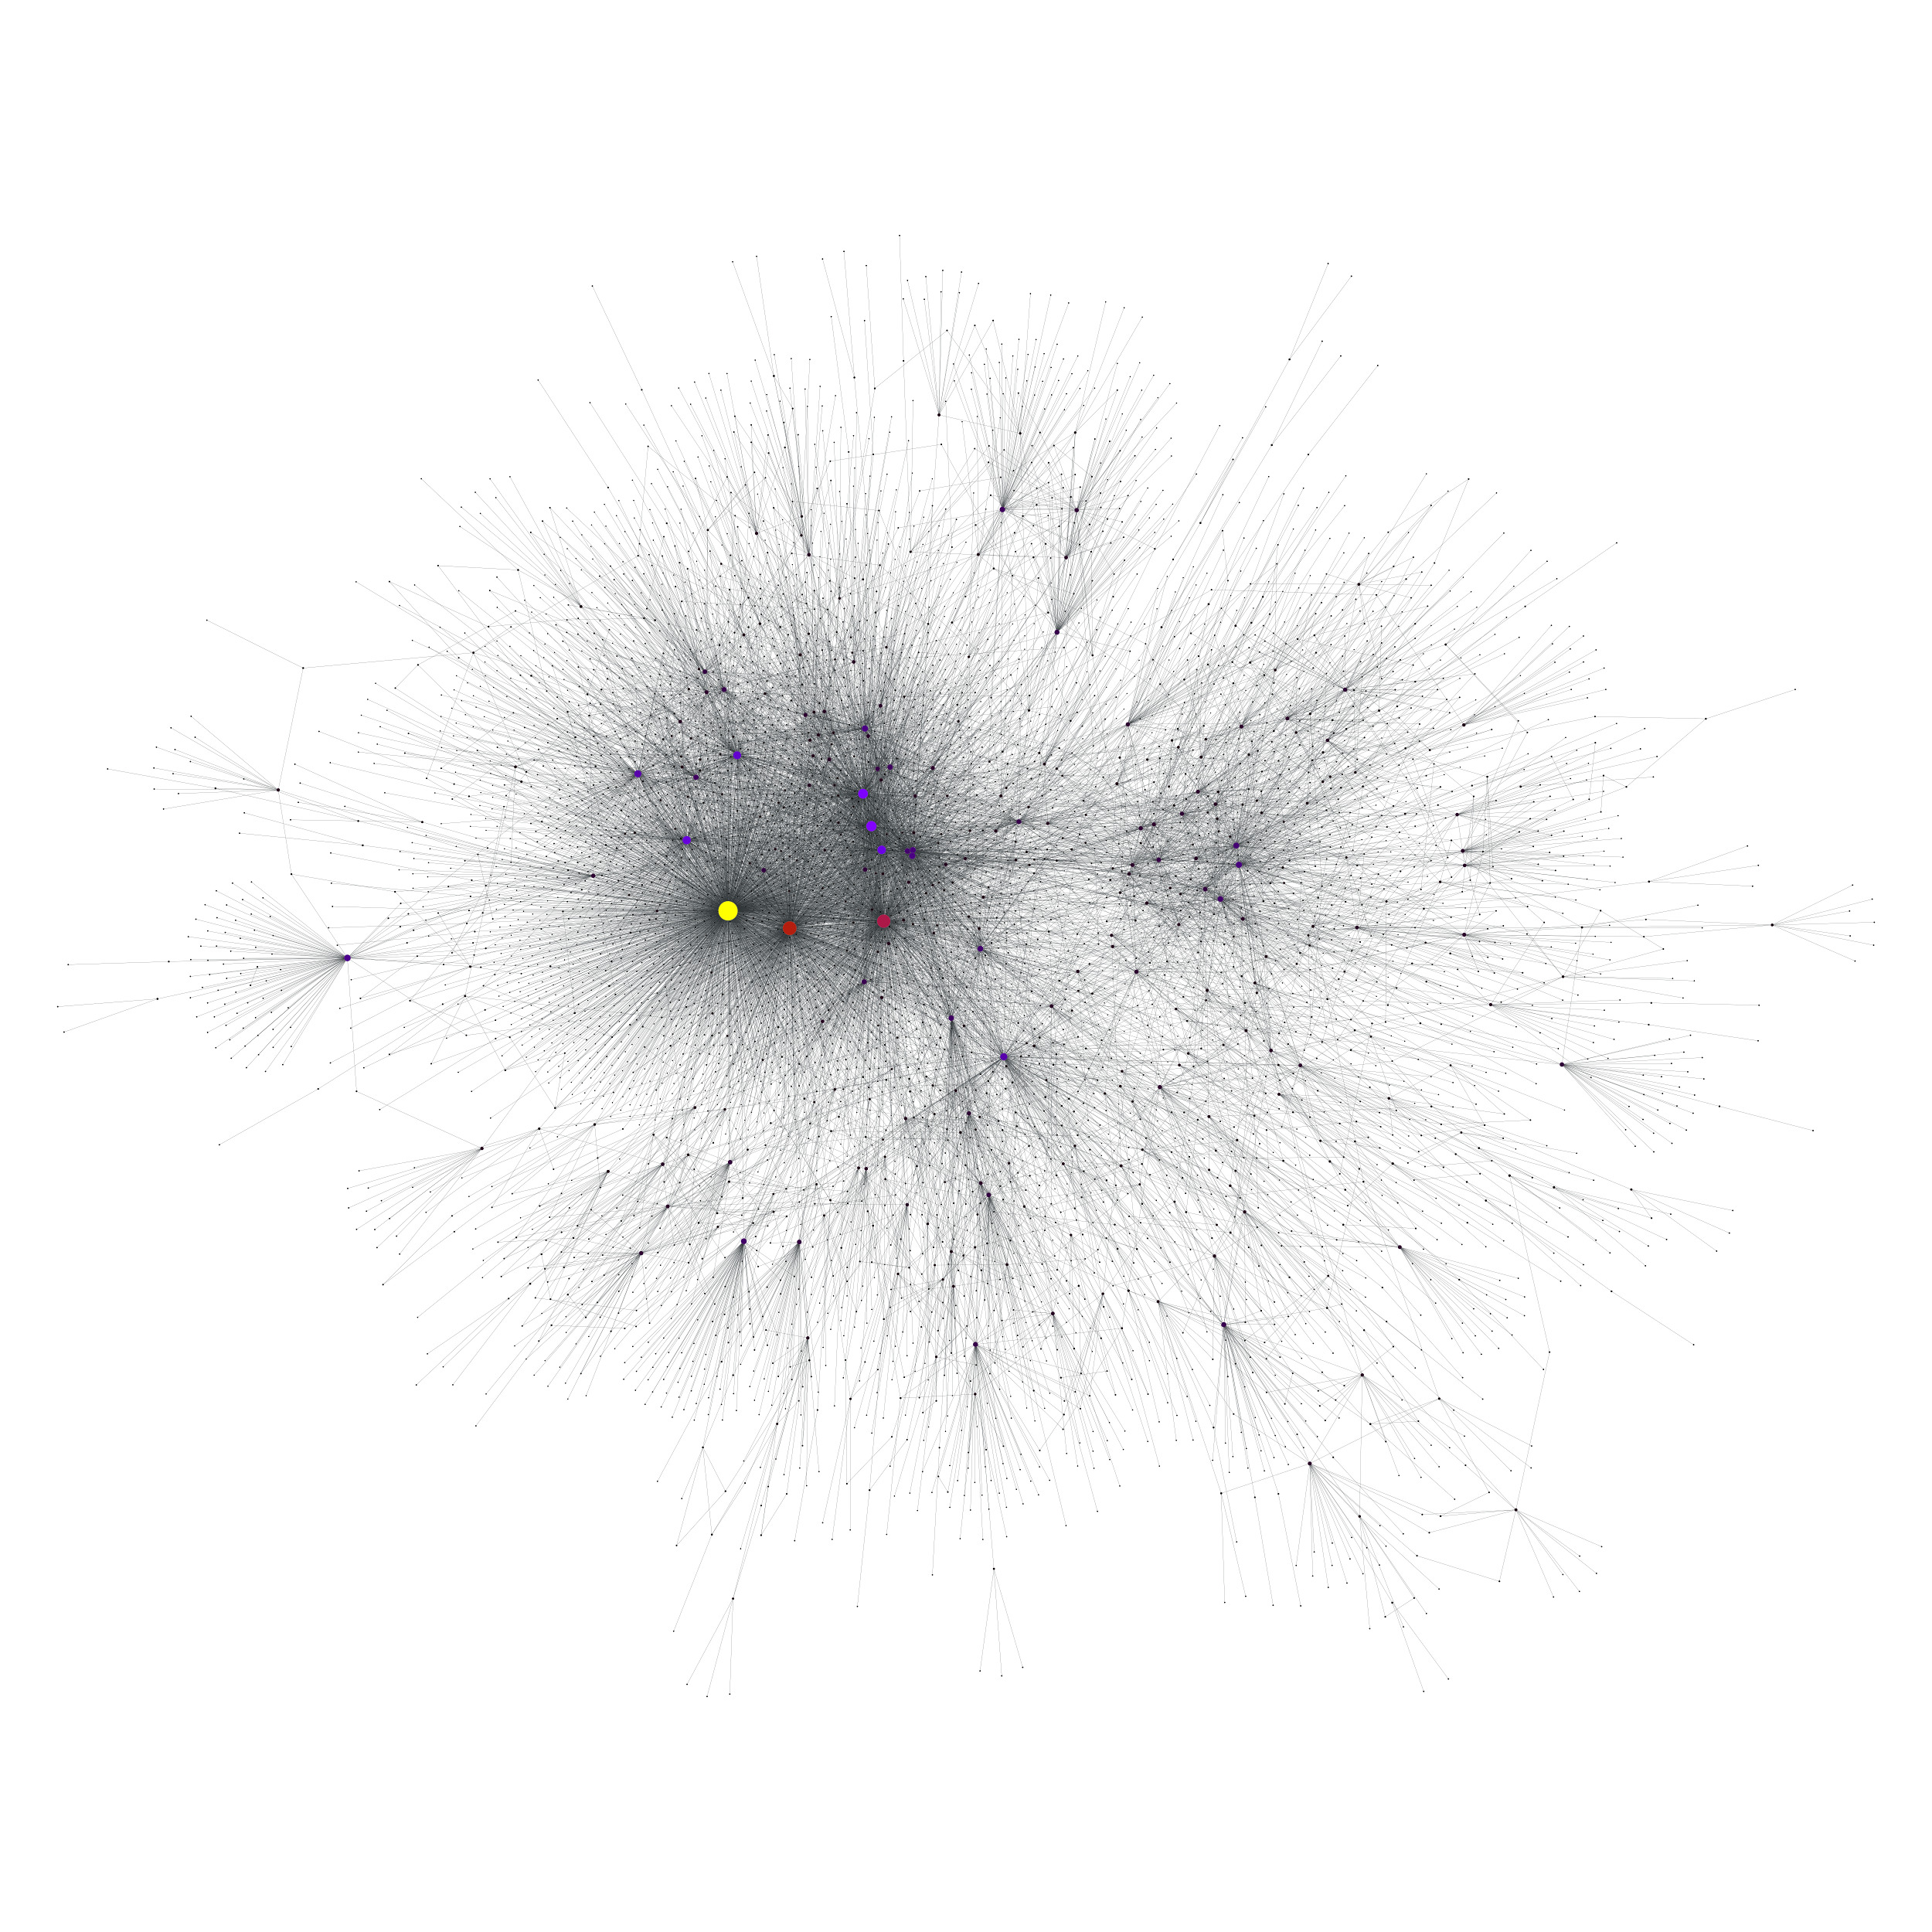
\includegraphics[width=\textwidth]{6474_pagerank.png}
	\caption{Graf z końca zebranego zestawu danych dla algorytmu pagerank}
\end{figure}
\FloatBarrier\FloatBarrier

\section{Walrus}

Druga metoda wizualizacji opierała się na oprogramowaniu Walrus, stworzonym w okolicach 2000 roku przez organizację CAIDA, zajmującą się badaniem topologii sieci. Jego rozwój zakończono w 2005 roku, mimo to jest to jedyne narzędzie będące w stanie interaktywnie zwizualizować bardzo duże grafy na stosunkowo słabym sprzęcie i to w przestrzeni trójwymiarowej. Mimo tych niewątpliwych zalet program jest toporny w użytkowaniu i nadaje się głównie do grafów zbliżonych do drzewa rozpinającego. Wymaga on pliku wsadowego w egzotycznym formacie LibSea, konieczne więc było napisanie specjalnego generatora. Do innych ograniczeń zaliczyć można: 
\begin{itemize}
\item obsługa wyłącznie grafów skierowanych
\item obsługa tylko grafów spójnych
\item podanie w pliku wsadowym pełnego drzewa rozpinającego
\item brak obsługi krawędzi wielokrotnych i cykli w grafie
\item brak obsługi pętli w grafie
\end{itemize}

Powyższe ograniczenia wymusiły dokonania transformacji grafu. Efekty widoczne są poniżej. Podobnie jak w pierwszej metodzie, kolory odpowiadają przeskalowanej wartości miar centralności. Kolorowane są również krawędzie, według zasady: krawędź łącząca dwa węzły przyjmuje kolor wierzchołka o większej przypisanej wartości miary. Zdecydowano się na takie rozwiązanie w celu zwiększenia widoczności wierzchołków. Z tego samego powodu poniższe wizualizacje zawierają tylko drzewo spinające badanych grafów. Ostania obejmuje cały graf w celach porównawczych. 

\FloatBarrier\FloatBarrier
\begin{figure}[h]
	\centering
	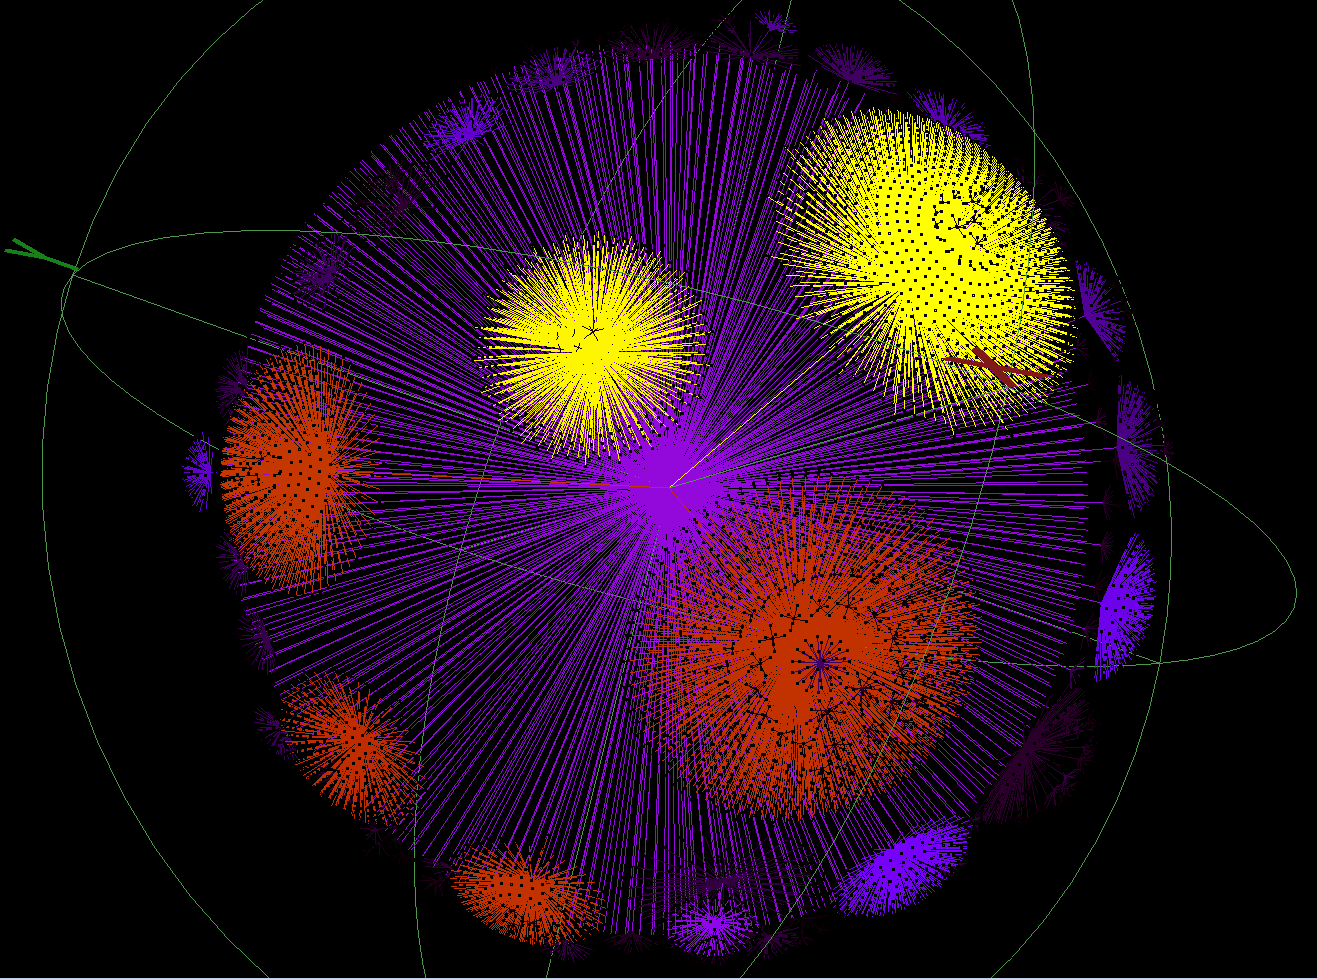
\includegraphics[width=\textwidth]{Betweenness_walrus.png}
	\caption{Najstarszy graf, wizualizacja algorytmu betweenness}
\end{figure}
\FloatBarrier\FloatBarrier
\FloatBarrier\FloatBarrier
\begin{figure}[h]
	\centering
	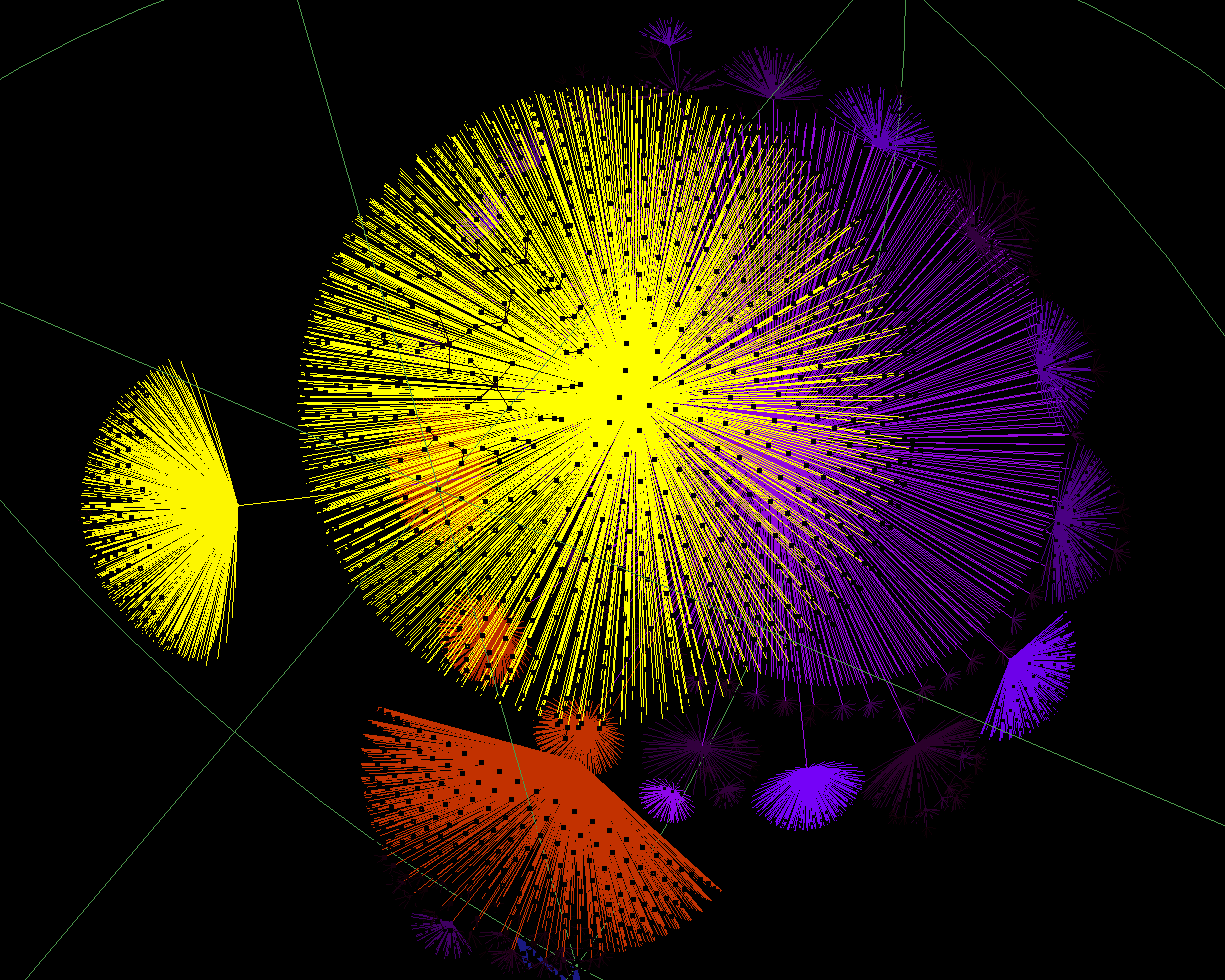
\includegraphics[width=\textwidth]{Betweenness2_walrus.png}
	\caption{Najstarszy graf, wizualizacja algorytmu betweenness - ujęcie 2}
\end{figure}
\FloatBarrier\FloatBarrier

\FloatBarrier\FloatBarrier
\begin{figure}[h]
	\centering
	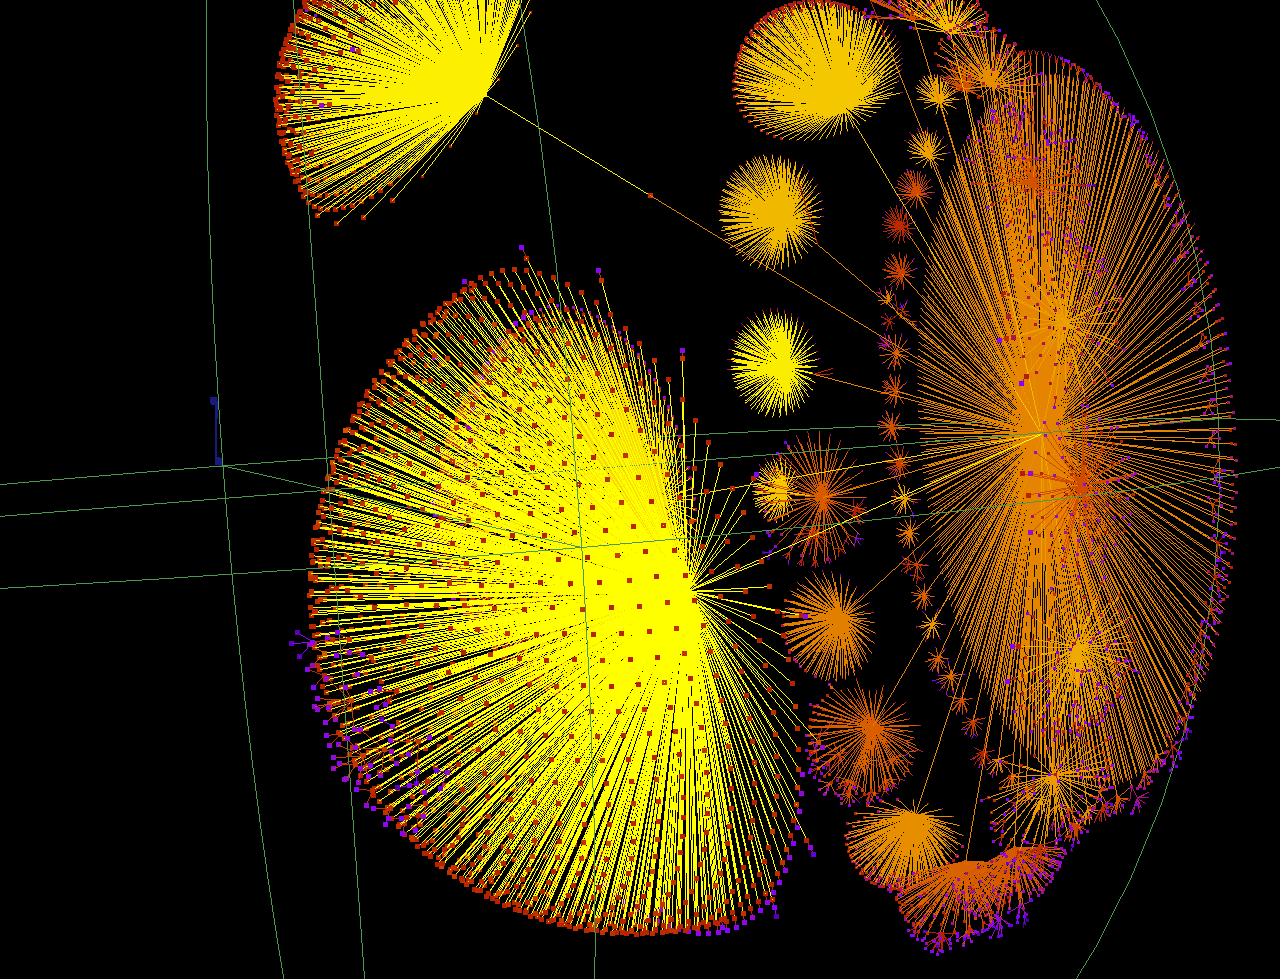
\includegraphics[width=\textwidth]{Closeness_walrus.png}
	\caption{Najstarszy graf, wizualizacja algorytmu closeness}
\end{figure}
\FloatBarrier\FloatBarrier
\FloatBarrier\FloatBarrier
\begin{figure}[h]
	\centering
	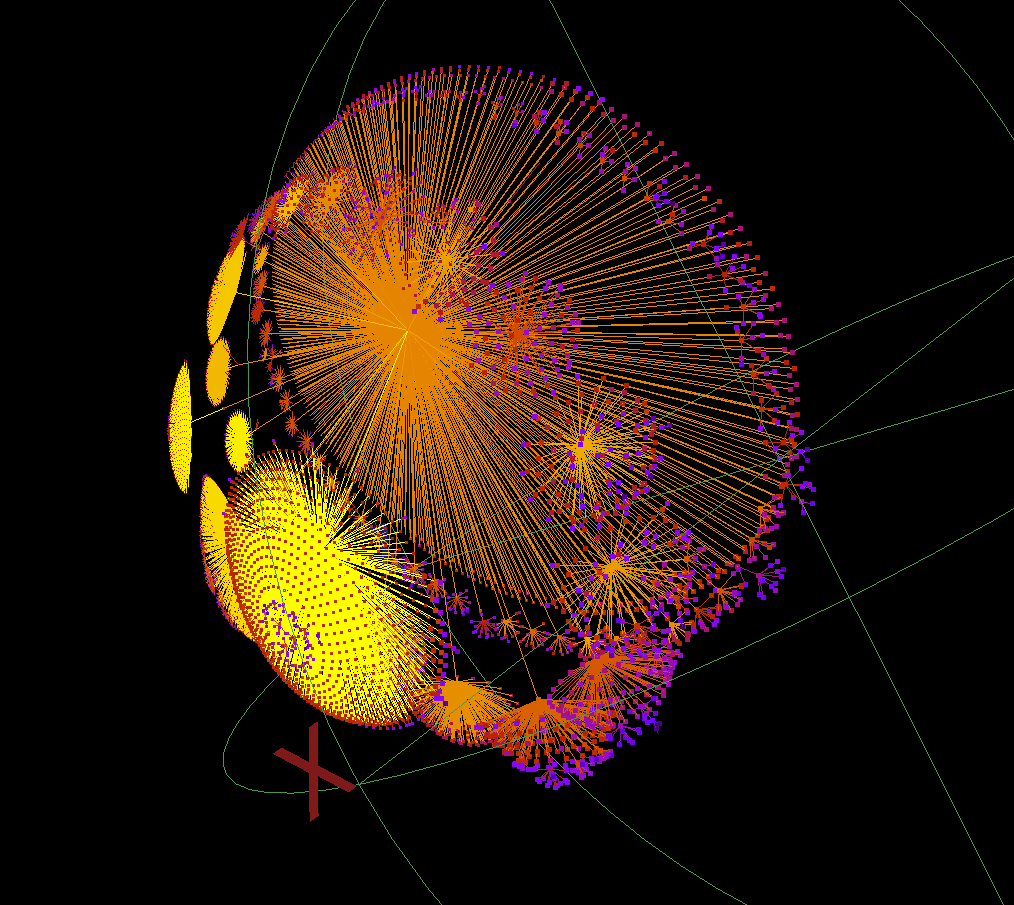
\includegraphics[width=\textwidth]{Closeness2_walrus.png}
	\caption{Najstarszy graf, wizualizacja algorytmu closeness - ujęcie 2}
\end{figure}
\FloatBarrier\FloatBarrier        
\FloatBarrier\FloatBarrier
\begin{figure}[h]
	\centering
	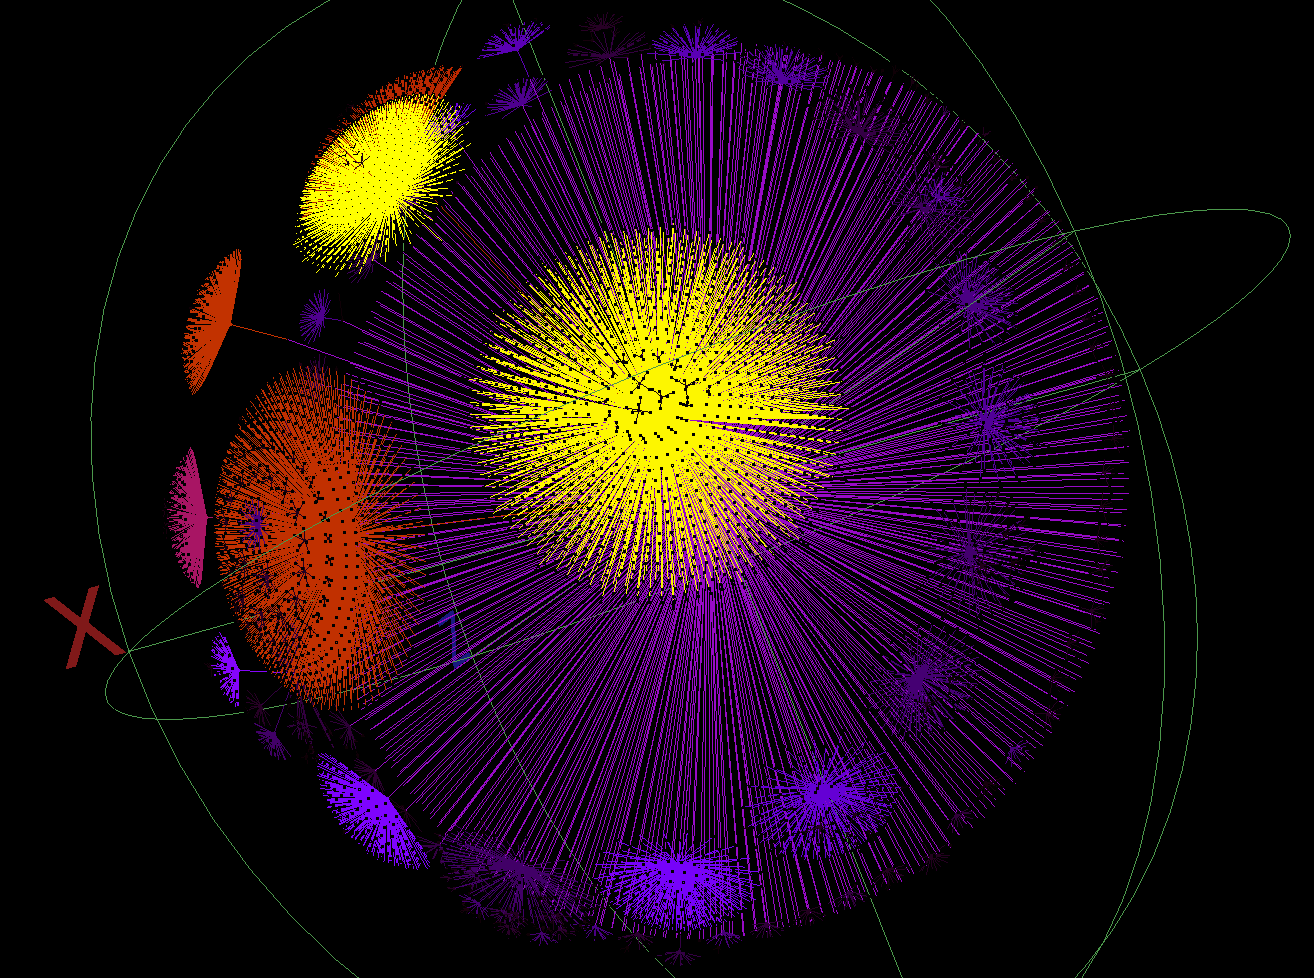
\includegraphics[width=\textwidth]{Pagerank_walrus.png}
	\caption{Najstarszy graf, wizualizacja algorytmu pagerank}
\end{figure}
\FloatBarrier\FloatBarrier
\FloatBarrier\FloatBarrier
\begin{figure}[h]
	\centering
	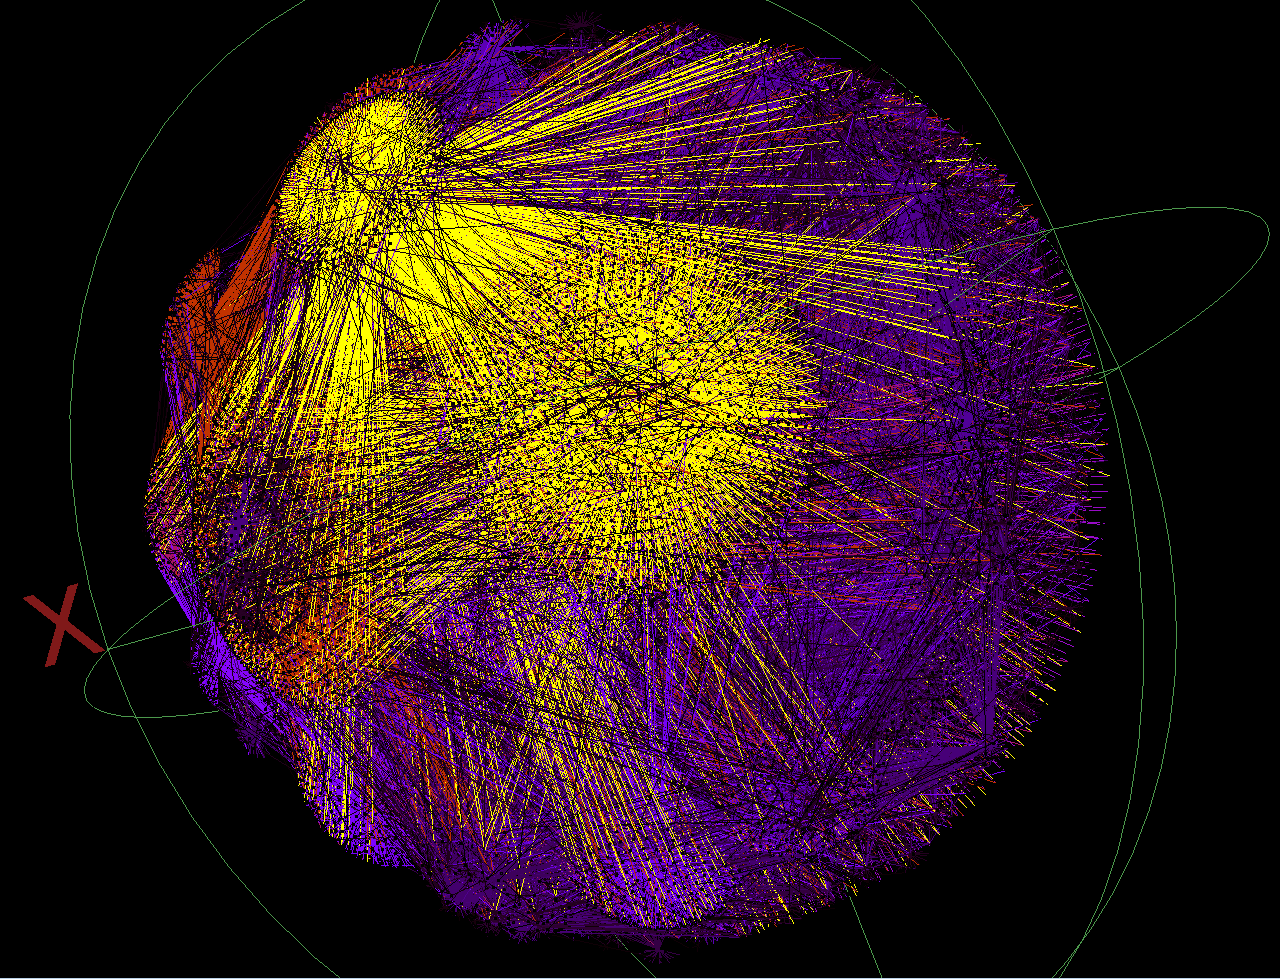
\includegraphics[width=\textwidth]{Pagerank2_walrus.png}
	\caption{Najstarszy graf, wizualizacja algorytmu pagerank - cały graf}
\end{figure}
\FloatBarrier\FloatBarrier    

Na powyższej ilustracji doskonale widać ogrom badanego grafu. Tak duża liczba krawędzi powoduje, że z wizualizacji ciężko cokolwiek wyczytać. Stąd rezygnacja z części z nich w pozostałych obrazach.
\chapter{Podsumowanie}
Badana sieć na przestrzeni kilku lat rozwijała się głównie poprzez dodawanie nowych węzłów na obrzeżach istniejącej już struktury. Rdzeń sieci, a zarazem jego najstarsza część, pozostał w dużej mierze niezmienny. W całym okresie charakterystyka sieci, badana algorytmami betweenness, closeness i pagerank zmieniała się. Dość ciekawą miarą jest w tym wypadku betweenness, gdyż pokazuje gdzie teoretycznie może wystąpić przeciążenie sieci. Taka miara pozwala na podjęcie decyzji o reorganizacji sieci tak, by zmniejszyć betweenness w danym węźle, albo umieścić tam odpowiednią infrastrukturę, która będzie sobie w stanie poradzić z takim obciążeniem. Niemałym problemem okazało się w projekcie odrzucenie zrzutów sieci, które odbiegały znacząco od pozostałych pod względem ilości wierzchołków. Takie dane niewątpliwie mogłyby znacznie zaburzyć wyniki wszystkich badanych miar, stąd należało je odrzucić uznając za błąd gruby. 

%\bibliographystyle{plalpha}
\bibliographystyle{plabbrv}

%UWAGA: bibliotekę referencji należy przygotować samemu. Dobrym do tego narzędziem jest JabRef.
%       Nazwę przygotowanej biblioteki wpisuje się poniżej bez rozszerzenia 
%       (w tym przypadku jest to "dokumentacja.bib")
\bibliography{bibliography}
%\appendix
%\include{dodatekA}
%\include{dodatekB}

%\chapterstyle{noNumbered}
%\phantomsection % sets an anchor
%\addcontentsline{toc}{chapter}{Indeks rzeczowy}
%\printindex

\end{document}
